% ******************************* PhD Thesis Template **************************
% Please have a look at the README.md file for info on how to use the template

\documentclass[custombib,a4paper,12pt,times,print,index,chapter]{Classes/PhDThesisPSnPDF}
\usepackage{graphicx}

% ******************************************************************************
% ******************************* Class Options ********************************
% *********************** See README for more details **************************
% ******************************************************************************

% `a4paper'(The University of Cambridge PhD thesis guidelines recommends a page
% size a4 - default option) or `a5paper': A5 Paper size is also allowed as per
% the Cambridge University Engineering Deparment guidelines for PhD thesis
%
% `11pt' or `12pt'(default): Font Size 10pt is NOT recommended by the University
% guidelines
%
% `oneside' or `twoside'(default): Printing double side (twoside) or single
% side.
%
% `print': Use `print' for print version with appropriate margins and page
% layout. Leaving the options field blank will activate Online version.
%
% `index': For index at the end of the thesis
%
% `draftclassic': For draft mode without loading any images (same as draft in book)
%
% `draft': Special draft mode with line numbers, images, and water mark with
% timestamp and custom text. Position of the text can also be modified.
%
% `abstract': To generate only the title page and abstract page with
% dissertation title and name, to submit to the Student Registry
%
% `chapter`: This option enables only the specified chapter and it's references
%  Useful for review and corrections.
%
% ************************* Custom Page Margins ********************************
%
% `custommargin`: Use `custommargin' in options to activate custom page margins,
% which can be defined in the preamble.tex. Custom margin will override
% print/online margin setup.
%
% *********************** Choosing the Fonts in Class Options ******************
%
% `times' : Times font with math support. (The Cambridge University guidelines
% recommend using times)
%
% `fourier': Utopia Font with Fourier Math font (Font has to be installed)
%            It's a free font.
%
% `customfont': Use `customfont' option in the document class and load the
% package in the preamble.tex
%
% default or leave empty: `Latin Modern' font will be loaded.
%
% ********************** Choosing the Bibliography style ***********************
%
% `authoryear': For author-year citation eg., Krishna (2013)
%
% `numbered': (Default Option) For numbered and sorted citation e.g., [1,5,2]
%
% `custombib': Define your own bibliography style in the `preamble.tex' file.
%              `\RequirePackage[square, sort, numbers, authoryear]{natbib}'.
%              This can be also used to load biblatex instead of natbib
%              (See Preamble)
%
% **************************** Choosing the Page Style *************************
%
% `default (leave empty)': For Page Numbers in Header (Left Even, Right Odd) and
% Chapter Name in Header (Right Even) and Section Name (Left Odd). Blank Footer.
%
% `PageStyleI': Chapter Name next & Page Number on Even Side (Left Even).
% Section Name & Page Number in Header on Odd Side (Right Odd). Footer is empty.
%
% `PageStyleII': Chapter Name on Even Side (Left Even) in Header. Section Number
% and Section Name in Header on Odd Side (Right Odd). Page numbering in footer

% Uncomment to change page style
%\pagestyle{PageStyleII}

% ********************************** Preamble **********************************
% Preamble: Contains packages and user-defined commands and settings
% ******************************************************************************
% ****************************** Custom Margin *********************************
% Add `custommargin' in the document class options to use this section
% Set {innerside margin / outerside margin / topmargin / bottom margin}  and
% other page dimensions
\ifsetCustomMargin
  \RequirePackage[left=37mm,right=30mm,top=35mm,bottom=30mm]{geometry}
  \setFancyHdr % To apply fancy header after geometry package is loaded
\fi
% Add spaces between paragraphs
%\setlength{\parskip}{0.5em}
% Ragged bottom avoids extra whitespaces between paragraphs
\raggedbottom
% To remove the excess top spacing for enumeration, list and description
%\usepackage{enumitem}
%\setlist[enumerate,itemize,description]{topsep=0em}

% *****************************************************************************
% ******************* Fonts (like different typewriter fonts etc.)*************

% Add `customfont' in the document class option to use this section
\usepackage{doi}

\ifsetCustomFont
  % Set your custom font here and use `customfont' in options. Leave empty to
  % load computer modern font (default LaTeX font).
  %\RequirePackage{helvet}

  % For use with XeLaTeX
  %  \setmainfont[
  %    Path              = ./libertine/opentype/,
  %    Extension         = .otf,
  %    UprightFont = LinLibertine_R,
  %    BoldFont = LinLibertine_RZ, % Linux Libertine O Regular Semibold
  %    ItalicFont = LinLibertine_RI,
  %    BoldItalicFont = LinLibertine_RZI, % Linux Libertine O Regular Semibold Italic
  %  ]
  %  {libertine}
  %  % load font from system font
  %  \newfontfamily\libertinesystemfont{Linux Libertine O}
\fi

% *****************************************************************************
% **************************** Custom Packages ********************************

% ************************* Algorithms and Pseudocode **************************

%\usepackage{algpseudocode}


% ********************Captions and Hyperreferencing / URL **********************

% Captions: This makes captions of figures use a boldfaced small font.
%\RequirePackage[small,bf]{caption}

\RequirePackage[labelsep=space,tableposition=top]{caption}
\renewcommand{\figurename}{Fig.} %to support older versions of captions.sty


% *************************** Graphics and figures *****************************

%\usepackage{rotating}
%\usepackage{wrapfig}

% Uncomment the following two lines to force Latex to place the figure.
% Use [H] when including graphics. Note 'H' instead of 'h'
%\usepackage{float}
%\restylefloat{figure}

% Subcaption package is also available in the sty folder you can use that by
% uncommenting the following line
% This is for people stuck with older versions of texlive
%\usepackage{sty/caption/subcaption}
\usepackage{subcaption}

% ********************************** Tables ************************************
\usepackage{booktabs} % For professional looking tables
\usepackage{multirow}

%\usepackage{multicol}
%\usepackage{longtable}
%\usepackage{tabularx}


% *********************************** SI Units *********************************
\usepackage{siunitx} % use this package module for SI units

%****************************** Degree symbol
\usepackage{gensymb}
% ******************************* Line Spacing *********************************

% Choose linespacing as appropriate. Default is one-half line spacing as per the
% University guidelines

% \doublespacing
% \onehalfspacing
% \singlespacing


% ************************ Formatting / Footnote *******************************

% Don't break enumeration (etc.) across pages in an ugly manner (default 10000)
%\clubpenalty=500
%\widowpenalty=500

%\usepackage[perpage]{footmisc} %Range of footnote options


% *****************************************************************************
% *************************** Bibliography  and References ********************

%\usepackage{cleveref} %Referencing without need to explicitly state fig /table

% Add `custombib' in the document class option to use this section
\ifuseCustomBib
   \RequirePackage[sort, authoryear]{natbib} % CustomBib
   \setcitestyle{round}

% If you would like to use biblatex for your reference management, as opposed to the default `natbibpackage` pass the option `custombib` in the document class. Comment out the previous line to make sure you don't load the natbib package. Uncomment the following lines and specify the location of references.bib file

%\RequirePackage[backend=biber, style=authoryear, citestyle=authoryear, sorting=nty, natbib=true]{biblatex}
%\bibliography{References/references} %Location of references.bib only for biblatex

\fi

% changes the default name `Bibliography` -> `References'
\renewcommand{\bibname}{References}


% ******************************************************************************
% ************************* User Defined Commands ******************************
% ******************************************************************************

% *********** To change the name of Table of Contents / LOF and LOT ************

%\renewcommand{\contentsname}{My Table of Contents}
%\renewcommand{\listfigurename}{My List of Figures}
%\renewcommand{\listtablename}{My List of Tables}


% ********************** TOC depth and numbering depth *************************

\setcounter{secnumdepth}{2}
\setcounter{tocdepth}{2}


% ******************************* Nomenclature *********************************

% To change the name of the Nomenclature section, uncomment the following line

%\renewcommand{\nomname}{Symbols}


% ********************************* Appendix ***********************************

% The default value of both \appendixtocname and \appendixpagename is `Appendices'. These names can all be changed via:

%\renewcommand{\appendixtocname}{List of appendices}
%\renewcommand{\appendixname}{Appndx}

% *********************** Configure Draft Mode **********************************

% Uncomment to disable figures in `draft'
%\setkeys{Gin}{draft=true}  % set draft to false to enable figures in `draft'

% These options are active only during the draft mode
% Default text is "Draft"
%\SetDraftText{DRAFT}

% Default Watermark location is top. Location (top/bottom)
%\SetDraftWMPosition{bottom}

% Draft Version - default is v1.0
%\SetDraftVersion{v1.1}

% Draft Text grayscale value (should be between 0-black and 1-white)
% Default value is 0.75
%\SetDraftGrayScale{0.8}

% *********************** Turn on draft watermark **********************************

%\usepackage{draftwatermark}
%\SetWatermarkLightness{0.9}



% ******************************** Todo Notes **********************************
%% Uncomment the following lines to have todonotes.

%\ifsetDraft
%	\usepackage[colorinlistoftodos]{todonotes}
%	\newcommand{\mynote}[1]{\todo[author=kks32,size=\small,inline,color=green!40]{#1}}
%\else
%	\newcommand{\mynote}[1]{}
%	\newcommand{\listoftodos}{}
%\fi

% Example todo: \mynote{Hey! I have a note}

% ************************ Thesis Information & Meta-data **********************
% Thesis title and author information, refernce file for biblatex
% ************************ Thesis Information & Meta-data **********************
%% The title of the thesis
\title{The causes and implications of orangutan flange plasticity}
%\texorpdfstring is used for PDF metadata. Usage:
%\texorpdfstring{LaTeX_Version}{PDF Version (non-latex)} eg.,
%\texorpdfstring{$sigma$}{sigma}

%% Subtitle (Optional)
%%\subtitle{Subtitle}

%% The full name of the author
\author{Noah Atkin}

%% Department (eg. Department of Engineering, Maths, Physics)
\dept{Department of Archaeology}

%% University and Crest
\university{University of Cambridge}
% Crest minimum should be 30mm.
\crest{
\includegraphics[width=0.2\textwidth]{University_Crest}}
%% Use this crest, if you are using the college crest
%% Crest long miminum should be 65mm
%\crest{
\includegraphics[width=0.45\textwidth]{University_Crest_Long}}

%% College shield [optional] 
% Crest minimum should be 30mm.
\collegeshield{\includegraphics[width=0.2\textwidth]{Figs/CollegeShields/LucyCavendish.eps}}


%% Supervisor (optional)
%% for multiple supervisors, append each supervisor with the \newline command
\supervisor{Dr. Sylvain Lemoine}
%Prof. C.D. Supervisor}

%% Supervisor Role (optional) - Supervisor (default) or advisor
% \supervisorrole{\textbf{Supervisors: }}
%% if no title is desired:
% \supervisorrole{}

%% Supervisor line width: required to align supervisors
\supervisorlinewidth{0.35\textwidth}

%% Advisor (optional)
%% for multiple advisors, append each advisor with the \newline command
\advisor{Word count: 30,976}
%Dr. B. Advisor}
     
%% Advisor Role (optional) - Advisor (default) or leave empty
 \advisorrole{}
%% if no title is required
% \advisorrole{}

%% Advisor line width: required to align supervisors
\advisorlinewidth{0.35\textwidth}


%% You can redefine the submission text:
% Default as per the University guidelines:
% ``This dissertation is submitted for the degree of''
%\renewcommand{\submissiontext}{change the default text here if needed}

%% Full title of the Degree
\degreetitle{Master of Philosophy in Biological Anthropological Science}

%% College affiliation (optional)
\college{Lucy Cavendish College}

%% Submission date
% Default is set as {\monthname[\the\month]\space\the\year}
%\degreedate{September 2014} 

%% Meta information
\subject{LaTeX} \keywords{{LaTeX} {MPhil Thesis} {Engineering} {University of
Cambridge}}


% ***************************** Abstract Separate ******************************
% To printout only the titlepage and the abstract with the PhD title and the
% author name for submission to the Student Registry, use the `abstract' option in
% the document class.

\ifdefineAbstract
 \pagestyle{empty}
 \includeonly{Declaration/declaration, Abstract/abstract}
\fi

% ***************************** Chapter Mode ***********************************
% The chapter mode allows user to only print particular chapters with references
% Title, Contents, Frontmatter are disabled by default
% Useful option to review a particular chapter or to send it to supervisior.
% To use choose `chapter' option in the document class

\ifdefineChapter
 \includeonly{Chapter3/chapter3}
\fi

% ******************************** Front Matter ********************************
\begin{document}
\frontmatter

\maketitle

% ******************************* Thesis Dedidcation ********************************

\begin{dedication} 

I would like to dedicate this dissertation to my patient mother whose unending support allowed me to venture into Suaq Balimbing and discover my passion for the "people of the forest".

\end{dedication}
% ******************************* Thesis Declaration ***************************

\begin{declaration}

I hereby declare that except where specific reference is made to the work of 
others, the contents of this dissertation are original and have not been 
submitted in whole or in part for consideration for any other degree or 
qualification in this, or any other university. This dissertation is my own 
work and contains nothing which is the outcome of work done in collaboration 
with others, except as specified in the text and Acknowledgements. This 
dissertation contains fewer than 35,000 words including appendices, 
bibliography, footnotes, tables and equations and has fewer than 150 figures.

% Author and date will be inserted automatically from thesis.tex \author \degreedate

\end{declaration}
% ************************** Thesis Acknowledgements **************************

\begin{acknowledgements}      

Firstly, I would first like to thank my supervisor, Dr. Sylvain Lemoine, for his assistance throughout the year, particularly for reviewing rough drafts of chapters, providing feedback, and his encouragement to share the results of my second chapter at the 2023 PSGB Spring Conference. I am deeply grateful for the interest in my professional development, his confidence in my ability to complete this research, and for accepting supervision of my project in the first place.

Secondly, I would like to thank Dr. Maria van Noordwijk at the University of Zürich for all her assistance. Primarily for providing access to the long-term data sets of the Tuanan Field Station, without which this project would not have been possible. I am particularly grateful for her feedback on Chapter 2, her encouragement to investigate this topic in the first place and suggesting lines of enquiry.

Thirdly, I would like to thank Dr. Caroline Schuppli and the Suaq Project for providing access to their long-term data set, without which cross-site comparisons would not have been possible. Additionally, I would like to thank her for taking a chance on me to work in Suaq Balimbing as a research assistant and starting me on the academic adventure I find myself in.

I would like to thank Dr. Julia Kunz, for providing early access to her manuscript reviewing the alternate mating strategies of male morphs and for providing her data set of female association with males at Suaq and Tuanan which greatly aided the production of Chapters 3 and 4. 

I would also like to thank my close friend Cameron Pearson for proofreading the entire dissertation before submission while on a delayed train to Manchester.

I gratefully acknowledge the Indonesian State Ministry for Research, Technology and Higher Education (RISTEKDIKTI), the Indonesian Institute of Science (LIPI), the Directorate General of Natural Resources and Ecosystem Conservation–Ministry of Environment \& Forestry of Indonesia (KSDAE-KLHK), the Ministry of Internal affairs, the Nature Conservation Agency of Central Kalimantan (BKSDA), the local governments in Central Kalimantan, the Kapuas Protection Forest Management Unit (KPHL), the Bornean Orangutan Survival Foundation (BOSF), and MAWAS in Palangkaraya as well as the Sumatran orangutan conservation Program (SOCP) and Taman Nasional Gunung Leuser (TNGL) in Medan for their permission and support to conduct this research. I'd also like to thank the Fakultas Biologi Universitas Nasional (UNAS) in Jakarta for their collaboration and support for the Tuanan and Suaq project and in particular Dr. Tatang Mitra Setia. 
 
Thank you to all researchers, students, volunteers, and local field assistants involved in the collection of the standard behavioural data for the long-term databases of Suaq Balimbing and Tuanan. I am also grateful to the local staff at the field sites and the associated offices. 

Finally, thank you to my partner Jessica Smith, for all of her love and support while I spent months measuring orangutan flanges, and for believing in me when I didn't.



\end{acknowledgements}

% ************************** Thesis Abstract *****************************
% Use `abstract' as an option in the document class to print only the titlepage and the abstract.
\begin{abstract}
Flanged male orangutans exhibit secondary sexual characteristics absent from their unflanged counterparts, the most prominent being their distinctive cheek pads or flanges. Since 1976, there have been observations of flanged males in poor body condition with flanges that appeared shriveled or deformed, a phenomenon tentatively referred to as "past-prime" in the literature. Various hypotheses have been proposed to explain this condition, from age-related degeneration to severe negative energy balances causing ketosis of the fatty content of the flanges. However, so far no attempts have been made to quantify changes in the shape of the flange over time or to prove the causes and social implications of such a condition. In this study, I analysed the relative size and area of the flange of two long-term orangutan field sites using existing photographic data sets and explored the correlations between decreased flange size and social behaviour. The key findings are as follows: 

1) Composite relative fluctuating asymmetry scores were higher in the Bornean field site compared to the Sumatran field site, which I suggest may be due to the lower overall fruit availability and comparatively poor ecological health of the Bornean field site. 

2) Flange measurements showed poor repeatability between photos taken on different days, which I suggest may be in part due to significant flange plasticity over time after their development. 

3) I found that flange width deterioration appears to be driven primarily by age and that individuals with diminished flanges produce more long calls per day. This suggests that the variance in the size of the flange after development is likely not due to ketosis, but may be driven by age-related deterioration of the muscle fibres and connective tissue that supports the structure of the flange. 

4) Older flanged males show significant changes in their long call behaviour, producing shorter long calls with fewer pulses. I suggest that these changes may due to need for recently flanged males to react strongly to local events to establish their presence, and also may hint at the energetic costs of producing long calls becoming more burdensome as individuals grow older. 
\end{abstract}


% *********************** Adding TOC and List of Figures ***********************

\tableofcontents

\listoffigures

\listoftables

% \printnomenclature[space] space can be set as 2em between symbol and description
%\printnomenclature[3em]

\printnomenclature

% ******************************** Main Matter *********************************
\mainmatter

%!TEX root = ../thesis.tex
%*******************************************************************************
%*********************************** First Chapter *****************************
%*******************************************************************************
\ifpdf
    \graphicspath{{Chapter1/Figs/Raster/}{Chapter1/Figs/PDF/}{Chapter1/Figs/}}
\else
    \graphicspath{{Chapter1/Figs/Vector/}{Chapter1/Figs/}}
\fi
\chapter{Introduction}  %Title of the First Chapter

Orangutans are unique among primates in that they are bimature and males show two distinct male morphs: the initial "unflanged" morph and the subsequent "flanged" morph \citep{Knott.2008}. Flanged males possess many secondary sexual characteristics that the unflanged male lacks, including a saggitial crest, a throat sac capable of making long calls, and fat cheek pads, also known as flanges \citep{Galdikas.1978cv}.

Although the development of these morphs in an individual is sequential, the unflanged form is not a "subadult" form, as they are sexually active and can cooperatively breed with females (though forced mating is more common) \citep{Knott.2009, Kunz.2023}. The transition between the two morphs can be arrested for many years, and in some habitats this transition can be arrested for decades \citep{Dunkel.2013}. 

Only recently have the mechanisms that trigger the development of the flange begun to be understood, which appears to be a mixture of social and endocrinological factors, including proximity to other flanged males and the presence of a stable local dominance hierarchy \citep{Dunkel.2013xnm, Marty.2015, Prasetyo.2019}.

Given that the transition from unflanged male to flanged male is irreversible, there remains debate about the plasticity of these traits after development, or whether their morphology is "fixed" during development. While throat sacs and associated long calls have been extensively studied in recent years, less attention has been paid to flanges and their plasticity after initial development \citep{Spillmann.2016}.

Physiologically, flanges are bilateral fleshy disc-shaped structures composed of fibrous connective tissue, adipose tissue, and muscle fibres \citep{Straus.1942,Winkler.1989}. These conspicuous features are believed to play a role in female mate choice, and are often used as part of individual identification \citep{Utami.2002km8, Kappeler.2004}

Various reports have been made from different field sites suggesting significant plasticity of the flange after development; however, the suggested causes or impacts of such a change have not yet been thoroughly investigated \citep{Galdikas.1978cv,Galdikas.1985, Knott.2009}.


The objectives of this dissertation are to:
\begin{enumerate}
    \item Quantify relative flange size using historic photographic data sets
    \item Examine how three key factors: age, fruit availability, and antagonistic male-male social interactions, shape the morphology of orangutan flanges after their development
    \item Examine shifts in behaviour from these individuals to estimate impacts or social correlates of reduced flange size
    \item Delve deeper into the cause(s) using long term behavioural data sets to gain wider insight into how this factor(s) shape flanged male behaviour
\end{enumerate}

By analysing two different populations in different species and ecologies, I hope to examine the role that social and nutritional factors play in the plasticity of these secondary sexual characteristics and provide greater insight into how these conspicuous traits impact, and are impacted, by their social and ecological environment.

\section{Structure of the dissertation}
This dissertation is split into 5 chapters. The first chapter is a general introduction to orangutans, their sexual dimorphism and bimaturism, and a short review of the limited articles that have observed this condition. 

The next three chapters are written as manuscripts for scientific papers. However, some of the methodology and data sets overlap between chapters, for example the facial landmarks measured in Chapter 2 form the basis of flange measurements from Chapter 3. 

In Chapter 2, I examine differences in fluctuating asymmetry in facial landmarks between sites using previously collected photographic data sets. I predicted that fluctuating asymmetry would be higher in the Bornean field site, and hypothesised that it was due to the differences in fruit availability in each site, the differential impacts of fire and historical human disturbance between sites.

In Chapter 3, I investigated the claim that the flange size varies over the lifetime of a flanged male. I predicted that due to the adipose content of the flanges, the reduction in the flange size would follow periods of low fruit availability. Additionally, I predicted that the psychoendocrinilogical factors that have been previously hypothesised to inhibit initial flange development would play a similar role after flange development; however, I predicted that this effect would be to a lesser extent than fruit availability. 

In Chapter 4, I investigate the impact of age on flanged male mating success and long call behaviour, including female association duration. I predicted a slow decrease in female association over time, in line with other primates; and that the energetic costs of long calls would be felt more strongly by older individuals leading to a change in their composition, frequency, or duration.

Finally, I conclude with Chapter 5, which summarises and synthesises the results from the main research chapters. 
\begin{figure}[htbp!] 
\centering    
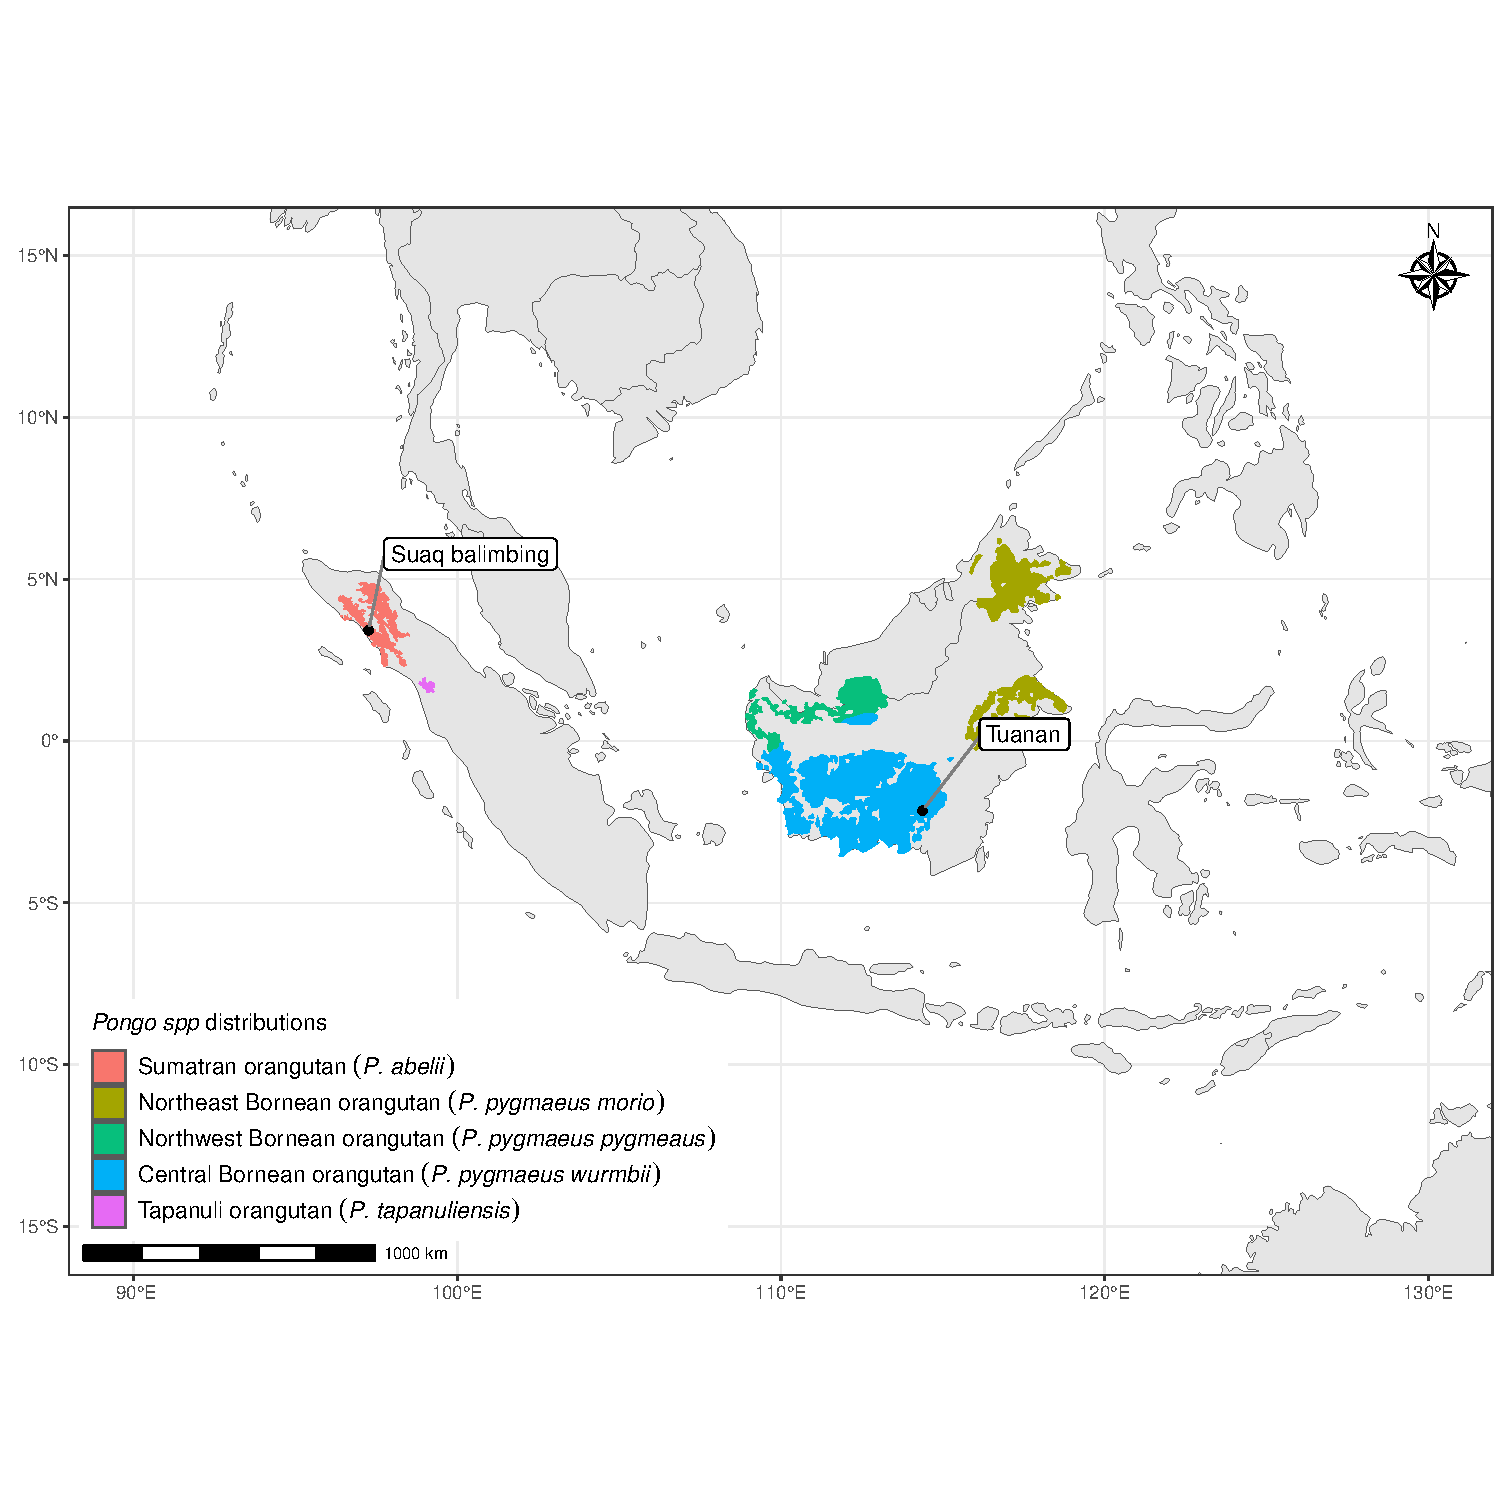
\includegraphics[width=1.0\textwidth]{mawasplot.eps}
\caption{Map illustrating orangutan distribution in Sumatra and Borneo. Locations of the field sites associated with the data in this dissertation are highlighted.}
\label{fig:A map of the distribution of wild Pongo spp. populations across Sumatra and Borneo, with the positions of Suaq Balimbing and Tuanan shown.}
\end{figure}


%********************************** %First Section  **************************************
\section{Introduction}
\subsection{Taxonomy \& distribution}
 %Section - 1.1 

Orangutans are the only extant members of the Ponginae sub-family, which split from the Homininae branch roughly 14 million years ago \citep{Grabowski.2017}. Their genus \textit{Pongo} originated 6 to 5 million years ago, and while historically members of the genus were found across mainland south-east Asia, since the late 1600s they are only located on the islands of Sumatra and Borneo \citep{Spehar.2018}.

The entire population was originally classified as a single species under the biological species concept, \textit{ Pongo pygmaeus}, despite the observed differences in morphology, behaviour, and ecology between Sumatran and Bornean populations. However, calls to have them classified as separate species grew in 1990s based on genetic evidence of species-level divergence between the two populations. Gel electrophoresis of isozymes and fibroblast proteins indicated indicated a split 1.5 million years ago between the Sumatran and Bornean populations, and mitochondrial DNA differences suggested a relatedness between the two species similar to that between horses and donkeys \citep{Janczewski.1990,Xu.1996}. These calls were officially recognised in 1999, when the Orangutan Action Plan officially recognised the Bornean orangutan (\textit{Pongo pygmaeus}) and the Sumatran orangutan (\textit{Pongo abelii}) as separate species \citep{Groves.1999}. 

This reclassification also recognised 3 subspecies of the Bornean orangutan based on their geographic position and multivariate analysis of their skull shapes and molars: 
\begin{itemize}
\item \textit{P. p. pygmaeus}, located in the north west of Borneo
\item \textit{P. p. wurmbii}, located in the south of Borneo
\item \textit{P. p. morio}, located in the north-east of Borneo in 2 separate patches
\end{itemize}

Finally, in 2017 the Tapanuli orangutan (\textit{Pongo tapanuliensis}), located only in the Batang toru ecosystem south of Lake Toba, was classified as a separate species based on its unique morphology, genetics and habitat; and is more closely related to the Bornean population than the Sumatran population only 400km north of them \citep{Nater.2017}. 
%********************************** %Second Section  *************************************

\section{Conservation status}
 %Section - 1.2

Great apes are particularly at risk to anthropogenic threats due to their nutritionally constrained dispersal ability, low population density, poor thermoregulation, and slow life history \citep{Carvalho.2019}. These factors are particularly noticeable in orangutans, for whom a 1\% population loss can drive a population to extinction \citep{Wich.2008}. Even under ideal conditions, an orangutan population can only grow in size by 2\% annually, and currently all orangutan populations are declining \citep{Utami-Atmoko.2016}.

All species of orangutan are currently classified as "Critically endangered" by the IUCN Red List and all have declining population trends. Current estimates of their population can be seen in Figure 1.2.

\begin{table}
    \centering
    \resizebox{\textwidth}{!}{%
\begin{tabular}{l c c c c r }
\hline 
\multirow{2}{*}{\textit{Pongo spp.}} & \multicolumn{4}{c}{Population Size}  & \multirow{2}{*}{References}\\ 
\cline{2-5}
  & Wild & Rehab.  & Zoo & Total (Estimated) \\ 
\hline
\textit{P. abelii} & 13,000 - 14,000 & Unk. & 319  & 13,319 - 14,319 &  \citep{Wich.2016, Utami-Atmoko.2016, na8}\\

\textit{P. pygmaeus morio} & 3,000 - 4,500 & Unk. & < 616  & 3,000 - 5,116 & \citep{Utami-Atmoko.2016, na8} \\\


\textit{P. pygmaeus pygmaeus} & 10,000 - 11,000 & Unk. & < 616 & 10,000 - 11,616 & \citep{Utami-Atmoko.2016, na8}\\

\textit{P. pygmaeus wurmbii} & 34,000 - 35,000 & Unk. & < 616 & 34,000 - 35,616 & \citep{Wich.2016, na8}\\

\textit{P. tapanuliensis} & < 800 & Unk. & Unk. & < 800 &\citep{Nater.2017, Laurance.2020, na8}\\
\hline 
\end{tabular}
}
\caption{Population estimates of orangutan species and sub-species. Zoo population estimates are based on the 2022 International Studbook of the Orangutan \citep{na8}.}
\end{table}

Orangutan spp. originated around 3 million years ago around the foothills of the Himalayas \citep{Rijksen.1999}. They are believed to have spread across the foothills of mountain ranges through South East Asia to the Sunda islands of Borneo, Sumatra, and Java \citep{Meijaard.2022}. As humans spread across this area, their population growth, slash and burn agriculture, hunting pressure, and environmental changes limited the range of orangutans to only two islands \citep{Rijksen.1999}. Today, the main threats to all species of orangutans are land use change, the illegal pet trade, and illegal hunting \citep{Rijksen.1999}. Palm oil plantations are a significant threat to surviving intact forest fragments and remain a major source of new land for plantations despite calls for industry reform. It is estimated that more than 50\% of Indonesian forest were lost to palm plantations between 1990 and 2005 \citep{Gibbs.2010}. Primary forests in carbon-rich peatlands are cleared to make room for palm oil plantations, which directly impacts the climate as well as biodiversity \citep{Gaveau.2009}. 40\% of palm oil in Indonesia and Borneo is produced by small landholders, whose disparate monocultures increasingly fragment existing orangutan populations, reducing the size of sub-populations to unviability \citep{Wich.2008v8i0d}. Of the estimated 100,000 orangutans that were killed between 1999 and 2015, most are estimated to have been killed due to selective logging in primary forests, as opposed to forest clearing or direct human-wildlife conflict \citep{Voigt.2018}. 

The Tapanuli orangutan faces a specific immediate threat due to the construction of a hydro-dam that is being constructed in the only intact forest patch currently connecting the three sub-populations \citep{Nater.2017,Laurance.2020}. The project, which is being implemented by Sinohydro as part of the Belt and Road Initiative, is highly politicised within Indonesia and many senior orangutan researchers who have been vocally critical of the project have been banned from conducting any further research in Indonesia \citep{Pramono.2022,CNN.2022}. Current projections estimate that construction will drive 2 of the sub-populations to unviability \citep{Wich.2019}. The third sub-population may remain viable, provided that planned logging concessions and gold mine expansion are not carried out, and all deforestation and orangutan killings stop permanently in the region \citep{Laurance.2020}. Defenders of the project propose the development of ecological corridors between the remaining sub-populations as a mitigation strategy, however, critics claim that there is currently a lack of evidence as to whether orangutans will use these corridors and question their effectiveness in linking the surviving sub-populations \citep{Kuswanda.2022}.

%********************************** % Third Section  *************************************
\section{Life history}  %Section - 1.3 

\label{section1.3}

Orangutans have the slowest life history of any great ape (except humans), with an inter-birth period of around 8 years \citep{Wich.2008t6}.  As arboreal primates with large home ranges and live forests characterised by a wide variation in food availability, acquiring ecological competence quickly is essential \citep{Noordwijk.2018}. Juveniles spend all of their time within 100m their mother until the age of 6-8 years, from whom they learn the majority of their skills through peering behaviour \citep{Wich.2008t6}. Following lactation, the ability of the female to conceive again is driven by the high availability of fruits so that they can reach the necessary physical condition \citep{Spillmann.2016}. Mothers adjust their own diet based on the ecological competence of their child and their ability to process specific foods, allowing the offspring to maximise opportunities for learning \citep{Mikeliban.2021}. Orangutans are mainly frugivorous, and fruits comprise the majority of their diet when available \citep{Galdikas.1988}. However, they are opportunistic feeders and also eat leaves, bark, pith, insects, small vines, and honey \citep{Galdikas.1988}. On rare occasions, males have been observed eating slow lorises in both Sumatra and Borneo \citep{Hardus.2012, Makur.2022}.

In addition to acquiring food, offspring need to learn how to build nests that orangutans generally create daily \citep{Prasetyo.2008}. Individuals from different areas show cultural modifications in their nest building behaviour, including covers and "pillows" \citep{Russon.2007}. Orangutans have been shown to carry specific leaves for hours to use them as part of their nest for that evening \citep{Russon.2007}. Due to orangutan female philopatry, juveniles show sex-specific attention biases as they age. Females target the majority of their peering behaviour towards their mother, however male juveniles spend a larger proportion of time peering at other individuals \citep{Ehmann.20216zj}. This is suggested to be in preparation for later ranging behaviour after the males reach independence.  Between the ages of 8-12, adolescents spend their time within their mothers home range, but living independently \citep{Wich.2008v8i0d}. After this period, male orangutans disperse in search of a new home range \citep{Morrogh-Bernard.2011zwh}. It is still unknown how far male orangutans travel, or for how long, but this ranging behaviour allows male orangutans to act as cultural vectors, spreading behaviours across sub-populations \citep{Mörchen.202378o}. Females acquire a new home range adjacent to their mothers and remain there for the rest of their life \citep{Wich.2008v8i0d}.  Unlike other great apes, orangutans are semi-solitary (due to the fluctuations in food availability) and their level of day-to-day socialisation depends on their population density, life stage, sex, and environment \citep{Wich.2008t6}. 

\section{Bimaturism and orangutan male morphs}
\subsection{Bimaturism}
Male orangutans are bimature \textit{ie} there are two sexually active male morphs capable of siring children: the flanged male and the unflanged male \citep{Galdikas.1985}. This is unique among primates, even though some primate species show different male morphs, such as the mandrill, these changes are reversible, and the "immature" form is not a case of arrested development \citep{Setchell.2001}. Interestingly, in some sites the transition from unflanged to flanged can be arrested for decades and the proportion of flanged males to unflanged males varies according to the local ecology of the site \citep{Dunkel.2013xnm, Kunz.2023}. \citet{Pradhan.2012} suggests part of the reason why elongated development arrest is not seen in other species more commonly is that it requires a very low adult mortality rate to be an evolutionary stable strategy.  

The ultimate causes of the differences between individuals in the timing of bimaturism are due to the evolutionary costs and benefits of becoming a flanged male: Increases in intrasexual competition vs. increases in perceived attractiveness. In Sumatra, population densities of orangutans are generally higher due to decreased variability in fruit availability and higher overall fruit production. This, in turn, reduces average home range sizes as there is reduced need to range widely for food, increasing the potential for males to monopolise access to females. This results in more stable dominance hierarchies, which increases the relative cost for an unflanged male to become flanged. However, when dominance hierarchies are unstable, the best strategy is to maximise the number of copulations, and as flanged males can easily defeat unflanged males we find a higher proportion of flanged orangutans under these conditions.

Although the evolutionary strategy for bimaturism is well accepted, the proximate triggers for bimaturism are not fully understood. The nutritional state does not appear to play a role in the initiation of the transition, as individuals with negative energy balance can still undergo the change \citep{Prasetyo.2021}. A hypothesis for how the transition is arrested is due to the psychoendoneuroligcal impact of social interactions that cause persistent stress in orangutans, suppress testosterone and increase cortisol levels \citep{Kingsley.1982}. \citet{Thompson.2012} found that testosterone levels in captive flanged males that had undergone developmental arrest were significantly lower than in males who had not, which may be an indication that early life testosterone levels predict the timing of bimaturism, but could also be due to an increase in testosterone levels after this transition. These results were reinforced by studies on wild orangutan males that showed a significant increase in testosterone metabolites in faecal samples in flanged males compared to unflanged males \citep{Marty.2015rzq}. However, this study did not find a significant difference in cortisol metabolite levels between the two morphs, which would be expected under the hypothesis. \citet{Marty.2015} suggests these results may be due to a stress avoidance strategy on the part of unflanged males to avoid conflict and that flanged males experience greater levels of competition, increasing their cortisol levels. \citet{Prasetyo.2021} found in a study of captive male orangutans that flanged males actually had the highest cortisol levels, compared to unflanged and developing males, but these results may have been in large part due to the solitary captive housing of flanged males in the study and the difference in energy intake. Ultimately, the proximate causes triggering bimaturism remain unknown and due to the differences in hormonal profiles between captive and wild orangutans, a large-scale assay of hormonal metabolites on a wild population where social behaviour is well studied may be required to unpack the relationships between these factors.

\subsection{Unflanged males}
Unflanged males vary in size, with young adults having a body mass similar to females, while fully grown unflanged males have a body mass between females and flanged males \citep{Kralick.2021}. Although they lack the fully developed secondary sexual characteristics of the flanged male, unflanged males have fully developed testes and have successfully sired offspring in captivity and in the wild \citep{Utami.2002km8}.  Due to the lack of ability to make a long call, unflanged males use a "silent searching" mating strategy \citep{Knott.2008}. Compared to flanged males, they range significantly more to increase the chance of locating females, and occasionally travel together without antagonistic interactions \citep{Setia.2008}.  Due to the preference of females for flanged males, unflanged males often resort to forced copulation, a rarity among great apes \citep{Knott.2009y9d}. Females can employ mating strategies to negate the worst of these problems by staying in the vicinity of flanged males and approaching long calls to shake off persistent unflanged males \citep{Knott.2009}. Unflanged males generally move away from long calls upon hearing them, despite flanged males being generally tolerant to unflanged males in their vicinity \citep{Spillmann.2010}. 

\subsection{Flanged males}
Flanged males are approximately twice the size of females and possess several secondary sexual characteristics that the unflanged male lacks \citep{Prasetyo.2021}. Flanged males have more body hair, a sagittal crest, and distinctive cheek pads, known as flanges \citep{Galdikas.1978}. Flanged males use a "wait and call" mating strategy, attracting females to their location by producing long calls, distinctive vocalisations that travel up to 1km \citep{Knott.2008, Utami.2002km8, Prasetyo.2019}. Newly immigrated flanged males employ a "challenge calling" strategy, by calling much more frequently than existing males in order to establish their presence in an area \citep{Hayward.2018}. 

The flanges, which are bilateral discs on each side of the face, are the most conspicuous secondary sexual characteristic that male orangutans develop, which are primarily formed of fat deposits bound to fibro-fatty tissues \citep{Straus.1942}. Any additional function of the flange beyond an indicator of fitness is somewhat unknown; however, most hypotheses link the function of the flange to the long call. \citet{Galdikas.1983} suggested that the slightly concave shape of the flange allows the individual to better locate the source of other long calls, while \citet{Mitani.1985ak1m} suggested that the shape allows individuals to focus their call in a specific direction. Despite these hypotheses, the acoustic impact of the flange has not yet been methodologically tested.

Interactions between flanged males are rare despite their overlap in home ranges and density within the forest, which is likely due to the long calls acting as a spacing mechanism \citep{Spillmann.2016}. When flanged males do meet, their interactions are almost always aggressive, and although lethal violence is uncommon, these antagonistic interactions commonly result in injuries, including as severe as the removal of digits \citep{Setia.2008}.  

\subsection{The "past-prime" flanged male}
The term "past-prime" was first used to describe a flanged male in 1978, where \citet{Galdikas.1978} described a focal individual, named PP, at the Tanjung Puting Reserve as "past his prime". They noted that PP spent significantly less time ranging compared to other flanged males in the area, and habituated to the human observers relatively quickly compared to the other flanged males in the field site. PP was described as different from the other flanged males based on their "\textit{sunken wrinkles and diminished cheekpads}", and PP died one year after habituation. Galdikas described another male with a flange that had been found in the same condition a few years later \citep{Galdikas.1978}. The individual had died approximately 12 hours before observation based on the level of decomposition; however, due to their condition no behavioural changes were observed. 

Since then it has been reported at multiple field sites that some orangutans have flanges that are shrivelled or deflated in appearance, however there is some disagreement on the ultimate cause of the condition \citep{Knott.2009, Dunkel.2013}.  \citet{Knott.2009} also suggests that the primary cause is age, but hints at loss of dominance being also a causative factor. Changes in secondary sexual characteristics associated with loss of dominance are observed in other primates, as mandrills that have lost alpha status show a reduction in the extent of red sexual skin colouration \citep{Setchell.2001}. Knott stated that the "past-prime" male "\textit{display[s] greatly diminished cheek flanges, they give significantly fewer long calls, have significantly lower testosterone levels and energy expenditure, mate infrequently, are less aggressive toward other males, and are subordinate to prime males}". However, while Knott began initial research in this area, no peer-reviewed articles have been published on the condition so far \citep{Knott.2009b}.  \citet{Dunkel.2013} however suggests poor body condition caused by reduced food availability as a possible cause of the condition, citing the seasonal variation in fruit production experienced at a number of field sites. 

Despite these observations, no peer-reviewed paper has examined the causes or social implications of the condition. Additionally, whether this is a threshold condition or is instead reflective of general level of flange plasticity after their initial development, which may be reflective of multiple causative factors, is also unknown.\label{Chapter1}
%!TEX root = ../thesis.tex
%*******************************************************************************
%****************************** Second Chapter *********************************
%*******************************************************************************
\ifpdf
    \graphicspath{{Chapter2/Figs/Raster/}{Chapter2/Figs/PDF/}{Chapter2/Figs/}}
\else
    \graphicspath{{Chapter2/Figs/Vector/}{Chapter2/Figs/}}
\fi
\chapter{Measuring fluctuating asymmetry from long term field sites: A case study on \textit{Pongo} spp.}

Fluctuating asymmetry is a random non-directional deviation in symmetry on bilateral features caused by developmental instability. Previous studies have indicated that elevated levels of fluctuating asymmetry are correlated with negative health outcomes and reduced perceived attractiveness. It has been suggested that secondary sexual traits may be more sensitive to fluctuating asymmetry due to their high metabolic cost and subsequent use as an unbiased indicator of fitness. In this study, I use historic long term photographic data sets from two field sites to examine the variance in facial fluctuating asymmetry in flanged males across two sub-populations, and examine whether fluctuating asymmetry in flanges can be observed. Composite relative fluctuating asymmetry scores were higher in the Bornean field site compared to the Sumatran field site, which I suggest may be due to the lower overall fruit availability and comparatively poor ecological health of the Bornean field site. Flange measurements showed poor repeatability between photos taken on different days, which I suggest may be in part due to significant flange plasticity over time after their development. This study indicates the usefulness of historic photographic data sets for examining changing ecological conditions and their implications on wild animal health.
 \pagebreak

\section{Introduction}
Biologists differentiate between 3 types of asymmetry: Directional asymmetry, antisymmetry, and fluctuating asymmetry (FA) (Fig. \ref{fig:examplefaplots}). Directional asymmetry (DA) is where a trait value is larger on one side of the body compared to the other across a population, for example, in humans the right gonad tends to be larger than the left \citep{MITTWOCH.1975}. In contrast, antisymmetry (AS) is where the trait value is asymmetric, but there is no preference of which side is larger across a population \textit{i.e.} it can be larger on either side of the body \citep{Zakharov.20223bp}. For example, largemouth bass show AS in their limb usage and turning direction which is maintained through negative frequency-dependent natural selection as their prey (freshwater gobies) are also antisymmetric \citep{Yasugi.2012}. While both DS and AS can have fitness benefits in specific organisms and result from normal development, fluctuating asymmetry (FA) is an indicator of developmental instability \citep{Valen.1962}.


\begin{figure}[h]
    \centering
    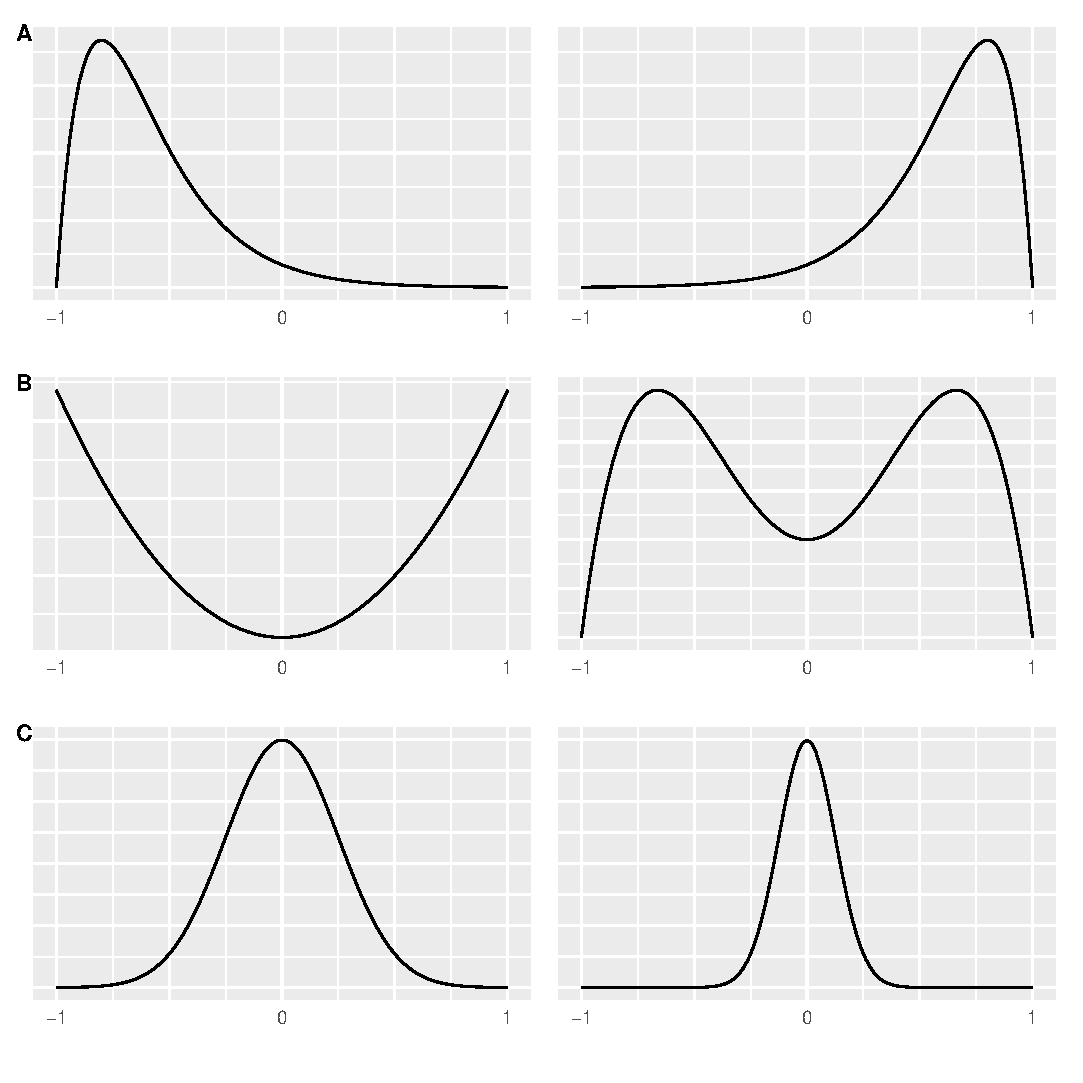
\includegraphics[width=0.75\textwidth]{Chapter2/Figs/Vector/spee.eps}
    \caption{Example population trait values under different types of asymmetry. 
A. Directional asymmetry. 
B. Antisymmetry. 
C. Fluctuating asymmetry. }
    \label{fig:examplefaplots}
\end{figure}

\pagebreak
Fluctuating asymmetry (FA) is minor non-directional deviance in trait values from perfect bilateral symmetry and is caused by environmental or genetic developmental instability (DI) \citep{Palmer.1986}. The presence of FA across organisms has been shown in laboratory conditions and in the wild across organisms and stressors. These stressors can be environmental (e.g., low food availability, pollution, social stress) or genetic (e.g., hybridisation, genetic disorders, inbreeding) \citep{Beasley.2013, Leung.1996, VØLLESTAD.1999}. In insects, meta-analyses have shown that FA is a sensitive biomarker to environmental stress across a variety of different traits, and is caused by a variety of stressors. However, the sensitivity of a particular trait to a specific stessor varied between different traits \citep{Beasley.2013}. Given the cost of maintaining homeostatic development, buffering against FA is likely to be prioritised in traits vital for survival \textit{e.g.} symmetry in leg length is important for efficient locomotion. Therefore, traits of relatively low functional importance are likely to experience more FA compared to vital ones, even under low external stress \citep{Leung.1997}. Together, these meta-analyses highlight the importance of trait selection when measuring FA, with attention paid to the particular ecology and functional role of each trait \citep{Landi.2021}.

At the population level, higher FA scores are more common in populations undergoing stress, meaning that FA could be used as a tool to monitor anthropogenic impacts on animals. Several studies have supported this assertion. In mammals, \citet{Kucheravy.2022} has shown an increase in FA of whisker spots in polar bears since 2003, which correlates with significant habitat degradation due to climate change. In birds, wing and tarsus FA was found to be significantly higher in forest fragments compared to continuous forest in 100 different species in the Brazilian south eastern Atlantic rainforest \citep{Anciães.2000}.  FA could also be used as a method of monitoring threatened populations, previous studies on Cuvier's gazelle have shown that increased levels of FA in horn length are strongly correlated with the coefficient of inbreeding, which in turn is strongly correlated with the proportion of abnormal sperm in the ejaculate \citep{Roldan.1998}. 

In addition to wild animals, FA is an important tool for monitoring captive or managed populations. Zoo animals are often endangered and managed populations generally have significantly lower genetic diversity compared to wild populations. Low genetic diversity has been associated with increased levels of FA in many organisms \citep{Leary.1989}. In healthy populations FA has very low heritability; however, it has been hypothesised that epistasis caused by low population genetic diversity, hybridisation between species, or rapid environmental change can cause additive genetic variation for FA, which in turn reduces the ability of populations to buffer against environmental change \citep{Leamy.2005}. As such, it has been suggested that populations with small effective population sizes are more sensitive to FA caused by environmental stress \citep{Knierim.2007}. This has been observed across gorilla subspecies, where facial asymmetry mirrors known genetic diversity, with significantly inbred mountain gorillas showing significantly higher facial FA compared to western lowland gorillas \citep{McGrath.20220bl}.

\subsection{Fluctuating asymmetry as a measure of health}
Multiple studies have linked increased fluctuating asymmetry in primates with negative health outcomes, however, this issue is controversial (see Section 2.1.2). 

In western lowland gorillas, canine FA correlated strongly with both the year of collection, due to increased human encroachment into their habitat, decreasing the availability of high-quality food resources \citep{Manning.1994}. In captive chimpanzees, facial FA was positively correlated with zookeeper reports of negative physical and mental health symptoms \citep{Sefcek.2007akp}.
Some of these relationships have also been seen in humans, \citet{Thornhill.2006} found that increased levels of body FA were correlated with self-reported health issues. Furthermore, increased levels of fluctuating asymmetry has also been linked to higher BMI in women, and the number of reported health conditions in both sexes \citep{Milne.2003, Al-Eisa.2004}. Notably however, there appears to be no link between FA and a number of common indicators of overall health in recent studies, including cardio-respiratory fitness, blood pressure, or blood cholesterol levels \citep{Milne.2003, Thornhill.2006, Dongen.2011}. This may be in part due to the minimisation of environmental stressors in modern western societies, which makes the underlying FA too small to measure. In contrast, bioarcheological studies on historic human cranial FA have indicated previous links between malnutrition and cranial FA in several different locations around the world \citep{DeLeon.2007,Dongen.2011,Jung.2016}.

\subsection{Issues with fluctuating asymmetry as a measure of health}
Whether FA can be universally used as a useful tool for monitoring population health has been questioned, for two notable reasons. 

Firstly, there is the inconsistency in studies regarding the relationship between FA and sexual selection, health, and individual condition. While meta-analyses have been published showing small but significant relationships between FA and population health and environmental stressors, individual studies are still mixed on the relationships between FA and population/individual outcomes.  This may be in part due to poor trait selection; as it has been hypothesised that sexually selected traits may undergo greater levels of FA compared to nonsexually selected traits, however, previous meta-analyses have not shown such a relationship. However, this inconsistency may also be due to the nature of FA itself, as the variance in trait position/size measured using FA studies is very small (typically <1\% of overall trait size). This increases the impact of measurement error (ME) which both reduces statistical power on analyses and masks effect sizes. Although today the relationships between FA and fitness, stress, and developmental instability are not generally challenged, individual FA studies do not consistently display this relationship, as it is either too weak a relationship, non-existent, or masked by analytic analysis.

Secondly, there is the role of publication bias, the tendency of positive results to be published over negative results. This bias may cause an overestimate of the effect size of any impact between FA and a given outcome, while the true effect size may be much smaller, if present at all. Publication bias is not unique to FA studies, and while in general it is not intended to deceive readers, the tendency of authors to submit positive results and the tendency of journals to publish positive results lead to the publication of effect sizes larger than the true mean effect \citep{Levine.2009}. One of the methods for examining publication bias can be identified by examining a range of papers on the relationship between effect size and sample size. Smaller sample sizes are more likely to contribute to publication bias as the significance threshold is reduced compared to those with larger sample sizes, and studies with small sample sizes with no observed relationship are less likely to be published compared to those that show a significant relationship or negative studies with large sample sizes. A recent meta-analysis of human FA in relation to a variety of health outcomes (disease, psychological maladaptation, reproductive outcomes and attractiveness) indicated that effect sizes co-varied negatively with sample size, which is indicative of publication bias \citep{Dongen.2011}. This relationship has also been observed in other meta-analyses of FA studies with respect to sexual selection \citep{Palmer.1999}.
Furthermore, there can be a relationship between the year of publication and publication bias, as there is an observed tendency for negative results to not be published for a given biological question until positive results have been first published ( \textit{i.e.} there is preferential treatment of initial positive results). Notably, this was not observed in \citet{Dongen.2011}'s meta-analysis of human FA and health outcomes, but has been observed in relation to FA and sexual selection, where the year of publication negatively co-varied with the proportion of positive results published \citep{Tomkins.2003}.

\subsection{Sexual selection, fluctuating asymmetry and the role of faces in primate signalling}
Sexual selection provides an important evolutionary perspective on behaviour and fitness in biology. \textit{Fitness indicator theory }is a subset of sexual selection and suggests that external phenotypic traits can be unbiased indicators of an individual's fitness \citep{Zahavi.1975}. In the traditional 'good genes' model, the male has a secondary sexual ornament which is homeostatically costly to maintain and detrimental to survival. The magnitude, colour, or symmetry of the trait then provides an unbiased indicator of the individual's ability to buffer against environmental instability, such as reduced food availability or pathogen pressure. The trait then spreads through the population as the trait and the preferences are inherited. Over time, this strong directional selection may lead to the trait and preference alleles becoming fixed. This provides fitness benefits to the sender and receiver of the signal, as producing a high-quality trait increases the sexual fitness of the sender, and the receiver benefits from being able to decide the choice of partner from differences in this trait \citep{Zahavi.1977}.

Given the correlation between FA and overall fitness, combined with the pressures of anisogamy, it is likely that there is increased pressure for females to recognise FA in their mating partners even in species without conspicuous signals \citep{Palmer.1986}. Furthermore, given the costly nature of honest fitness signalling, these traits are more likely to be subject to FA compared to purely functional traits \citep{Beasley.2013, Vijendravarma.2022}. This link between sexually selected traits and increased sensitivity to FA has been observed in multiple species across different taxa \citep{Thornhill.2006, Little.2008, Little.2012, Beasley.2013}. 

Among primates, one of the most important mediums for communication and signaling is the face. The face can be used to communicate individual identity, age, gender, emotion, and in some sexually dimorphic species, resource holding potential \citep{Setchell.2001}. Some species of guenons use facial coloration to differentiate between their own species and sympatric heterospecifics \citep{Caro.2005}. Individual facial recognition varies among primates and seems to depend in part on their social structure and in part on their body size \citep{Parr.2011}.  Many primates show facial sexual dimorphism: significant cranial sexual dimorphism is seen in the crania of macaques, mandrills, and white-eyelid mangabeys \citep{O'Higgins.2002}. This dimorphism can include conspicuous facial adornments, notably proboscis monkeys, in which the size of their noses positively correlates with their likelihood of winning antagonistic interactions despite negatively correlated with the size of their canines \citep{Matsuda.2020g6t}. In humans, some studies have indicated that males with more masculine faces may tend to be more dominant in Western cultures \citep{Swaddle.2002}. However, while there is debate as to whether human male masculinity is an honest indicator of fitness outside of mating success, some studies have indicated a correlation \citep{Fink.2007, Dongen.2014}. In particular, facial masculinity has been negatively correlated with the duration of respiratory infection and the number of acquired infections \citep{Dongen.2011}. 

Facial symmetry plays a significant role in mate choice across primates, as there is strong evidence of a conserved preference towards symmetrically faced partners. In rhesus macaques, females show a preference for digitally altered symmetric faces compared to asymmetric ones \citep{Waitt.2006}. This relationship has also been observed in humans, it has been shown that humans rate digitally altered symmetrical faces as more attractive than their real counterparts, and this preference for symmetrical faces is conserved across many cultures \citep{Perrett.1999,Little.2007,Little.2008}. 
This may be because the underlying mechanisms controlling sexual dimorphism and symmetry are related across species.  Human observers rate more symmetric faces as more sexually dimorphic across different human cultures and in macaques, particularly male faces \citep{Little.2008}. Why humans are able to discern these traits may be because the link between testosterone and immunocompetency is stronger than the relationship between immunocompetency and oestrogen, suggesting that male symmetry and male sexual dimorphism are more honest signals of fitness compared to female signals. It is also possible that larger individuals are better able to detect facial FA, as it has been indicated that visual acuity scales with overall body size, the role of displaying and perceiving facial expressions should also increase with body size \citep{Kirschfeld.1976, Kiltie.2000lb}. These same mechanisms can also be used to identify facial FA during mate choice and to a lesser extent male-male competition \citep{Møller.1993}.

The preference towards faces and signals with lower levels of FA indicates that FA may be an unbiased indicator of fitness across species, and its impact on secondary sexual traits may drive mate choice across a range of taxa. 

\subsection{Measuring facial fluctuating asymmetry in the wild}

As population measures of FA can be used as indicators of genetic inbreeding or environmental stress, if accurate measures of FA can be obtained of wildlife populations, it can be used as a non-invasive indicator of population health.  Although it is a potentially powerful tool in remote monitoring of population health, FA variation usually comprises <1\% of overall trait size and so even with perfect data sets, a rigorous statistical methodology is required to control for measurement error. Photography is most commonly used for remote measures of FA in wild animals, and previous studies have highlighted the logistic problems of measuring FA on wild terrestrial primates. \citet{Boulton.2013} measured FA on olive baboons over the course of 9 weeks and indicated that orientation error is greater in photos with larger relative face sizes. Often overlooked is the impact of confirmation bias on FA measurements, which has been shown to significantly impact the placement of landmarks (LMs) used to measure FA when observers know from which study group the photo is from \citep{Kozlov.2015}.

Long-term field sites monitoring primates often take photographs of the focal subject for identification purposes, however these photographs are not often used in the future. This backlog represents a valuable resource for monitoring ecosystem health over time, however the challenge is developing a robust theoretical framework for utilising a varied collection of images of differing resolutions, focal lengths and quality. Moreover, these historic data sets usually lack absolute measure of distance needed to convert pixel measures of FA to real units. Increasingly, these measures are being taken in new data sets, with the use of laser distance measures or laser photogrammetry \citep{Brown.2022rho, Galbany.2017, Boulton.2013}, 

\subsection{Orangutans \& fluctuating asymmetry}
While previous studies on FA in great apes exist, they largely focus on captive populations for the purpose of monitoring individual health in managed settings \citep{Sefcek.2007akp}. Currently no FA studies have been published on wild orangutans.

Orangutans' arboreal behaviour, low population density, and large home ranges make continuous direct monitoring of individual health challenging. Orangutan populations are currently experiencing many of the stressors associated with increased FA in other animals, most notably habitat fragmentation \citep{Husson.2008}. Additionally, orangutans live in forests characterised by a large variance in fruit availability, which can cause individuals to fall into a severe negative energy balance periodically over their lifetime \citep{Wich.2008v8i0d}. As these habitats become increasingly selectively logged and subject to climate change, FA might be used to indirectly examine the impacts these changes have on orangutan population health. Current measures of wild orangutan health typically involve the use of chem strips to monitor the presence of ketone bodies that are collected opportunistically from orangutan urine, which are logistically difficult to collect consistently, and inter-observer reliability issues can impact the validity of data recorded by multiple observers \citep{Naumenko.2020}. However, some studies also use stored urine samples, where morning void urine samples are collected opportunistically during nest-to-nest follows, frozen, and shipped for detailed analyses of metabolites \citep{Vogel.2012rlc, O’Connell.2021}. However, error can introduced into these measurements by the time lag between collection and analysis, based on the relative stability of the metabolites being examined \citep{Berg.1998, Greive.2020}. 

Orangutans are also significantly sexually dimorphic and experience intense male-male competition and mate choice \citep{Wich.2008}. Males are bimature, meaning that some individuals go through periods of development twice: once from childhood to adulthood and again when developing secondary sexual characteristics \citep{Wich.2008t6}. During the bimature transition from unflanged to flanged, male orangutans develop increased body fur, throat sacs capable of making long calls, increased body mass, and bilateral facial flanges. These flanges, also known as cheek pads, are composed primarily of fat, which is bound to fibro-fatty tissues \citep{Winkler.1989}. Condition-dependent sexually selected traits that are under selection for increased magnitude have been proposed to lack the buffering capacity that other traits have, meaning those traits are highly susceptible to stress and true bilateral symmetry is an indication of high individual quality \citep{Møller.1993}. However, it should be noted that flanged males can also receive injuries to their flanges, which increases the degree of scarring of the tissues over time as a result of invariably antagonistic interactions between pairs of flanged males, which may increase asymmetry \citep{Setia.2008}.

\subsection{Study Aims}

This study aims to critically examine whether previously employed techniques used to examine facial FA on captive great apes can be used to examine FA in orangutan populations using historic photographic data sets. Additionally, I wish to explore whether flanges can be used as LMs for the purposes of measuring FA or whether there exists significant intra-individual variation in flange LMs which may be indicative of plasticity after development. Regardless, if historic datasets can be used to reliably and consistently place facial LMs on individuals, then the inter LM distance can be used to measure relative facial trait size on wild primates using previously collected long term photographic data-sets of arboreal primates using orangutans as a case study.

I predict that:
\begin{enumerate}
    \item FA scores will be higher in Tuanan compared to Suaq Balimbing, due to the overall lower fruit availability and impacts of the major fire.
    \item ME will be positively correlated with face size, and negatively correlated with total resolution.
\end{enumerate}

\section{Methods}
\subsection{Study sites}
Data was collected at two field sites of high orangutan population density: Suaq Balimbing (located in Sumatra) and Tuanan (located in Borneo). 

Suaq Balimbing Research Station (3°04'N, 97°26'E) is a field site located in the Gunung Leuser National Park in South Aceh, Sumatra. The habitat is composed of primary peat-swamp forest, which has been protected by the Indonesian Ministry of Environment and Forestry since 1980 \citep{Sutekad.2022}. The study site contains the highest density of wild orangutans in the world, with approximately 7.4 individuals/ km$^{2}$, due to its comparative lack of habitat disturbance, high plant productivity, and species richness \citep{Husson.2008}. 

Tuanan Orangutan Research Project (2°09'S, 114°26'E) is located in the Mawas Reserve in Central Kalimantan, Borneo. It is a low-altitude peat swamp forest, with a history of anthropogenic disturbance \citep{Schaik.2005}. It was selectively logged (commercially) in the early 1990s and opportunistically logged by the local population until 2002 \citep{Erb.2018}. Notably, in March 2015, there was a wildfire outbreak in Tuanan that lasted until January 2016, which had significant impacts on the population, including changes in energetic strategy, and a general reduction in gregariousness and social tolerance \citep{Erb.2018, Ashbury.2022}. With approximately 4.5 individuals/km$^{2}$, the orangutan density is among the highest in Borneo, although about half the density found in Suaq Balimbing \citep{Schaik.2005, Husson.2008} 

\subsection{Measurements}
Images were selected where the subject is facing the camera head-on with a neutral expression. Images were discarded if they were blurry, low quality, or if any of the LMs were not unambiguously identifiable. The images were aligned so that the pupils of the individual sat on the same horizontal line and the degree of rotation compared to the original image was noted. Only one photograph per follow day was used for analysis. Of 4,169 total photos of flanged males across both sites, only 173 met the above criteria and were able to be used for analysis in this study (0.041\%).

12 facial LMs were tested over a period of a month for this study; however, the 6 chosen were chosen on the basis of being unambiguously identifiable, showed relatively small differences between individuals (\textit{i.e.} they looked species typical) and were found to be the most repeatable (Appendix 1). The LMs selected were outer eye tips, inner eye tips, and nose tips. Together these form 3 horizontal measures across the face (D1-D3). (Fig. 2.2) The lines that bisect pairs of these facial LMs (LM1-LM6, LM4-LM5 \& LM2-LM3) were extended until they reached the edge of the flange providing 8 LMs on the orangutan's flanges (Fig. 2.2). 


\begin{figure}
    \centering
    \includegraphics[width=1.0\textwidth]{Chapter2/Figs/Vector/mawasboth.eps}
    \caption{Measurements for facial symmetry and flange symmetry. }
    \label{fig:orangutanfameasures}
\end{figure}


Horizontal fluctuating asymmetry (HFA) was measured using an adaptation of the methods used in Jacobson et al. This method generates a mean x- and y-midline for each image from the mean midpoints of D1-D3. HFA was measured as the difference (pixels) of the mean midpoint of each of the horizontal lines from the midline. As the distance from each individual to the camera was unknown, the relative HFA (rHFA) scores were calculated for analysis. The relative HFA was calculated by dividing the distance (pixels) of the left LM to the midline by the distance between the left and right LM, resulting in a value of approximately 0.5 which will indicate the proportion of trait length for that side of the body. This \textit{r}HFA value will then be subtracted from 0.5 (perfect symmetry) to provide an rHFA score. A value of 0 is perfect symmetry, a negative value indicates a right-hand trait bias, and a positive value indicates a left-hand trait bias. A raw \textit{r}HFA score for a particular photo was made by summing the absolute values of these deviations. A composite \textit{r}HFA score for an individual was then made by averaging the raw \textit{r}HFA scores collected for that individual.

Vertical Fluctuating Asymmetry (VFA) was not calculated for this study, as only relative scores of FA were able to be used. This was also true for measures D4 and D5 due to their vertical components. 
To reduce the impact of confirmation bias, a random number was assigned for the first set of measurements for each photo and the measurements were obtained without knowing which site the individual was from \citep{Kozlov.2015}. Two sets of measurements were collected for each photo 1 month apart, and the same individual recorded the measurements to reduce inter-observer reliability issues.

Image analysis was performed in Fiji \citep{Schindelin.2012}.

\begin{table}[h]
\begin{center}
\begin{tabular}{l l}
\hline 
\multirow{1}{*}Measure & Definition \\
\hline
HFA scores & \(H1, H2, H3\) \\
\textit{r}HFA scores & \(\textit{r}H1 = 0.5 - \frac{\bar{H} - LM1}{H1},  \textit{ r}H2 = 0.5 - \frac{\bar{H} - LM2}{H2}, \textit{ r}H3 = 0.5 - \frac{\bar{H} - LM5}{H3}\)\\
Raw \textit{r}HFA score & \(\sum |\textit{r}H1| + |\textit{r}H2| + |\textit{r}H3|\) \\
Composite \textit{r}HFA & \(\sum \frac{\textit{r}H1_a + \textit{r}H1_b+...+\textit{r}H1_n}{n} + \frac{\textit{r}H2_a + \textit{r}H2_b+...+\textit{r}H2_n}{n}+... +\frac{\textit{r}Hn_a + \textit{r}Hn_b+...+\textit{r}Hn_n}{n}\)\\
\hline 
\end{tabular}
\caption{Explanation of the calculations used for FA analysis}
\end{center}
\end{table}

\subsection{Analysis}
To test for repeatability of FA measurements between images, a Pearson's correlation was performed on the raw \textit{r}HFA scores from two separate images of the same individual. Repeatability between replicate measurements of the same photograph was also examined using Pearson's correlations.

To test whether there is no effect of DA or AS, frequency distributions were plotted for each pair of LM to visually check for bimodal or platykurtic distributions. Additionally, a one-sample t-test and the Shapiro-Wilks test were performed on each \textit{r}FA score to test that the mean of each score was 0, and that they followed a normal distribution.

Two-way ANOVAs were performed to test whether the observed variance in \textit{r}HFA scores was due to measurement error (ME) rather than FA.  Following the recommendations of \citet{Palmer.1986} these tests were set up using the factors of Indiviudal (I), side [right or left] (S) and replicate (R) \citep{Palmer.1986} . The ratio of the I*S mean square to the combined I*S*R and I*R mean squares provides an F test of the degree of variation caused by FA as opposed to digitisation error or imaging error (I*S*R) \citep{Swaddle.1994}. An F score of >1 indicates measured FA is greater than ME.

Each individuals \textit{r}HFA measurements were correlated against each other to test whether individual scores were related to each other. The high correlation between individual \textit{r}HFA scores may indicate poor individual condition rather than the impact of external environmental factors, which are often temporary and impact individuals at different stages of development. 

Due to the inconsistent quality of photographs available in the dataset, it is important to verify the role each photograph's attributes has on ME. I plotted Pearson's correlations between ME and total resolution, focal length, and face size. The distance (pixels) between LM2 and LM3 was used as a proxy for face size. To examine the impact of the study site on composite \textit{r}HFA, a one-way mixed effect ANOVA was carried out, with Individual being used as a random effect. To test the usability of the LMs of the flange as measures of FA Shapiro-Wilks tests and t-tests were performed to examine whether signed FA values for these measurements were normally distributed with a mean of 0. Additionally, Pearson correlations and ICCs were carried out between 2 measurements from different photos. Finally, Pearson's correlations were carried out between replicate measurements of the same photo as a measure of observer reliability.

All statistical tests are two-tailed unless otherwise stated and the statistical analysis was performed in R version 4.2.2 \citep{R.2018}. 

\section{Results}

\subsection{Normality tests}

The frequency distributions of the signed FA scores were all normally distributed with a mean that did not differ significantly from 0 (Table 2), indicating that DA or AS was not observed. Pearson's correlations showed a high level of repeatability between HFA measurements.
\begin{center}
\resizebox{\textwidth}{!}{%
\begin{tabular}{l c c c l l c}
\hline
\multirow{2}{*}{Measure} & \multirow{2}{*}{Number} & \multirow{2}{*}{S-W} & \multirow{2}{*}{t-test} & \multicolumn{2}{c}{Pearson's \textit{r}} & \multirow{2}{*}{Repeatability (R)}\\ 
\cline{5-6}
& & & & Between different photos & Same photo\\
\hline
\textit{r}H1 & 24 & 0.944 & 0.053 & 0.909*** & 0.973*** &  0.907***\\

\textit{r}H2 & 24 & 0.971 & 0.181 & 0.941*** &  0.956*** & 0.942***\\

\textit{r}H3 & 24 & 0.959 & 0.721 & 0.941*** &  0.968*** & 0.938***\\

\hline 
\end{tabular}
}
\end{center}

\textit{Table 2:} Tests on facial LMs for measurement error, antisymmetry, directional symmetry, and normality using unsigned FA scores. * indicates a p-value of < 0.05, ** < 0.01, *** < 0.001.

\subsection{ANOVAs}

The two-way ANOVAs indicated that FA exceeded ME for the one HFA measurement: \(F_{H1} = (24,224) = 2.754, p < 0.001\). However, FA did not exceed the expected ME for the other two HFA measurements, \(F_{H2} = (24,226) = 1.146, p=0.289\); \(F_{H3} = (27,224) = 0.726, p=0.838\).
ANOVAs were not calculated for relative flange measurements because of their poor repeatability between replicates.

\subsection{Measurement error and factors}

A Pearson's correlation between the raw HFA scores of two different photos of the same individual indicated a high level of repeatability (\textit{r}= 0.906, N = 24, \textit{p} < 0.001).

Pearson's correlations indicated that ME was positively correlated with face size (\textit{r} = 0.661, N = 173, \textit{p} < 0.001), but was not correlated with focal length  (\textit{r} = 0.322, N = 173, \textit{p} < 0.134) or rHFA (\textit{r}= 0.291, N = 173, \textit{p} = 0.465). Face size was also not correlated with rHFA (\textit{r} = 0.389, N = 173, \textit{p} = 0.674). 

rHFA was moderately correlated with the total resolution of a photograph, however this result was not statistically significant \(r = 0.498, N = 173, p=0.0597\). There was no correlation between total resolution and imaging error \(r = 0.011, N = 173, p=0.953\)

\begin{center}
\begin{tabular}{l l l l l l l}
\hline
\multirow{1}{*}{  } & \multirow{1}{*}{\textit{r}H1} & \multirow{1}{*}{\textit{r}H2} & \multirow{1}{*}{\textit{r}H3} \\ 
\hline
\textit{r}H1 & - & 0.821*** & 0.941***  \\

\textit{r}H2 & 0.821*** & - & 0.939*** \\

\textit{r}H3 & 0.941*** & 0.939*** & - \\
\hline 
\end{tabular}
\end{center}
\textit{Table 3.} Pearson's correlation coefficients calculated for \textit{r}HFA. * indicates a p-value of < 0.05, ** < 0.01, *** < 0.001.
\subsection{Flange measurements}

Pearson's correlations between flange measurements showed moderate-high repeatability between photos. 

\begin{center}
\begin{tabular}{l c c c l l c}
\hline
\multirow{2}{*}{Measure} & \multirow{2}{*}{Number} & \multirow{2}{*}{S-W} & \multirow{2}{*}{t-test} & \multicolumn{2}{c}{Pearson's \textit{r}} & \multirow{2}{*}{Repeatability (R)}\\ 
\cline{5-6}
& & & & Between photos & Same photo\\
\hline
\textit{r}D6 & 24 & 0.927 & 0.877 & 0.648** &  0.941*** & 0.570*\\

\textit{r}D7 & 24 & 0.908 & 0.915 & 0.551* &  0.928*** & 0.462*\\
\hline 
\end{tabular}
\end{center}
\textit{Table 4:} Tests on flange LMs for measurement error, antisymmetry, directional symmetry and normality using unsigned FA scores. * indicates a p-value of < 0.05, ** < 0.01, *** < 0.001.


\begin{center}
\begin{tabular}{l l l l l}
\hline
\multirow{1}{*}{  } & \multirow{1}{*}{\textit{r}D6} & \multirow{1}{*}{\textit{r}D7}\\ 
\hline
\textit{r}D6 & - & 0.306 \\

\textit{r}D7 & 0.306 & - \\
\hline 
\end{tabular}
\end{center}
\textit{Table 5}: Pearson's correlations between flange measurements. * indicates a p-value of < 0.05, ** < 0.01, *** < 0.001.

\subsection{Differences between sites}
The average composite \textit{r}HFA score across all individuals was \(0.0342 \pm 0.0141, N = 24\). In Tuanan, the average composite \textit{r}HFA score was \(0.0381 \pm 0.0176. N = 14\), while in Sumatra the average score was \(0.0302\pm0.00931, N = 10\). A one-way mixed effect ANOVA on the impact of field site (fixed effect) and individual (random effect) on composite FA scores indicated that there was a significant difference in the mean composite FA of both field sites \(F(24,67) = 47.287, p < 0.001\). This difference was still seen when using the \textit{r}H1 as the response variable: \(F(24,67) = 6.032, p < 0.001\).

\begin{figure}[htbp!] 
\centering    
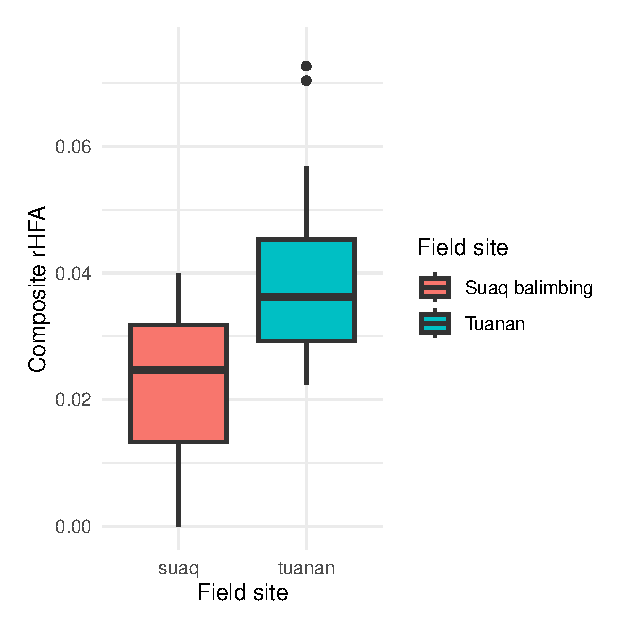
\includegraphics[width=0.6\textwidth]{Chapter2/Figs/Vector/compositefaboxplot.eps}
\caption{Variation in composite \textit{r}HFA (left) across field sites. Tuanan (Borneo) showed a significantly higher level of composite \textit{r}HFA compared to Suaq Balimbing (Sumatra), F(24,67) = 47.287, p < 0.001.}
\label{fig:Variation in composite rHFA (left) across field sites.}
\end{figure}
\section{Discussion}

The main issue with measuring fluctuating asymmetry across studies, and in particular when using photographic datasets, is accurately measuring the inherently minor variation (usually <1\% of overall trait size). This study utilised a variety of photos stretching back to 2008, so the resolution, focus, and usability varied significantly across years and individuals. These issues are exacerbated when examining arboreal primates, where there is increased distance, focal length, and variation in face orientation. However, while strict photographic selection is essential for detecting true FA, it also significantly reduces the statistical power available to detect these small deviances. This problem was exacerbated in my study due to the small sample size, 24 males across 2 sites. 

Despite only one facial HFA measure showing higher levels of FA than expected by ME, my results indicate that long-term photographic data sets can be used to examine FA. I did not observe any relationship between imaging error and total resolution, focal length, or rHFA, suggesting that there are no major issues with using older photos when examining FA over time. However, I did observe a relationship between imaging error and relative face size. This study did not scale all faces to the same size as has been done in some previous analyses by scaling the inter-pupilary distance to the same width \citep{Little.2008}. My results indicate that this is a useful step for future FA studies to minimise imaging error.

Even when scaled to the same size, the true facial size can pose a problem for FA measurements. Larger faces are more susceptible to orientation error, because minor deviations in frontal or rotational orientation are harder to assess \citep{Boulton.2013}. More studies are required to examine the impact of face size on measured FA, as currently there is no literature on the subject.

Of all of the facial LMs tested, the one that showed higher levels of FA than expected through measurement error is the outer eye tips. There are morphological reasons why this region would undergo higher levels of FA compared to other facial LMs in flanged males. The facial musculature of the orangutan forms a supporting role of the flange, in particular the M. obicularis oculi which surrounds the eye \citep{Winkler.1989}. As the flange grows, it can unevenly affect the shape of the muscle, resulting in greater FA at the outer edges of the eye tips for different individuals. As examination of non-flanged individuals was beyond the scope of this study, further examination on the differences in FA between flanged and unflanged males is needed to confirm this hypothesis. However, my results do indicate that relative facial FA can be measured on arboreal primates, subject to both a) strict photograph selection criteria, b) suitable landmark selection, and c) rigorous statistical analysis to confirm the repeatability of any measurements.

Flange measurements were significantly less repeatable and showed weaker correlation between different photographs of the same individual compared to facial measurements despite similar levels of within-photo replicability to facial LMs. There are a few potential reasons for this discrepancy. Methodologically, flange measurements may be more susceptible to measurement error compared to facial LMs. Some flanges slightly curve towards the face at the edges, and so these measurements may be more susceptible to orientation error compared to facial LMs. Additionally, as the flange has width, in instances where the face is slightly facing away from the observer, the edge of the flange will appear differently. I attempted to control for these issues with strict photo selection, however these may partially explain why these are less repeatable than facial LMs. However, there may be morphological reasons for this observed difference. The flanges are mainly made up of fat bound to fibro-fatty tissues \citep{Winkler.1989}. Under severe negative energy balance, this tissue can be used for energy under ketosis. As a result, this may cause fluctuation in flange size over the year, and if this effect is caused by nutritional deficiency, I would expect this to show a time-lagged correlation with fruit availability. I will explore this hypothesis in Chapter 3. 


\subsection{Why is FA in Tuanan greater than Suaq Balimbing?}
The results indicate that male orangutans in Tuanan experience higher levels of fluctuating asymmetry compared to Suaq Balimbing. Given the relatively minor size of the effect and that there was only one FA measure where the FA exceeded ME, it is important not to overstate the significance of the results. However, there are significant ecological differences between the two sites that may contribute to the observed differences. 
Firstly, Suaq Balimbing has the highest level of consistent fruit availability compared to any other orangutan field site \citep{Singleton.2001}. Many orangutans live in forests characterised by a large variation in fruit availability, which can lead them to fall into periods of severe negative energy balance, and the unusually high productivity of Suaq shields native orangutans from the worst of these effects. This is in part due to a wider difference in soil quality between Sumatra and Borneo due to the presence of 34 active volcanoes on Sumatra, which Borneo lacks \citep{Barber.2005}.
Second, is the ecological health of each study site. Suaq Balimbing is in the Gunung leuser National Park, which has been a protected area since colonial times and formally made a national park in 1980 \citep{Singleton.2001}. There has been minimal human intrusion into the habitat and illegal logging is uncommon. However, Tuanan Research station lies within the area that was part of the now defunct Mega Rice Project that was active from 1996-1997 \citep{Erb.2018}. As a result, this area was selectively logged in the 1990s for commercial purposes before becoming a protected area in 2003, and the area is still recovering \citep{Husson.2008}. Tropical forest fragments can recover relatively quickly from low-intensity land use; however, recovery rates vary across metrics. Recovery to 90\% of old growth values for structure and species diversity can take up to 60 years, while recovery of species composition and biomass can take over 120 years \citep{Poorter.2021}. As such, the altered community composition of the forest may exacerbate existing periods of negative energy balance due to the diminished diversity of food sources. 
Adding to this is the asymmetric impact of fires in these two communities. Borneo has experienced multiple large-scale fires, most famously the 1997 fires across 0.73Mha of forested peatland, which released between 0.81 and 2.57Gt of carbon into the atmosphere \citep{Page.2002}. These fires are made more common due to the impacts of global change and climate change, in particular the increase in the strength of El niño events; and land use change over the areas burnt \citep{Collins.2019, Siegert.2001}. These fires are part of a dangerous positive feedback loop, as previous studies have indicated that recently logged forest fragments suffer more severe damage during fire outbreaks \citep{Siegert.2001}. Additionally, areas that have recently burnt are more likely to burn again soon due to the large amount of dead flammable wood left over from large burns \citep{Cochrane.1999}. Tuanan has undergone multiple burns, including the 1997 event and most recently from March 2015 to January 2016; whereas in contrast, no fires have been recorded at Suaq Balimbing. Studies since the 2015 outbreak have indicated that fire has significant direct and indirect negative impacts on orangutans. Exposure to hazardous concentrations of \(PM_{10}\) particulate matter decreases the daily distance travelled and increases fat catabolism \citep{Erb.2018}. The secondary effects of fires are severe reduction in fruit availability, following a prolonged smoke cover period causing significantly lower overall fruit availability compared to regular annual decreases, which also causes decreased movement and increased fat catabolism \citep{Ashbury.2022}.
Given the data set of exclusively flanged males, it is difficult to distinguish the causes of the observed differences in FA between the two sites; however, future studies in the area could establish the impact of the fire on juveniles and infants by examining facial FA before and after the fire.

In summary, my results highlight the use of historic data sets for measuring facial FA and establishing differences across populations, subject to strict selection criteria, suitable landmark choice, and large sample sizes.

\nomenclature[z-DI]{DI}{Developmental Instability}
\nomenclature[z-FA]{FA}{Fluctuating Asymmetry}
\nomenclature[z-HFA]{HFA}{Horizontal Fluctuating Asymmetry}
\nomenclature[z-VFA]{VFA}{Vertical Fluctuating Asymmetry}
\nomenclature[z-DA]{DA}{Directional Asymmetry}
\nomenclature[z-AS]{AS}{Antisymmetry}
\nomenclature[z-ME]{ME}{Measurement Error}


%!TEX root = ../thesis.tex
%*******************************************************************************
%****************************** Third Chapter *********************************
%*******************************************************************************

\chapter{Reductions in Orangutan Flange Size after Initial Development: Relationship to FAI, Antagonistic Interactions, and Age}

Male orangutans are bimature with two sexually active male morphs: the unflanged male and the flanged male. Unflanged males are similar to females in overall appearance, whereas flanged males have a larger body mass, more hair, developed throat sacs capable of making long calls, and large fatty cheek pads known as flanges. Numerous field sites have anecdotally reported the presence of flanged males with degraded flanges, which in some research has been associated with the term "past-prime". I investigated 3 potential causes of this condition by measuring flange size after initial development at two sites across multiple photographs of the same individuals and correlated these observed changes with local FAI, antagonistic interactions, and behavioural data to examine the cause of this condition. In addition, I explored the relationship between changes in individual flange size with long calls, copulations, and female association. I found that flange size deterioration is driven by age, and individuals with diminished flanges produce more long calls per day. This research suggests that maintenance of the flange size is not metabolically costly and that variance in flange size after development is likely not due to ketosis, but may be driven by age-related deterioration of muscle fibres and connective tissue that supports the structure of the flange.

\section{Introduction}
Sexual selection provides an important theoretical framework for understanding the role that inter-sexual mate choice and intra-sexual competition play on the evolution of traits, behaviours, and ecology. While in theory inter-sexual selection and intra-sexual selection apply to both sexes, in mammals due to anisogamy precopulatory intra-sexual selection typically has more impact on male-male competition, and inter-sexual selection primarily reflects female mate choice \citep{Andersson.1996}. However, how sexual selection applies to specific species must be viewed under the lens of which mating system the species has, as each mating system has associated strategies to maximise fitness \citep{Kappeler.2004}. For example, in polygynandrous mating systems, males often employ many post-copulatory evolutionary strategies to maximise the chances of successful fertilisation, including particularly adaptations to the testes and penis \citep{Ros-Santaella.2015}. For example, male mandrills have large testes in relation to their body size that increase in volume up to 25\% during the mating season \citep{Setchell.2001}. Additionally, their sperm coagulates after insemination, forming a plug that increases the chances of the individual to fertilise by decreasing the opportunities of the other for successful insemination \citep{Setchell.2016}. Similar adaptations are observed in chimpanzees, which also have large testes relative to their body weight, more than 16x larger than gorilla testes relative to their body weight \citep{Dixsonwr}. These adaptions reflect species maximising fertilisation rates under social systems where the number of matings for both sexes is less limited. However, where the number of matings is limited, sexual selection acts primarily on pre-copulatory behaviour \citep{Andersson.1996, Cassini.2020}. Therefore, to increase reproductive fitness, individuals develop strategies based on the location, attraction, and monopolisation of access to mates, and these strategies often utilise secondary sexual characteristics \citep{Kappeler.2004}. 

Secondary sexual characteristics (SSCs)  can take the form of weapons that can be used to fight for access to mates, and ornaments that are otherwise non-functional traits used to signal fitness to receptive females and to signal relative dominance to other males to prevent costly antagonistic interactions \citep{Kappeler.2004}. To be honest indicators of fitness, SSCs are energetically costly and usually an active hindrance to the survival of the individual \citep{Zahavi.1975}. Despite these high costs, the signal poses significant benefits to the signaller and receiver: for males, producing high-quality SSCs is a trade-off between maximising lifespan vs. number of matings, where a significantly reduced lifespan is a worthy trade-off for a significant increase in the number of copulations \citep{Petersen.2020b6j}. Providing the SSCs are honest fitness indicators, selective females are then able to choose mates with greater than average fitness, which can then be passed onto their offspring. These female preferences for mates with high-quality SSCs allow both the SSCs and the preference to be maintained in the population through directional selection \citep{Gomulkiewicz.1991}. 

In species that possess them, producing high quality SSCs is paramount for reproductive success, however, it is important to note that these signals only impact pre-copulatory sexual selection, and the relationships between SSCs and \textit{post}-copulatory mating success vary depending on species, and there are few universalities \citep{Setchell.2003}.  

In general, there appears to be an energetic trade-off to be made with investing in ornaments used to attract mates and relative testes size, \textit{i.e.} between pre and post copulatory mating strategies, as there is an observed negative correlation in most primates between SSC ornament size and testes size \citep{Lüpold.2019}. The theory being that a large investment in secondary sexual ornaments increases the chance of female monopolisation, there is less sperm competition and hence less of a need to invest in testes size \citep{Simmons.2017}; however, this hypothesis has a couple of flaws. Firstly, this trend is not universal and in some species high-quality ornamental SSCs are positively correlated with testes size. For example, in probosis monkeys, a study of 18 males found that nose size was positively correlated with testes size, suggesting that in some species testosterone may be a functional link between expressed SSCs and post-copulatory fitness \citep{Matsuda.2020g6t}.  Secondly, across primates there appears to be a positive correlation between canine size (which can be used as sexual ornaments) and testes size, which is contrary to the theoretical negative relationship between ornaments and testes size \citep{Lüpold.2019}. 

However, the reason for this seeming contradiction may be due to the practicalities of monopolising access to mates. While the best way to maximise fitness under sexual selection theory is to monopolise access to multiple females,  when this is not possible, the next best strategy is to maximise the number of copulations \citep{Setchell.2016}. Weapons have the advantage of being used as indicators of fitness during male-male competition and to be used for coercive mating. Furthermore, purely ornamental signals of fitness are generally metabolically costly to maintain, as well as to produce; while canines are metabolically costly to produce, their metabolic maintenance may be significantly lower or use different resources to maintain compared to SSC ornaments \citep{Lüpold.2019}. 

\subsection{Testosterone, cortisol, hierarchy stability and dominance}

In diverse primate taxa, testosterone plays a crucial role in the development and maintenance of male secondary sexual characteristics (SSCs), with variations in the hormone's effects observed across species. Chimpanzees, for example, show a robust correlation between elevated testosterone levels and the manifestation of SSCs such as larger body size, and increased dominance \citep{Dixson}. Likewise, mountain gorillas display notable differences in testosterone levels between dominant silverback males and subordinate males \citep{Robbins.2004}, with silverbacks developing significant muscle mass, larger body size, and distinctive silver hair. Long-tailed macaques present another example, where dominant males with higher testosterone levels exhibit well-developed canine teeth and increased aggression during mating season \citep{Girard-Buttoz.2014}.

To better understand the role of testosterone in SSC development, it is essential to consider the challenge hypothesis. This hypothesis posits that testosterone levels in male animals are tightly regulated, primarily increasing in response to social challenges such as male-male competition, territorial disputes, and mate guarding \citep{Wingfield.1990}. According to this hypothesis, testosterone levels should rise during periods of social instability or competition and decrease during social stability when the costs of high testosterone outweigh the benefits. The challenge hypothesis specifically contends that variations in testosterone levels during the breeding season correlate more closely with male aggression in reproductive contexts than with changes in reproductive physiology \citep{Wingfield.2020}. Therefore, assessing the influence of testosterone on the development of SSCs requires acknowledging additional factors, such as species-specific social structures, mating systems, and ecological pressures, which also modulate the expression of these traits and their relationship with testosterone levels.

In some primates, circulating testosterone levels are directly influenced by the dominance of the individual within their social hierarchy, rather than being a predictor of future dominance. Basal testosterone and cortisol levels in individually housed cynomolgus monkeys (\textit{Macaca fascicularis}) did not predict eventual social rank, however, cortisol levels after social housing could predict whether an individual would become subordinate and basal testosterone levels were higher in dominant males \citep{Czoty.2009}. In bearded capuchins, alpha males have higher levels of circulating testosterone than their peers, even under unstable dominance hierarchies \citep{Mendonça-Furtado.2014}. Similar relationships can be seen in great apes.  In chimpanzees, even when controlling for age, circulating testosterone is positively correlated with both dominance rank and aggression rates against other individuals \citep{Anestis.2006}. But this pattern is not universal, in bonobos there is no correlation between dominance rank and testosterone levels in either sex \citep{Sannen.2003}. This divergence in the role of testosterone in these closely related species can be attributed to their different social structures and mating systems, and cautions overly simplistic interpretations of the causative role of testosterone on dominance or mating success.

Cortisol also plays a significant role in dominance in several primates. In some species, high-ranking individuals exhibit elevated cortisol levels due to the increased stress associated with maintaining their dominant status and engaging in aggressive interactions. In male chimpanzees, dominant individuals have been found to exhibit higher levels of cortisol compared to subordinates, particularly in situations of social instability and increased competition \citep{Muller.2004}. Similarly, in rhesus macaques, dominant males have been reported to display elevated cortisol levels, which has been associated with the increased frequency of agonistic encounters and the necessity of maintaining dominance rank \citep{Sapolsky.1992}. In contrast, other primate species demonstrate an inverse relationship between dominance rank and cortisol levels, with subordinate individuals exhibiting higher cortisol levels due to stress induced by their lower social status. For example, in Assamese macaques, subordinate males have been observed to display elevated cortisol levels, which has been linked to increased harassment and social subjugation experienced by these individuals \citep{Ostner.2008}. Furthermore, some primate species show more complex relationships between cortisol levels and dominance rank, wherein the association is influenced by factors such as social stability and group dynamics. For instance, in olive baboons, dominant males have been found to exhibit higher cortisol levels during periods of social instability, while subordinate males display elevated cortisol levels under stable social conditions \citep{Gesquiere.2011}. Generally, dominant males are predicted to undergo more stress under unstable dominance hierarchies than subordinant males, while the opposite is predicted under stable dominance \citep{Kappeler.2004}. However, in practice these predictions vary according to species, reflecting the diversity of the primate family. 

Regardless of the dominance system, the normal impacts of psycho-stress on individuals is usually a temporary condition as a result of an acute event, which leads to increases in cortisol and epinephrine \citep{Edes.2017}. These effects return to normal when the cause of the stress is removed, however under continuous social stress such as the stress of dominant male in a unstable dominance hierarchy this can lead to impacts on long term health \citep{Maestripieri.2011}. The cumulative effect of stress on health outcomes and disease is known as allostatic load, and these impacts are just starting to be examined in captive primates. In captive zoo-housed lemurs, smaller groups sizes, frequent group changes and cumulative time spent indoors all correlated with increased allostatic load \citep{Seeley.2021gr8}. In captive African great apes, age is significantly correlated with increased allostatic load; and notably in captive chimpanzees and western lowland gorillas, cumulative stressful events are also correlated with increased allostatic load \citep{Edes.2016,Edes.2023}. While the nature of the relationship between an individuals allostatic load and degradation of SSCs has not yet been explored in great apes, if SSCs are unbiased indicators of fitness elevated, presence of these biomarkers may be part of the mechanism that leads to degradation of the quality of the signal produced by the trait.


\subsection{Sexual selection and orangutans}

Orangutans are the only great apes to live outside of Africa \citep{Wich.2008}. Now only located in Sumatra and Borneo, they live in tropical forests characterised by their large variability in fruit production. Uniquely among great apes, male orangutans are bimature, meaning there are two sexually active male morphs: the unflanged male and the flanged male \citep{Prasetyo.2021}. Unflanged males are similar to females in body size and overall appearance, while flanged males have a larger body mass, more hair, developed throat sacs capable of making long calls and large fatty cheek pads, known as flanges \citep{Knott.2008}. Due to their semi-solitary social system and consequential difficulties in gathering large behavioural data sets, it's unclear whether orangutan SSCs are unbiased indicators of fitness, or even whether they all reflect the same measure of fitness. 

Male orangutans experience intense sexual selection, especially male-male competition and female choice. While flanged males are broadly tolerant of unflanged males, and unflanged males are largely tolerant of each other; interactions between two flanged males, while rare, are invariably antagonistic, and often result in significant injuries such as fingers or upper lip being bitten off \citep{Setia.2008}. Given that females do not advertise ovulation, have long inter-birth intervals, and the species' semi-solitary social structure, these factors are predicted to increase the intensity of male-male competition and suggest that monopolisation of females is the best strategy for maximising the number of offspring \citep{Galdikas.1985, Kappeler.2022}. However, interestingly in practice, aggression between flanged males appears to decrease in the presence of a female, suggesting that aggression rates may be due to highly overlapping ranges, as opposed to access to females \citep{Dunkel.2013,Marty.2015}.

Female orangutans show a strong mate preference for flanged males, resulting in the two morphs developing alternate mating strategies. Flanged males utilise a "call and wait" strategy, as their developed throat sacs enable flanged males to produce long calls, distinct vocalisations that travel up to 1.3km in the forest depending on the terrain \citep{Spillmann.2016}. Other flanged males do not significantly approach or move away from these calls, and unflanged males retreat; while females move towards the source of the call \citep{Setia.2007}. These calls have dual purposes: attracting females and acting as a spacing mechanism for flanged males \citep{Spillmann.2010}. When females do arrive, flanged males can enter consortships with them (which is more common during masting events), where they travel and nest together for a few days while sporadically mating \citep{Atmoko.2008saj}. 

Unflanged males, lacking the ability to make long calls, instead utilise a "silent searching" strategy: roaming around the forest in active search for females, and when they find them often resort to forced copulation, which is uncommon among great apes \citep{Atmoko.2008saj, Utami.2002km8}. 

Among flanged males, the most successful mating strategy varies depending on location. For example, Suaq Balimbing in Sumatra due to its high primary productivity and year-round fruit availability is capable of supporting the highest density of wild orangutans in the world, and these ecological factors support local dominant male and stable dominance hierarchies. However, in Tuanan, a site in central Kalimantan, where fruit and food availability is much more variable and hence ranges are larger, the social structure has a much more unstable dominance hierarchy, and some flanged males do employ the "search and find" mating strategy \citep{Kunz.2023}. Hence, the evolutionary stable strategy for male individuals depends on the level of monopolisation of females, and consequently sites with higher levels of monopolisation have a higher ratio of unflanged males to flanged males.

\subsection{Flanges and orangutans}

Flanges are the most conspicuous SSC that male orangutans develop. Physiologically, they are primarily formed of fat deposits bound to fibro-fatty tissues \citep{Straus.1942}. The initial growth of flanges begins with the other SSCs during the bimaturism process, which usually completes within 3 years, however during bimaturism antagonistic interactions from flanged males causes social stress which has been shown in some cases to arrest the bimaturism process \citep{Prasetyo.2021}. The exact trigger for bimaturism is unknown, however it is known that the triggering is not linked to nutritional availability, as individuals under nutritional stress can still go through bimaturism \citep{Prasetyo.2021}. There appears to be social correlates of the triggering of bimaturism, as the same social stresses that can arrest the growth of SSCs also appear to inhibit their development \citep{Dunkel.2013xnm}. These findings help explain the varying rates of bimaturism between sites and species. 

Overall flange size, shape and symmetry varies between individuals, sites and species, however their reflection of dominance relative to other flanged males, and indication of overall fitness is unknown \citep{Prasetyo.2021, Wich.2019}. There are observations from field stations in Borneo and Sumatra that have noted a reduction in flange size after their development \citep{Knott.2009b, Dunkel.2013}. This gives the flanges a shrivelled or deflated appearance. \citet{Knott.2009b} asserts the wider presence of a "past-prime" orangutan condition, with severely shriveled flanges which are subordinate to flanged males. 
Previous hypotheses have suggested that this may be associated with old age or nutritional deficiency, however any investigations into the cause of this condition have not yet been published \citep{Galdikas.1978,Knott.2008}. Nor has there been an attempt so far to quantify the magnitude of these changes.

As of yet, it remains unknown whether this condition is a physiological change that comes about after an individual has met a threshold condition, or whether there is larger variation in orangutan flange size after initial growth along a continuous spectrum. Given the physiology of the flange, and the metabolically costly nature of secondary sexual characteristics, maintaining a consistent size of these cheek pads may become compromised under specific environmental or individual conditions. A few possibilities as to the cause of this condition are:

\subsubsection{Nutritional deficiency as a cause of the "past-prime" condition}
Nutritional deficiency is a possible cause of this condition as orangutans live in forests characterized by irregularity and unpredictability in fruit production \citep{Morrogh-Bernard.2011}. Fruit production peaks approximately every 4 years in Sumatra during masting events triggered in part by the El Niño-Southern Oscillation phenomenon \citep{Wich.2000}. However when fruit is scarce, orangutans have been documented to have greatly reduced energy intake and fall into negative energy balance \citep{Erb.2018}. While fruit provides significantly greater energetic returns than fallback foods such as bark or pith, orangutans appear to have developed physiological adaptations to buffer against negative energy balance. Evidence of ketosis in wild orangutans is only seen during periods of low fruit availability, suggesting efficient energy storage as fat during periods of high fruit availability \citep{Erb.2018, Knott.1998}. 

However, for their body mass flanged males consume less calories than unflanged males, which may be due to unflanged males showing increased roving behaviour compared to the flanged male \citep{Vogel.2017}. Given that flanges morphologically are primarily adipose tissue, under ketosis this adipose may be burned for additional energy. Hence under this hypothesis, the flange serves as an honest signal of energetic balance for the purposes of mating, and the ability of the signaller to buffer against environmental change. 

\subsubsection{Antagonistic social stress}
However the social stresses that arrest and inhibit development may also be the cause of this condition. Antagonistic interactions have been shown to spike cortisol levels, which are correlated with inhibited flange development \citep{Thompson.2012}. These interactions can be indirect, as in both unflanged males and flanged males, hearing another flanged males long call causes an increase in cortisol levels \citep{Prasetyo.2021}. Both of these causes are somewhat secondary, and trigger activation of hormonal pathways for development of flanges and other associated SSCs. The understanding of the hormonal processes driving bimaturism are murky due to the semi-solitary social structure of orangutans, as well as their arboreal lifestyle making measurement difficult. Current evidence is inconclusive, however it does appear that testosterone is correlated with delayed flange development in captive orangutans \citep{Thompson.2012, Muller.2017}. However, captive orangutans' hormonal profiles are significantly different to wild populations, for example captive populations experience significantly higher levels of cortisol, and reduced levels of testosterone \citep{Prasetyo.2021}. However the same hormonal processes that drive initial flange development, may also impact the maintenance of these SSCs, and in turn interact with some of the other potential causes, as it's been noted that variation in feeding rates appears to drive differences in cortisol levels in some field sites \citep{Prasetyo.2021}.

\subsubsection{Relative age}
In polygynous and polygynandrous species, senescence is experienced more severely by males compared to females, due to a combination of evolutionary and early life factors \citep{Graves.2007}. Species with high levels on intra-sexual competition have a higher risk of mortality, which can lead to a reduction in the selection against deleterious mutations which can impact senescence \citep{Williams.1957}. However these factors are complicated by individual history of the individual, as early life adversity can impact the onset and severity of senescence \citep{Beirne.2015} Additionally, age may act as a synergistic factor which increases the impact of ecological stressors on individuals. Older individuals may have more difficulty accessing or processing food sources, which may in turn impact their health over time. Previous research has indicated correlations between maintained low dominance ranking and chronic psycho-social stress in rhesus macaques \citep{Maestripieri.2011}. These impacts then cause an allostatic load on the individual which can increase the probability of age related cognitive decline, mortality risk and cardiovascular disease. These results indicate a synergistic interaction between age and antagonistic interactions, however social stress in primates depends heavily on the stability of the dominance hierarchies of the chosen species and habitats \citep{Czoty.2009, Mendonça-Furtado.2014, Muller.2004}. 


\subsubsection{Correlations with long call behaviour}
If one of the aforementioned factors does correlate with a decrease in overall flange size, then the same metabolic pathways that impact flange size may have impacts on other associated SSCs. Male orangutans develop their complex throat pouches during bimaturism, and development can be arrested in the same way that flange development via the same psychoendoneurological mechanisms \citep{Prasetyo.2021}. Long calls contain contextual clues about the individual producing them and is the first way females are able to assess the quality of flanged males \citep{Spillmann.2010}. These calls can be made spontaneously or in reaction to hearing another long call as a method of confrontational assessment \citep{Spillmann.2016}. While previous studies have not seen a relationship between fruit availability and long call rates (suggesting they are not energetically costly to produce), individual body condition may still impact the duration or composition of long calls during periods of low fruit availability \citep{Spillmann.2016}. Additionally, age related muscle deterioration may reduce the the duration or number of pulses in a long call.

\subsubsection{Impacts on mating behaviour}
If relative flange quality is a SSC used to discern mate choice, then we would expect individuals with a reduction in overall flange size to experience negative outcomes when associating with females. In particular, females will either reduce the time spent in association with these flanged males during fertile periods, or reduce time spent in association with them altogether. Additionally, as females will not willingly copulate with individuals of poor quality we would expect to see either a reduction in overall copulation rates per hour of female association or an increase in the proportion of copulations that are forced.

\subsection{Study Aims}
This study aims to investigate the underlying causes impacting the observed variation in orangutan flange sizes and shapes after their initial development, and what life history or ecological factors are correlated with these changes. Additionally I wish to explore correlations between a change in flange size with long call rates, composition and duration; as well as impacts on mating success. 

Given the different ratios of flanged males to unflanged males/females between sites, the adipose content of flanges and the differing ecologies of the two sites, I predict:

\begin{enumerate}
    \item   Temporary reduction in flange size, where present, will follow periods of significant decreases in fruit availability.
    \item Antagonistic male-male interactions, including fights, will also cause flange size reduction due to the psychoendocrinilogical stress of the interaction.
    \item As decreases in overall fruit availability will lead to increases in ranging behaviour, rates of male-male interaction will also increase; causing an interactive effect between these ecological and social factors.
    \item Due to ecological and population differences between sites, I predict these effects will be seen more commonly in Tuanan compared to Suaq Balimbing.
    \item Individuals experiencing temporary reduction in flange size will produce long calls less often, or for a short period of time with fewer pulses.
    \item Individuals experiencing temporary reduction in flange size will spend fewer hours per follow day in association with females, and will have fewer proceptive copulations.
\end{enumerate}

\section{Methods}
\subsection{Study sites}
Data was collected at two field sites of high orangutan population density: Suaq Balimbing (located in Sumatra) and Tuanan (located in Borneo).

Suaq Balimbing Research Station (3°04'N, 97°26'E) is a field site located in the Gunung Leuser National Park  in south Aceh, Sumatra. Suaq Balimbing is a primary peat-swamp forest, which contains the highest density of wild orangutans in the world, with approximately 7.0 individuals/ km$^{2}$, supported by the availability of fruits year-round and comparative lack of anthropogenic disturbance \citep{Fox.2004, Schaik.1995}.

Tuanan Orangutan Research Project (2°09'S, 114°26'E) is located in the Mawas Reserve in Central Kalimantan, Borneo. Tuanan Research Station is located in a section of peat-swamp forest, and contains approximately 4.5 individuals/km$^{2}$, and the density of orangutans is among the highest in Borneo \citep{Husson.2008} . The site has a history of anthropogenic disturbance, including selective logging, and is increasingly suceptible to wild fires \citep{Cochrane.1999, Erb.2018}.

\subsection{Flange data}
Individuals were described as flanged, flanging or unflanged depending on their physical appearance. While the exact flanging onset remained ambiguous (as some large unflanged males might display minor cheek protrusions for multiple years due to the differential impact of socially induced development arrest) \citep{Kunz.2023}, the transition between the unflanged and flanged states was markedly distinct. Flanged males have fully developed SSCs and are capable of making long calls. Behavioural and photographic data was only used by individuals coded as "flanged".

Photographs were taken opportunistically during behavioural follows, including of associated party members. In this study due to the strict photographic requirements, all photographs were taken during focal follows of the individual studied. Since it was not possible to obtain pictures of orangutans from a fixed distance, flange size measurements taken are relative to the distance between facial landmarks (LMs) (see Chapter 2). Photographs were chosen where the orangutan is facing the camera head on, and were discarded if they were blurry, poor resolution or if any of the LMs could not be accurately placed. 

The photographs were orientated such that the middle of each pupil fell on a horizontal line, and 6 facial LMs were placed on the orangutans face. For detailed explanation of how these LMs were recorded, see Chapter 2. Two measures of orangutan flange size were used for this study.  

\begin{figure}
    \centering
    \includegraphics[width=1.0\textwidth]{Chapter3/Figs/mawasboth.eps}
    \caption{Facial LM placement on an example flanged male. Left image a) Relative flange width was estimated for each individual on a given follow day as \(  \frac{D6 \div D2}{D6\textit{max} \div D2\textit{max}}\) . Right image b) Relative flange area was calculated as the area contained within the irregular shape bounded by the points P\textit{n} using Gauss's formula}
    \label{fig:orangutanfameasures}
\end{figure}

The relative width of the flange was estimated by placing LMs on the inner tips of the eyes of each photograph and drawing a horizontal line to connect the two LMs (Figure 3.1.) This line was then extended until it reached the edge of the flange. The length (pixels) of the connecting line was divided by the inner eye distance to provide a relative measurement of flange width. To obtain comparable measurements, the relative flange width measurement was divided by the maximum recorded flange width measurement for each individual, so that each photograph has a proportional measurement of flange width between 0 and 1. Individuals with only one suitable photograph were not used for statistical analysis. This measurement of flange width was chosen due to its reliability during measurement and because of the intersection of the \textit{Mm. orbitotemporalis}, \textit{Mm. frontalis}, and \textit{Mm. zygomaticus} muscles around the eye and the high content of adipose tissue, this is the area hypothesised to be under the most pressure from my hypothesised causes \citep{Winkler.1989}. 

Relative flange area was estimated by placing 8 LMs on the orangutan's flanges by bisecting facial LMs as shown in Figure 3.2.  The area of the irregular shape enclosed by these coordinates was calculated using Gauss's area formula. This area was then divided by the square of the inner eye distance to provide a relative measure of flange area. Comparable measurements were obtained using the same method as for flange width, by dividing each image's relative flange area by the maximum recorded value for that individual. Images were rejected if they did not contain all 8 flange LMs. 

\begin{figure}
\centering
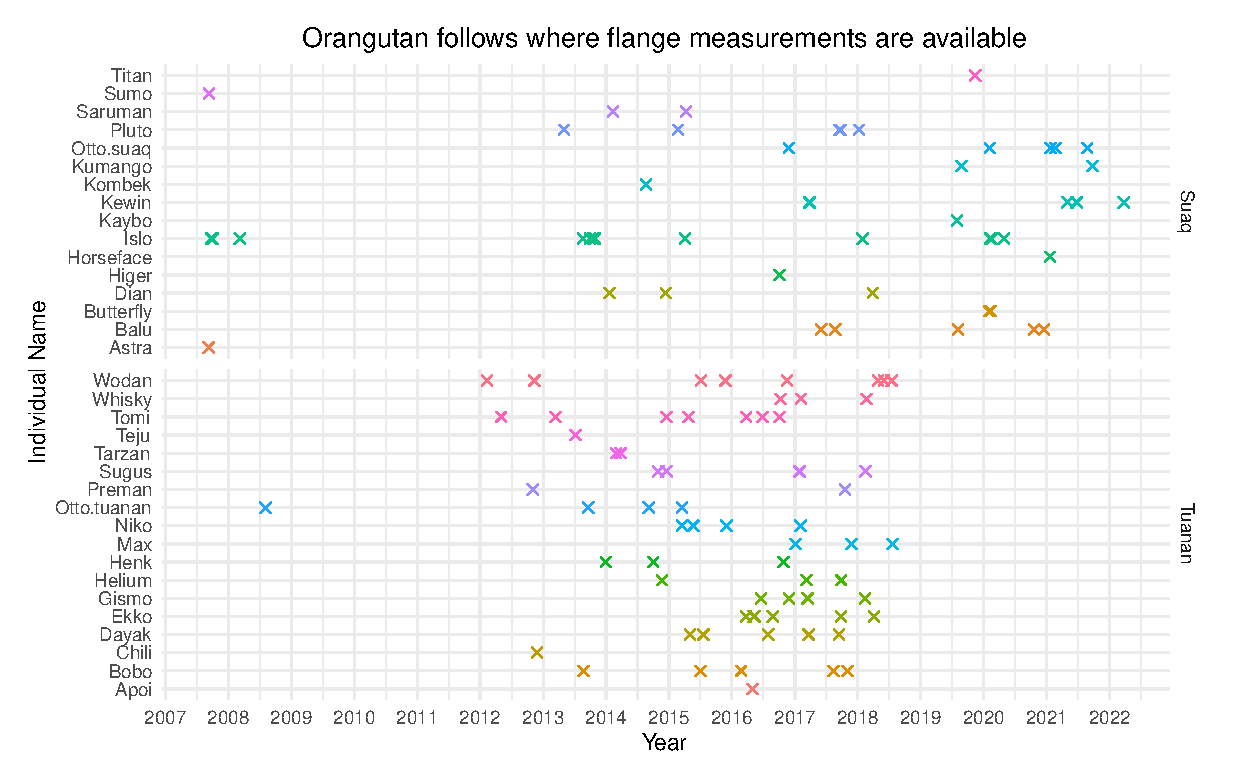
\includegraphics[width=1\linewidth]{Chapter3/Figs/sightings_plot.eps}
\caption{Timeline (x-axis) illustrating days where a flanged male was followed (ie focal individual), and the resulting photgraphs were of sufficient quality to obtain relative flange measurements at Suaq Balimbing and Tuanan. Individuals with only one suitable photograph were not used for analysis.}
\label{fig:orangutan_sightings_with_measurements}
\end{figure}

\subsection{Behavioural data}
Behavioural data was collected during daily nest-to-nest behavioural follows using 2 minute instantaneous focal sampling using an established protocol \citep{OU_methods}. Across both sites, a total of 993 focal follows hours were matched to a follow day where a reliable flange measurement was available. At Suaq, a total of 372 hours of focal follow data were used, collected between 2007 and 2021. At Tuanan, a total of 621 hours of focal follow data were used, collected between 2007 and 2018. During each follow, the number of long calls produced by the focal follow subject were noted. The duration and number of pulses per long call were also noted. In each follow the number of long calls emitted by another individual (who was not the focal follow) was also noted.

The identity of each focal subject was identified primarily via comparison of daily photographs with a known database of individuals at each site. In some cases identification was also confirmed using genetic analysis of faecal samples. Individual identification is difficult in both sites as roving males frequently leave the study area and may not appear again for many years \citep{Kunz.2023,Mörchen.2023}. For that reason, identification was only confirmed without genetic verification if multiple independent observers reported them as the same individual.

Relative age was calculated by subtracting the date of the earliest known photograph of an individual from the date the studied photograph was taken. Individuals were excluded from analysis if they were observed within the study area in an unflanged state to prevent systematic biases.

Antagonistic interactions were recorded for each behavioural follow and the type of interaction from fleeing to fights were all scored equally. For each flange measurement date, the cumulative number of antagonistic interactions observed at that point in time for that individual was noted. While this introduces a potential bias as the value will always increase or stay the same for later photographs, I used the cumulative number of antagonistic interactions, as opposed to a rate per day to account for the compounding allostatic load of cumulative antagonistic interactions; and to account for potential delays in response to the antagonistic interaction.

As direct antagonistic interactions have only been directly observed in Tuanan, and lacking sufficient data to analyse long call confrontational measures of assessment across both sites \citep{Spillmann.2016}, all models including antagonistic social interactions as a factor focus only on the Tuanan site utilise observed antagonistic interactions. To assess potential multicollinearity as cumulative interactions accumulate over time, both Pearson's correlation and the Variance Inflation Factor (VIF) were calculated. The results indicated a significant correlation between relative age and antagonistic interactions (Pearson's r = 0.304, t = 2.692, p-value = 0.009), implying some degree of linear association between these two variables. However, despite this significant correlation, the VIF of 1.12 is well below the commonly used threshold of 5, suggesting that the level of multicollinearity is unlikely to disrupt the stability or interpretability of a regression model based on these variables. Therefore, while a certain degree of correlation is present, it does not translate into a problematic level of multicollinearity.

Association with females was measured by the total hours spent within 50m of females. This figure was cumulative per female, so if 2 females were in association with the focal for 1 hour, this would be coded as 2 hours of female association. As the population density and average hours of female association was significantly higher at Suaq compared to Tuanan, for some analyses the hours of female association was z-transformed (zAssocH). Copulations are relatively rare to observe at Suaq and Tuanan \citep{Kunz.2023}, so given the sample size all successful (achieved intromission) copulations were coded the same (Cop) to assess the number of copulations per hour of female association with no attempt made to distinguish between forced and receptive copulations. 

Long call data was collected opportunistically during focal follows. For each long call, the number of pulses and duration was estimated, however, these additional elements were not available for every long call in the data set. I then averaged the duration of long calls per follow day, and averaged the number of pulses per long call per follow day. As long call rates are hypothesised to be impacted by rainfall but the exact timing of rainfall in comparison to the long call was unknown, the number of hours of rainfall for each follow day was noted and added as a fixed effect in models examining long call behaviour.

\subsection{Ecological data}
Phenological data on fruit availability was taken monthly at both sites throughout the entire study period. The Fruit Availability Index (FAI) was calculated as the percentage of trees with fruits across all surveyed trees in the study site. As fruit availability is higher in Suaq, and the number of trees surveyed differed for each site (Approximately 1000 at Suaq, and approximately 1500 at Tuanan),  for some analyses the FAI was z-transformed. Where the z-transformation value has been used the variable will be written as zFAI. To account for a time lag between the impact of FAI and the effect on flange size, the measure of FAI chosen was average FAI for the current month, and the preceding two months using the \textit{dplyr} package \citep{dplyr.2023}.

As rainfall appears to have an impact on the number of vocalisations produced by vocal rainforest primates \citep{Clink.2020, Kunz.2023}, I took steps to account for the presence of rain on long call rates. As each long call could not be reliably matched to the weather at a particular time, the total hours of rainfall that follow day was included as an explanatory variable for some analyses.

\begin{figure}
\centering
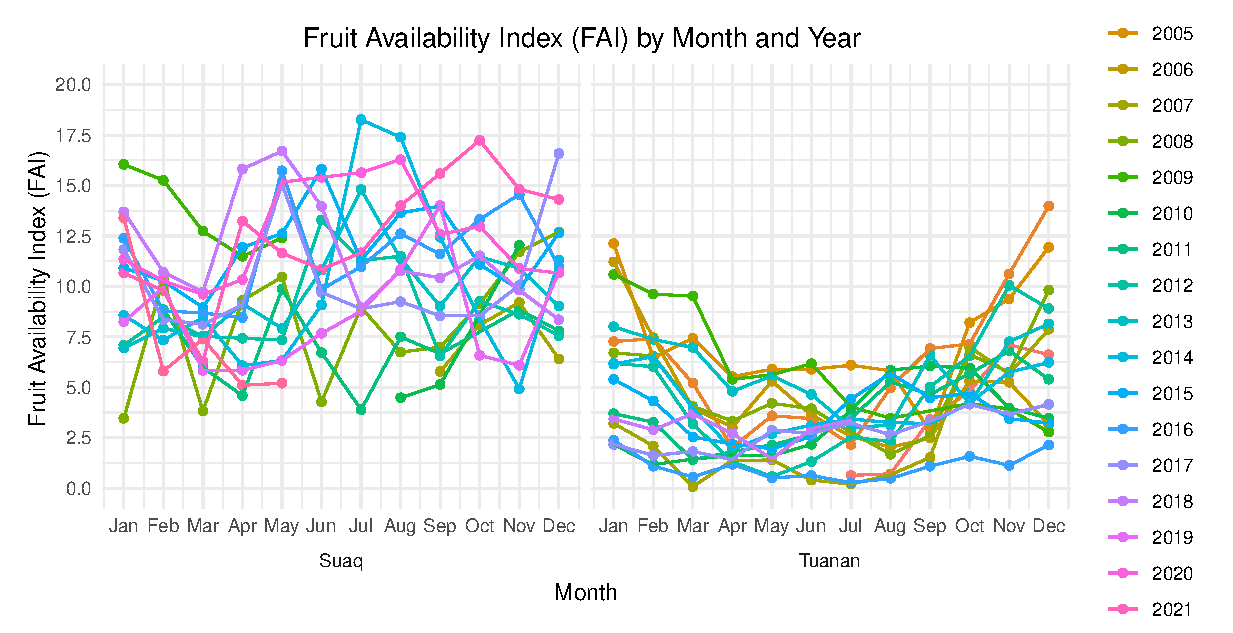
\includegraphics[width=1\linewidth]{Chapter3/Figs/plot.eps}
\caption{Fruit Availability Index (FAI) by month of the year. FAI was calculated as the percentage of trees with fruits across all surveyed trees in the study site. The left plot shows FAI in Suaq (Sumatra), and the right plot shows FAI in Tuanan (Borneo). }
\label{fig:FAI_by_month_between_Suaq_and_Tuanan}
\end{figure}

\subsection{Analysis}

I investigated the impact of the Fruit Availability Index (FAI), study site, and individual orangutans on the relative flange size in orangutans with Gaussian linear mixed-effects models (LMMs) using the \textit{lme4} package in R \citep{Bates.2015}. The model was fit using restricted maximum likelihood (REML), and the significance of the fixed effects was assessed using Satterthwaite's method for approximating degrees of freedom. The model included the fixed effects of: years since first seen, FAI (averaged over three months), study site, and the interactive effect between FAI and study site. Individual orangutan identity was included as a random effect. 

As antagonistic interactions have only been observed in Tuanan, and in absence of a robust proxy, LMMs which examined the impact of antagonistic interactions were only run on the Tuanan measurements. These LMMs included the fixed effects of Years since first seen, FAI (averaged over three months), antagonistic interactions, the interactive effect between antagonistic interactions, and FAI (averaged over three months). Individual orangutan identity was also included as a random effect. 

Null models were created for each model with an effect structure of \(Response ~ 1 + (1|Name)\). All models were run twice, with the response variable being either relative flange width, or relative flange area. Models were evaluated to the null model using Akaike Information Criterion (AIC) with the change in AIC listed next to each model. 

Following the fitting of the models, I examined the normality of residuals and homoscedasticity to validate the model's fit. This was achieved via visual inspection of Q-Q plots and residual versus fitted value plots. Additionally, the variance inflation factor (VIF) was calculated to assess multicollinearity among the predictors. A high VIF for any predictor variable suggests that it is highly collinear with the other predictors, and may necessitate the removal of that variable from the model. 

To assess the potential impact of reduced flange size on mating behaviour and associated long call behaviour, I used Generalized linear mixed models using the \textit{glmTMB} package in R \citep{Brooks.2017}. Continuous response variables, including average duration of long calls and number of hours in association with a female were examined using Gaussian linear mixed-effect models. Count based response variables, including number of long calls per follow day, number of pulses per long call, and number of copulations were assessed with Poission linear mixed-effect models.

All models were tested for over‐dispersion. If data in a model with Poisson distribution revealed over‐dispersion, I conducted negative binomial GLMMs as a robust alternative. All models were created with the nested random intercept of (1|Name/Year/Month), however in the instance of singularity errors, the random intercept was reduced to (1|ID).

All plots were produced using \textit{ggplot2} and \textit{ggeffects} was used to illustrate model effects. All statistical tests are two-tailed unless otherwise stated, and statistical analysis was performed in R version 4.3.0 (\citep{R.2018, Wickham.2011, Lüdecke.2018}. 

\subsection{Ethical note}
Behavioural data collection was strictly observational and non-intrusive. There was no engagement between observers and the wild orangutans; a minimum distance of 10 metres was maintained to ensure the subjects' natural behaviour remained uninfluenced. The procedures for data gathering were in line with Indonesia's legal stipulations and received approvals from the Indonesian State Ministry for Research and Technology (RISTEK), the Directorate General of Natural Resources and Ecosystem Conservation - Ministry of Environment and Forestry of Indonesia (KSDAE-KLHK), the Ministry of Internal Affairs, Indonesia, the Nature Conservation Agency of Central Kalimantan (BKSDA), and the Balai Besar Taman Nasional Gunung Leuser (BBTNGL).

\section{Results}
\subsection{Life history and ecological impacts on relative flange size}
To examine the impact of ecological factors on relative flange size, 8 linear mixed models were fitted by REML using Satterthwaite's method for t-tests. Each model was run twice with the response variable changing between Relative Flange Width and Relative Flange Area. 

Our first pair of models were run on measurements collected from both field sites on the explanatory variables of relative age, the average FAI of the preceding 3 months, field site (as a factor) and an interactive effect between FAI and the field site.

The interaction between zFAI average over three months and study site was not significant (Estimate = 0.046850, p-value = 0.236497), suggesting that the effect of zFAI on relative flange size does not significantly differ between the study sites. As such the model was re-run leaving out this interactive effect.

\begin{table}
    \centering
    \resizebox{\textwidth}{!}{%
    \begin{tabular}{l l r r r r r}
    \hline 
    \multirow{1}{*}{\textit{Response}} & \multirow{1}{*}{\textit{Fixed effects}} & \multirow{1}{*}{\textit{Estimate}} & \multirow{1}{*}{\textit{Std. error}}  & \multirow{1}{*}{\textit{df}} & \multirow{1}{*}{\textit{t-value}}  & \multirow{1}{*}{\textit{p-value}}\\ 
    \hline
   \textbf{1. Proportion of eye flange width} & \textbf{Intercept} & \textbf{1.003} & \textbf{0.039} & \textbf{86.739} & \textbf{25.482} & \textbf{< 0.001}\\

      & \textbf{Years since first seen} & \textbf{-0.009} & \textbf{0.002} & \textbf{43.240} & \textbf{-3.730} & \textbf{0.001}\\

    N = 111, $\Delta$ AIC = 26.19 & zFAI (3 month average) & -0.052 & 0.030 & 99.736 & -1.736 &  0.086\\
 
     & Field Site (Factor) & -0.022 & 0.045 & 78.292 & -0.489 &  0.626\\

    & zFAI (3 month average) : Field site (As factor) & 0.047 & 0.039 & 103.255 & 1.191 &  0.236\\
    \cline{2-7}
        & \textit{Random effects} & & & & \textit{Variance} & \textit{Std. dev.}\\
    \cline{2-7} 
    & Name (Intercept) & & & & 0.002 & 0.043 \\
    & Residual & & & & 0.006 & 0.075 \\
     \hline 
   \textbf{2. Proportion of flange area} & \textbf{Intercept} & \textbf{0.892} & \textbf{0.121} & \textbf{68.527} & \textbf{7.340} & \textbf{< 0.001}\\

     & Years since first seen & -0.005 & 0.007 & 28.726 & -0.702 & 0.488\\

   N = 81, $\Delta$ AIC = 25.846  & zFAI (3 month average) & -0.117 & 0.095 & 73.298 & -1.236 &  0.220\\
 
    & Field Site (Factor) & 0.024 & 0.138 & 67.965 & 0.171 &  0.865\\

    & zFAI (3 month average) : Field site (As factor) & 0.216 & 0.123 & 75.824 & 1.753 &  0.084\\
    \cline{2-7}
        & \textit{Random effects} & & & & \textit{Variance} & \textit{Std. dev.}\\
    \cline{2-7} 
    & Name (Intercept) & & & & 0.009 & 0.092 \\
    & Residual & & & & 0.040 & 0.200 \\
     \hline 
\end{tabular}
    }
    \caption{Results of the LMM examining the impacts of social and ecological factors on the flange size response variables across both field sites.. The fixed effects used were relative age, 3 month average FAI, field site (as a factor) and an interactive effect between 3 month average FAI and field site. This model included a random effect of an individual.
    Formula used was: \(Response \sim YearsSinceFirstSeen + FAI (3MonthAverage) * FieldSite (as.factor) + (1 | Name)\) }
\end{table}
This pair of models showed a significant result. With relative flange width as the response variable (Model 3, Table 3.2), this model revealed a significant effect of years since first seen (relative age) on relative flange width (Estimate = -0.009, p-value < 0.001). 
There was no overall impact of zFAI on relative flange width across sites, nor was a significant difference in flange width observed between the two sites (Estimate = -0.052, p-value = 0.086).

In contrast, where the proportion of flange area was the response variable (Model 4, Table 3.2), I did not find a significant impact of years since first seen on flange size (Estimate = -0.005, p-value = 0.4881). Similar to the all-sites-width model, there was no observed overall relationship between 3 month average FAI and flange size (Estimate = -0.117, p-value = 0.220).

There was no observed significant relationship between field site and relative flange width or area in either model 3 or 4 (Estimate = 0.111, p-value = 0.371; Estimate = 0.024, p-value = 0.865).

\begin{table}
    \centering
    \resizebox{\textwidth}{!}{%
    \begin{tabular}{l l r r r r r}
    \hline 
    \multirow{1}{*}{\textit{Response}} & \multirow{1}{*}{\textit{Fixed effects}} & \multirow{1}{*}{\textit{Estimate}} & \multirow{1}{*}{\textit{Std. error}}  & \multirow{1}{*}{\textit{df}} & \multirow{1}{*}{\textit{t-value}}  & \multirow{1}{*}{\textit{p-value}}\\ 
    \hline
   \textbf{3. Proportion of eye flange width} & \textbf{Intercept} & \textbf{0.990} & \textbf{0.030} & \textbf{71.427} & \textbf{33.086} & \textbf{< 0.001}\\

     & \textbf{Years since first seen} & \textbf{-0.010} & \textbf{0.002} & \textbf{56.544} & \textbf{-4.465} & \textbf{< 0.001}\\

   N = 111, $\Delta$ AIC = 18.371  & zFAI (3 month average) & -0.015 & 0.017 & 113.86 & -0.887 & 0.377\\
 
      & Field Site (Factor) & -0.005 & 0.039 & 81.637 & -0.137 & 0.891\\
    \cline{2-7}
        & \textit{Random effects} & & & & \textit{Variance} & \textit{Std. dev.}\\
    \cline{2-7} 
    & Name (Intercept) & & & & 0.002 & 0.047 \\
    & Residual & & & & 0.005 & 0.074 \\
     \hline 
   \textbf{4. Proportion of flange area} & \textbf{Intercept} & \textbf{0.805} & \textbf{0.098} & \textbf{48.057} & \textbf{8.203} & \textbf{< 0.001}\\

      & Years since first seen & -0.010 & 0.006 & 38.823 & -1.479 & 0.147\\

    N = 81, $\Delta$ AIC = 20.762 & zFAI (3 month average) & 0.036 & 0.054 & 80.933 & 0.668 & 0.506\\
 
    & Field Site (Factor) & 0.111 & 0.124 & 63.613 & 0.900 & 0.371\\

    \cline{2-7}
        & \textit{Random effects} & & & & \textit{Variance} & \textit{Std. dev.}\\
    \cline{2-7} 
    & Name (Intercept) & & & & 0.011 & 0.105 \\
    & Residual & & & & 0.039 & 0.199 \\
     \hline 
\end{tabular}
    }
    \caption{Results of the LMM examining the impacts of social and ecological factors on the flange size response variables across both field sites.. The fixed effects used were relative age, 3 month average FAI, field site (as a factor). This model included a random effect of an individual.
    Formula used was: \(Response \sim YearsSinceFirstSeen + FAI (3MonthAverage) + FieldSite (as.factor) + (1 | Name)\) }
\end{table}

The next pair of models were solely run on the data acquired from Tuanan, which remains the unique site where antagonistic interactions have been directly observed and recorded. The first model (Model 5, Table 3.3) was centred around the proportion of eyeflange with a focus on the potential impacts of antagonistic interactions and the incorporation of an interactive effect between cumulative antagonistic interactions and FAI.

According to this model, no statistically significant impact was found from the hypothesised causes on the proportion of eyeflange (Year since first seen: Estimate = -0.00215, p-value = 0.347; FAI average over three months: Estimate = 0.00273, p-value = 0.750; Cumulative antagonistic interactions: Estimate = -0.00350, p-value = 0.631; FAI average over three months: Cumulative antagonistic interactions: Estimate = 0.00011, p-value = 0.962).

The second model (Model 6, Table 3.3) examined the proportion of flange area. Similar to the first model, it did not find any statistically significant relationship with the hypothesised causes (Year since first seen: Estimate = -0.00186, p-value = 0.754; FAI average over three months: Estimate = 0.02152, p-value = 0.335; Cumulative antagonistic interactions: Estimate = -0.00765, p-value = 0.725; FAI average over three months : Cumulative antagonistic interactions: Estimate = 0.00039, p-value = 0.957).

Since no significant interactive impact between cumulative antagonistic interactions and age or FAI average over three months was found in either of the models, these interactive effects were removed before the models were run again.
\begin{table}
    \centering
    \resizebox{\textwidth}{!}{%
    \begin{tabular}{l l r r r r r}
    \hline 
    \multirow{1}{*}{\textit{Response}} & \multirow{1}{*}{\textit{Fixed effects}} & \multirow{1}{*}{\textit{Estimate}} & \multirow{1}{*}{\textit{Std. error}}  & \multirow{1}{*}{\textit{df}} & \multirow{1}{*}{\textit{t-value}}  & \multirow{1}{*}{\textit{p-value}}\\ 
    \hline
   \textbf{5. Proportion of Eye Flange} & \textbf{Intercept} & \textbf{0.9266} & \textbf{0.0376} & \textbf{64} & \textbf{24.675} & \textbf{< 0.001}\\

      & Years since first seen & -0.0022 & 0.0023 & 64 & -0.947 & 0.347\\

     N = 69, $\Delta$ AIC = 42.73  & FAI (3 month average) & 0.0027 & 0.0085 & 64 & 0.320 &  0.750\\
 
     & Antagonistic cumulative effect & -0.0035 & 0.0073 & 64 & -0.483 &  0.631\\

    & FAI (3 month average) : Antagonistic cumulative effect & 0.00011 & 0.0023 & 64 & 0.048 &  0.962\\
    \cline{2-7}
        & \textit{Random effects} & & & & \textit{Variance} & \textit{Std. dev.}\\
    \cline{2-7} 
    & Name (Intercept) & & & & 0.0000 & 0.000 \\
    & Residual & & & & 0.0064 & 0.080 \\
     \hline 

   \textbf{6. Proportion of Flange Area} & \textbf{Intercept} & \textbf{0.7633} & \textbf{0.0966} & \textbf{50} & \textbf{7.900} & \textbf{< 0.001}\\

      & Years since first seen & -0.0019 & 0.0059 & 50 & -0.315 & 0.754\\

    N = 55, $\Delta$ AIC = 33.71  & FAI (3 month average) & 0.0215 & 0.0221 & 50 & 0.973 &  0.335\\
 
      & Antagonistic cumulative effect & -0.0077 & 0.0216 & 50 & -0.354 &  0.725\\

    & FAI (3 month average) : Antagonistic cumulative effect & 0.00039 & 0.0072 & 50 & 0.054 &  0.957\\
    \cline{2-7}
        & \textit{Random effects} & & & & \textit{Variance} & \textit{Std. dev.}\\
    \cline{2-7} 
    & Name (Intercept) & & & & 0.0000 & 0.000 \\
    & Residual & & & & 0.0345 & 0.186 \\
     \hline 
\end{tabular}
    }
    \caption{Results of the LMM examining the impacts of social and ecological factors on the flange size response variables at the Tuanan field site. The fixed effects used were relative age, 3 month average FAI, cumulative antagonistic interactions and an interactive effect between 3 month average FAI and cumulative antagonistic interactions. This model included a random effect of an individual. 
    Formula used was: \(Response \sim YearsSinceFirstSeen + FAI (3MonthAverage) * CumulativeAntagonisticInteractions + (1 | Name)\) }
\end{table}


The final pair of models, which were run only on the Tuanan site, included cumulative antagonistic interactions, but without the interactive effect between antagonistic interactions and zFAI (Table 3.4). When the response variable was proportion of flange area (Model 7, Table 3.4), I did not find any significant impact from any of the hypothesised factors. Likewise, when the response variable was proportion of eye flange (Model 8, Table 3.4), again, no significant impact was found from any of the factors. 

\begin{table}
    \centering
    \resizebox{\textwidth}{!}{%
    \begin{tabular}{l l r r r r r}
    \hline 
    \multirow{1}{*}{\textit{Response}} & \multirow{1}{*}{\textit{Fixed effects}} & \multirow{1}{*}{\textit{Estimate}} & \multirow{1}{*}{\textit{Std. error}}  & \multirow{1}{*}{\textit{df}} & \multirow{1}{*}{\textit{t-value}}  & \multirow{1}{*}{\textit{p-value}}\\ 
    \hline
   \textbf{7. Proportion of eye flange} & \textbf{Intercept} & \textbf{0.926} & \textbf{0.032} & \textbf{65} & \textbf{29.039} & \textbf{< 0.001}\\

     & Years since first seen & -0.00215 & 0.00225 & 65 & -0.953 & 0.344\\

    N = 69, $\Delta$ AIC = 31.59  & FAI (3 month average) & 0.00302 & 0.00599 & 65 & 0.503 & 0.616\\
 
    & Antagonistic cumulative & -0.00319 & 0.00305 & 65 & -1.045 & 0.300\\
    \cline{2-7}
        & \textit{Random effects} & & & & \textit{Variance} & \textit{Std. dev.}\\
    \cline{2-7} 
    & Name (Intercept) & & & & 0.00000 & 0.000 \\
    & Residual & & & & 0.006345 & 0.080 \\
    \hline
   \textbf{8. Proportion of flange area} & \textbf{Intercept} & \textbf{0.760} & \textbf{0.081} & \textbf{51} & \textbf{9.417} & \textbf{< 0.001}\\

      & Years since first seen & -0.00182 & 0.00579 & 51 & -0.314 & 0.755\\

    N = 55, $\Delta$ AIC = 25.13  & FAI (3 month average) & 0.02237 & 0.01548 & 51 & 1.445 & 0.154\\
 
     & Antagonistic cumulative & -0.00660 & 0.00896 & 51 & -0.736 & 0.465\\
    \cline{2-7}
        & \textit{Random effects} & & & & \textit{Variance} & \textit{Std. dev.}\\
    \cline{2-7} 
    & Name (Intercept) & & & & 0.00000 & 0.000 \\
    & Residual & & & & 0.03383 & 0.184 \\
     \hline 
\end{tabular}
    }
    \caption{Results of the LMMs examining the impacts of social and ecological factors on the flange size response variables at the Tuanan field site. The fixed effects used were relative age, 3 month average FAI, cumulative antagonistic interactions. This model included a random effect of an individual. 
    Formula used was: \(Response \sim YearsSinceFirstSeen + FAI (3MonthAverage) + CumulativeAntagonisticInteractions + (1 | Name)\) }
\end{table}


\begin{figure}
\centering
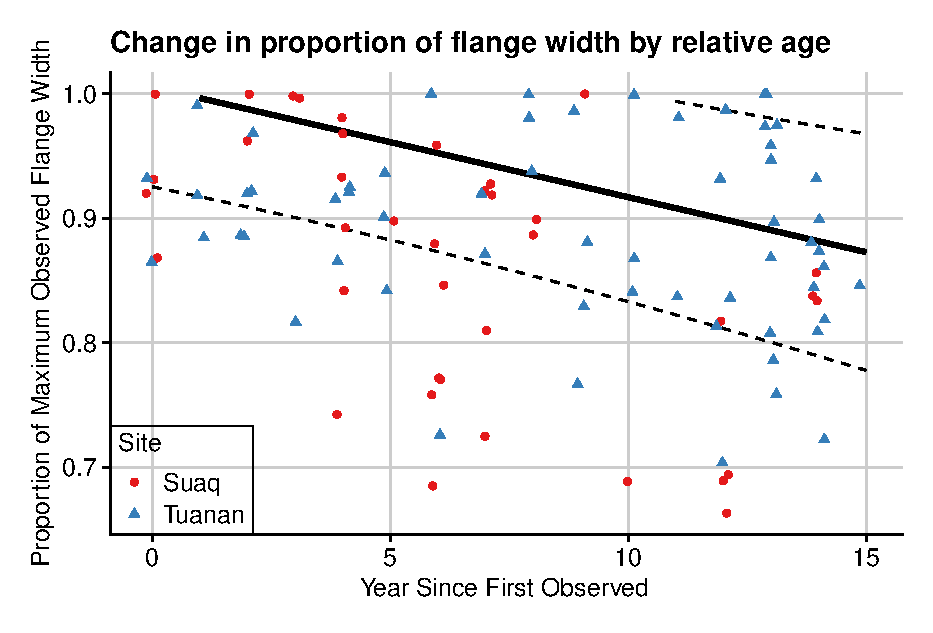
\includegraphics[width=0.8\linewidth]{Chapter3/Figs/flange_width.eps}
\caption{Examination of the impacts of ecological and social factors on flange width in orangutans across different sites. The plot presents the relationship between the number of years since the orangutan was first observed (YearSinceFirstSeenTab) and the proportion of maximum observed flange width (Prop\_eyeflange). Each point, differentiated by colour and shape according to the site, represents an observation from the data set. The lines with dashed boundaries show the predicted response and confidence intervals generated from the mixed model results.}
\label{fig:enter-label}
\end{figure}
\subsection{Impacts of relative flange size on long calls and mating success}

In the analysis of the effect of relative flange width on flanged male mating behaviour, five models were considered. Table 3.5. shows Models 9-11, based on count data.

Model 9 (Table 3.5.), focused on the number of long calls per follow day, found a statistically significant impact of relative flange width on the number of long calls produced per day (Estimate = -7.697, p-value = 0.034). Additionally, I found a significant impact of the total hours of rainfall per follow day on long call rates, albeit with a lower effect size (Estimate = 0.076, p-value = 0.025). However, no other explanatory variable was found to be significant.

 Model 10, which considered the number of pulses per long call per follow day, did not reveal significant impacts from any of the variables, except Total rain (hours) which showed a minor positive impact on the number of pulses per long call (Estimate = 0.011, p-value = 0.027).
 
Model 11, analysing the number of copulations per follow day, did not find any significant impacts between the proposed factors and the number of copulations per follow day. 

\begin{table}
    \centering
    \resizebox{\textwidth}{!}{%
    \begin{tabular}{l l r r r r}
    \hline 
    \multirow{2}{*}{\textit{Response}} &  \multirow{2}{*}{\textit{Fixed effects}} & \multirow{2}{*}{\textit{Estimate}} & \multirow{2}{*}{\textit{Std. Error}} & \multirow{2}{*}{\textit{z}} & \multirow{2}{*}{\textit{Pr(>|z|)}}\\ 
     & & & & & \\
    \hline
   \textbf{9. Number of long calls per follow day} & \textbf{Intercept} & \textbf{-2.632} & \textbf{3.278} & \textbf{-0.803} & \textbf{0.422} \\

   & \textbf{Prop\_eyeflange }& \textbf{-7.697} & \textbf{3.631} & \textbf{-2.120} & \textbf{0.034} \\
   
   \textit{Negaitve Binomial GLMM} & zFAI & 0.904 & 0.727 & 1.244 & 0.214\\
   
   \textit{Offset(ObsTime)} & Site (Tuanan) & 0.742 & 1.700 & 0.437 & 0.662\\
    
   N = 75, $\Delta$ AIC = 25.13 & \textbf{Long calls heard} & \textbf{0.231} & \textbf{0.118} & \textbf{1.965} & \textbf{0.049} \\
   
   & zAssocH & -0.091 & 0.275 & -0.331 & 0.741\\
   
   & \textbf{Total rain (hours)} & \textbf{0.076} & \textbf{0.034} & \textbf{2.237} & \textbf{0.025}\\
   
    \cline{2-6}
    
        & \textit{Random effects} & & & \textit{Variance} & \textit{Std. dev.}\\
        
    \cline{2-6} 
    
    & Name & & & 1.012e-09 & 3.181e-05 \\

    & Year:Name & & & 4.974 & 2.230 \\
    
    & Month:Year:Name & & & 5.625e-08 & 2.372e-04 \\
    
     \hline 

   \textbf{10. Number of pulses per long call} & \textbf{Intercept} & \textbf{2.477} & \textbf{0.934} & \textbf{2.654} & \textbf{0.008} \\

  & Prop\_eyeflange & 0.812 & 1.093 & 0.743 & 0.458 \\
   
   & zFAI & -0.055 & 0.204 & -0.271 & 0.787\\
   
    \textit{Negaitve Binomial GLMM} & Site (Tuanan) & -0.253 & 0.557 & -0.454 & 0.650\\
    
  & Long calls heard & 0.020 & 0.019 & 1.085 & 0.278 \\
   
 N = 29, $\Delta$ AIC = 2.034  & zAssocH & -0.052 & 0.061 & -0.851 & 0.395\\
   
   & \textbf{Total rain (hours)} & \textbf{0.011} & \textbf{0.005} & \textbf{2.212} & \textbf{0.027}\\
   
    \cline{2-6}
    
        & \textit{Random effects} & & & \textit{Variance} & \textit{Std. dev.}\\
        
    \cline{2-6} 
    
    & Name & & & 0.208 & 0.456 \\

     \hline 
   \textbf{11. Number of copulations per follow day} & \textbf{Intercept} & \textbf{-15.440} & \textbf{65.063} & \textbf{-0.237} & \textbf{0.812} \\

   & Prop\_eyeflange & -4.302 & 68.047 & -0.063 & 0.950 \\
   
   \textit{Poisson GLMM}, \textit{N = 23} & zFAI & -0.718 & 4.399 & -0.163 & 0.870\\
   
  \textit{Offset(FemAssocH)}  & Site (Tuanan) & -2.444 & 9.599 & -0.255 & 0.799\\
    
  N = 23, $\Delta$ AIC = 13.04  & Long calls made & 0.430 & 1.009 & 0.426 & 0.670 \\
      
    \cline{2-6}
    
        & \textit{Random effects} & & & \textit{Variance} & \textit{Std. dev.}\\
        
    \cline{2-6} 
    
 & Name & & & 8.494e-04 & 0.029 \\

    & Year:Name & & & 0.001 & 0.037 \\
    
    & Month:Year:Name & & & 76.10 & 8.723 \\
    
     \hline 
       \end{tabular}
}
    \caption{Results of the GLMMs exploring the impacts of relative flange width and ecological factors on number of long calls per follow day, number of pulses per long call and number of copulations.}
\end{table}
Table 3.6. shows Models 12-13, which are both based on continuous response variables. In Model 12, the response variable was the "Average duration of long call per follow day". None of the fixed effects demonstrated a significant impact on the duration of long call per follow day.  Model 13 aimed to understand the impact of these fixed effects on the number of hours in association with a female per follow day. Notably, zFAI demonstrated a significant impact, with an estimate of -1.30278 and a p-value of 0.048. However none of the other explantory variables showed a statistically significant impact.

\begin{table}
    \centering
    \resizebox{\textwidth}{!}{%
    \begin{tabular}{l l r r r r r}
    \hline 
    \multirow{2}{*}{\textit{Response}} &  \multirow{2}{*}{\textit{Fixed effects}} & \multirow{2}{*}{\textit{Estimate}} & \multirow{2}{*}{\textit{Std. Error}} & \multirow{2}{*}{\textit{df}} & \multirow{2}{*}{\textit{t}} & \multirow{2}{*}{\textit{Pr(>|t|)}}\\ 
     & & & & & & \\
    \hline
        \textbf{12. Average duration of long call per} & Intercept & 95.85126 & 60.62015 & 18 & 1.581 & 0.131 \\

  \textbf{follow day} & Prop\_eyeflange & -44.87252 & 70.46522 & 18 & -0.637 & 0.532 \\
   
   & zFAI & -1.78435 & 12.52036 & 18 & -0.143 & 0.888\\
   
    \textit{Gaussian GLMM}, \textit{N = 25} & Site (Tuanan) & -17.13861 & 25.83756 & 18 & -0.663 & 0.516\\
    
    & zAssocH & -0.14225 & 4.89118 & 18 & -0.029 & 0.977 \\
   
  N = 25, $\Delta$ AIC = 36.71 & LCH & 0.53515 & 1.37842 & 18 & 0.388 & 0.702\\
   
   & Total rain (hours) & 0.01575 & 0.37449 & 18 & 0.042 & 0.967\\
   
    \cline{2-7}
    
        & \textit{Random effects} & & & & \textit{Variance} & \textit{Std. dev.}\\
        
    \cline{2-7} 
    
    & Name & & & & 0 & 0 \\

    & Residual & & & & 541.7 & 23.28 \\
    
     \hline 

        \textbf{13. Number of hours in association} & Intercept & -1.40594 & 0.94322 & 74.30810 & -1.491 & 0.1403 \\

  \textbf{with a female per follow day} & Prop\_eyeflange & 1.52725 & 1.02205 & 86.91673 & 1.494 & 0.1387 \\
   
   & \textbf{zFAI} & \textbf{-0.19514} & \textbf{0.09292} & \textbf{96.48181} & \textbf{-2.100} & \textbf{0.0383}\\
   
    \textit{Guassian GLMM} & Site (Tuanan) & -0.15691 & 0.20012 & 25.63337 & -0.784 & 0.4402\\
    
\textit{Offset(ObsTime)}  & Long calls made & 0.04682 & 0.02471 & 94.76339 & 1.895 & 0.0611 \\
   
   
    \cline{2-7}
    
      N = 119, $\Delta$ AIC = 25.11  & \textit{Random effects} & & & & \textit{Variance} & \textit{Std. dev.}\\
        
    \cline{2-7} 
    
    & Name & & & & 0.01186 & 0.1089 \\

    & Year:Name & & & & 0.08261 & 0.2874 \\
    
    & Month:Year:Name & &&  &  0.00000 &  0.0000 \\

    & Residual & & & & 0.88910 & 0.9429 \\
    
     \hline 

    \end{tabular}
    }
    \caption{Results of the LMMs examining the impacts of relative flange width on average duration of long call and number of hours of female association per follow day. }
\end{table}



\section{Discussion}

The maintenance of SSCs can be metabolically costly for the individuals who produce them, however their ultimate impact on mating success depends on the mating system, dominance hierarchy and life history of the species \citep{Kappeler.2004}. 

\subsection{Impact of life history and ecological factors on flange size}
Our model which examined the hypothesised causes of flange reduction across all sites indicated that age was the best linear predictor of reduction in flange width (although this was not found to be significant in the Tuanan-only models, or on relative flange area). This is particularly notable as it suggests that the cause is likely not accumulated injuries and scar tissue on the flange, as these injuries can occur all over the flange rather than localised at the eye level. As these impacts were only seen in one model with a limited sample size, it is important not to overstate their significance, however they may be indicative of age related degeneration in the flange. Older individuals experience senescence, which may have several impacts on SSC maintenance. I suggest four non-mutually exclusive mechanisms for degeneration in flange size after initial development.

The first is age-linked reduction in testes volume, which in turn has an impact on circulating testosterone levels. In humans, males over the age of 60 experience a reduction in testes size of approximately 37\%, and mean serum testosterone levels start decreasing from the age of 50 \citep{Stearns.1974}. Across wild and captive studies, flanged males have significantly higher androgen levels than unflanged males, and individuals undergoing bimaturism have higher levels still indicating their importance to the development and maintenance of these characteristics \citep{Marty.2015rzq, Prasetyo.2021}. Hence an age-linked reduction in testosterone due to age may impact the maintenance of these SSCs. 

A second possible cause of a reduction in flange width with old age is sarcopenia, the deterioration of muscle tissue in elderly mammals. This progressive and generalised skeletal muscle disorder involves the accelerated loss of muscle mass and function \citep{Evans.1993}. In the case of the orangutan flange, which houses slips of several of the facial muscles \citep{Straus.1942}, such age-related muscle wasting could be particularly impactful. The loss of these muscle fibres might directly translate to a decrease in the structural support required for maintaining flange size, thereby leading to a decrease in the mass and volume of the flanges.

A third potential mechanism behind the age-related reduction in flange size may be tied to reduced vascularity associated with aging. The process of aging is linked to the diminished vascular supply of tissues, thereby limiting the amount of oxygen and nutrients delivered to these tissues, and subsequently impeding their repair and regeneration capabilities \citep{Prisby.2007}. Dissections of the orangutan flange, the skin and the underlying fatty pad appear to be quite vascular \citep{Straus.1942}. These regions are abundant with blood vessels, with some areas suggestive of erectile tissue due to the density of vasculature. Given this, the flanges might be particularly vulnerable to the effects of reduced vascularity that come with aging. The reduction in blood supply could deprive the fibrous and adipose tissues, which make up the bulk of the flange, of the necessary resources for maintenance and repair.
In the face of diminished vascularity, the fibrous framework consisting of collagenous septa, along with the lobules of fat and striated muscle fibres found in the flange \citep{Straus.1942, Winkler.1989}, might experience reduced nutritional and oxygen supply. This could potentially lead to a decrease in the integrity and mass of these components, subsequently contributing to a reduction in flange size. Hence, this relationship between reduced vascularity and the age-related decrease in flange size may serve as a compelling avenue for future research.

Finally, the structural integrity of flanges, which are largely composed of loose connective tissue whose framework consists of collagenous septa continuous with the fibres of the corium, might be impacted by age-related collagen deterioration \citep{Straus.1942}. As aging progresses, there is a decline in collagen synthesis, coupled with a slowing of the tissue remodelling process. This could lead to a decreased structural integrity of the collagenous framework of the flanges, rendering them less robust and potentially smaller. The accumulation of damage, as a result of less efficient tissue repair and replacement, could further contribute to the degradation of fibrous tissues in the flanges \citep{Cox.2011, Haus.2007}. As previously mentioned, these hypotheses are not mutually exclusive and these factors may act in synergy.

\subsection{Impact of FAI on flange morphology}

Contrary to my predictions, there was no significant impact of fruit availability on flange size. While the flange structure in orangutans does contain large lobules of fat, this adipose tissue might not be as responsive to changes in nutritional availability as those in other parts of the body. 

It is possible that once flanges have developed, they may not be subject to the same plasticity seen in other phenotypic traits. The flanges, consisting of collagenous septa, striated muscle fibres, and a dense network of blood vessels within a framework of adipose tissue \citep{Straus.1942, Kinglsey.1988} could be resistant to fluctuations in size due to environmental conditions. The high energetic cost associated with flange formation might make it metabolically impractical for the body to adjust these structures in response to varying fruit availability. In fact, this pattern aligns with what has been observed in other primates, such as gorillas, where the size of secondary sexual characteristics like the sagittal crest, remain largely unchanged after full development, despite variations in food availability \citep{Caillaud.2008m5r}.

Second, changes in fruit availability may affect aspects of the flanges other than their width or overall size. For example, reduced availability of nutrients could potentially impact the vascular integrity of the flanges or the health of the dermal papillae. The impact might be seen in visual changes, such as the reported deflated appearance associated with the "past-prime" condition, which could influence the male's attractiveness or social status without altering the overall width of the flanges. Further investigation is required to explore these possibilities and to gain a better understanding of how ecological variables such as fruit availability may impact the physiological characteristics of orangutan flanges using qualitative methodology, or dissection of flange specimens from a range of adults. Notably, a reduction in the volume of the flange that does not impact the area or width would not have been detected by my analyses, however detecting this change in future studies would likely prove difficult, as it would require detailed measurements of the flange in an environment where nutritional intake could be controlled in an manner consistent with animal welfare.

\subsection{Impact of observed antagonistic interactions}
Despite initial conjectures, my analyses focused on the Tuanan field station have found no observed relationship between relative flange size and the frequency or severity of antagonistic interactions. It was previously hypothesised that, due to repeated activation of the vertebrate stress response increasing allostatic loads, flange deformation might be linked to such antagonistic interactions. Across primate species, stress induced by these interactions is well documented to increase blood glucocorticoid concentrations via the activation of the hypothalamus–pituitary–adrenal axis \citep{Maestripieri.2011, Setchell.2016, Edes.2017}.

For example, in mandrills, chronic activation of the vertebrate stress response leads to persistently elevated blood glucocorticoid levels, negatively impacting individual outcomes, including reduced resistance to disease and compromised reproductive success \citep{Setchell.2010}. However, the impacts of stress are modulated by factors such as the individual's dominance ranking and the stability of the dominance hierarchy within the population. The Tuanan field station is characterised by an unstable dominance hierarchy, which is influenced by a high ratio of flanged to unflanged males and significant fluctuations in fruit production. Consequently, I had predicted that the dominant flanged males would experience the greatest social stress during antagonistic interactions \citep{Sapolsky.2005gvn}.

However, a key limitation of this study was the uniform scoring assigned to all antagonistic interactions, regardless of their severity, ranging from immediate withdrawal from the conflict to lethal aggression \citep{Knott.2008, Setia.2008}. Frequently witnessed consequences of these conflicts are mutilations, including loss of digits or bites that remove parts of the upper lip. If these injuries could be reliably dated to specific time frames, they could yield valuable insights for future research into the relationship between social stressors and physical alterations in orangutans. Nonetheless, the current methodology may have obscured potential impacts of the severity of antagonistic interactions on flange morphology, which presents an area for refinement in future studies.

\subsection{Impacts of flange deformation on long call behaviour}

Contrary to my predictions, individuals with a relatively less wide flange produced long calls more often than when their flange was at its fullest extent. Additionally, the total amount of rain hours in the day appears to increase the number of long calls produced, rather than decreasing it - contrary to the findings of previous studies \citep{Spillmann.2016}

One potential explanation for less wide flanged males producing more long calls might lie in their need for enhanced social communication. Orangutans whose flanges are relatively reduced may be lower in the local dominance hierarchy. These individuals might employ long calls more frequently as a strategic tool to communicate their presence, assert their territory, or possibly attract potential mates without engaging in direct physical confrontations, which they are less likely to win due to their less intimidating physicality. These results may also support the hypothesis from \citet{Mitani.1985}, that the flange also functions as a way of focusing the long call in a specific direction. If this hypothesis is correct, then individuals with relatively diminished flange size may need to produce long calls more often to counter the impacts of this condition.

Regarding the increase in the number of long calls with more rain hours, this might be tied to the acoustic properties of the rainforest environment during and after rainfall. It is possible that the ambient noise caused by rainfall masks the long calls, necessitating more frequent vocalisations and an increased number of pulses per vocalisation for effective signaling \citep{Spillmann.2016}. Additionally, during a downpour, the ambient noise levels in the rainforest drop significantly, which may be due in part to the physical impact on the vegetation. It can weigh down foliage, leading to fewer leaves rustling in the wind and therefore less background noise. However, gibbons vocalise less frequently after rainfall, and this quieter backdrop might enhance the audibility of orangutan long calls \citep{Clink.2020}. 

This study did not have access to the raw long call recordings and, as such, I was unable to examine any correlation between other aspects of the long call, including frequency or estimated amplitude with changes in flange width. As long call data sets increase with time, this may be an avenue of research in the future, however, currently long call recordings at Suaq Balimbing and Tuanan are not common enough, or collected over a long enough time to provide a rigorous analysis of longitudinal changes in long call frequency or amplitude.

\subsection{Impacts of flange deformation on female association patterns}

The absence of a direct relationship between flange width and the z-transformed hours of female association per follow day was contrary to my initial hypothesis. I had anticipated that a decrease in flange size would correspond with reduced association hours, under the assumption that physical characteristics such as flange size may be an important factor in female mate choice. However, the lack of evidence for this relationship in the model suggests that flange width might not be as influential a factor as I had initially proposed.

Interestingly, the results did indicate a significant relationship between z-transformed fruit availability and hours of female association, but in a direction opposite to what I had predicted. This counter-intuitive outcome implies that higher fruit availability corresponded with reduced hours of association with females.

One possible explanation for these observations could be that the females are using additional signals beyond their physical characteristics when associating with potential mates. For example, behavioural traits, such as aggressiveness or protectiveness, might be more important determinants of association patterns than physical traits like flange width. Alternatively, it is possible that the significance of flange size is obscured by other unmeasured factors that also affect female association patterns, including familiarity with the flanged male.

Regarding the unexpected inverse relationship between fruit availability and hours of female association, one possible hypothesis could be that when food is plentiful, females may be less dependent on males for resource access and hence spend less time in association. Alternatively, higher fruit availability could result in a more dispersed distribution of individuals within the population, thereby reducing the opportunity for association.

Future research will be needed to test these hypotheses and elucidate the complex interplay of factors affecting association patterns in the study population. Additionally, it would be interesting to investigate the potential role of other male physical and behavioural traits in female association patterns to gain a more nuanced understanding of mate selection processes in this species.

\subsection{Copulation rates}

Contrary to my initial expectations, the number of copulations per follow day did not decline with a decrease in the flange size. The absence of a significant association suggests that flange quality is not a determinate factor when a female is already in association with a male. This may suggest that there is a role of female choice before entering into an association with a male, likely when hearing a long call. However, in this study, I did not find an expected significant association between long calls made and total female association hours per follow day (Model 13). It is plausible that females are more inclined to prioritise other aspects of male behaviour, such as feeding tolerance or food sharing, when selecting mates. Consequently, these behavioural traits could be more strongly tied to reproductive success than flange size. Also to consider is the impact of forced copulations, as this study did not have sufficient data between proceptive and forced copulations this may mask the role of female choice when in association, which led to no detectable significant relationship. 

Similarly, the lack of a significant relationship between relative fruit availability (zFAI) and the number of copulations suggests that immediate ecological conditions, such as food availability, may not directly influence mating behaviours, despite previous studies indicating that they increase association rates \citep{Marshall.2008}. This points towards the possibility that mating activities in this species could be less susceptible to fluctuating resource availability than initially assumed.

However, it is crucial to interpret these findings with caution due to the relatively small sample size of this study. The low number of observations could limit the robustness of the findings and potentially mask existing relationships. A wider comparison between sites in future studies could provide a more reliable analysis of the interaction between relative flange size, mating behaviours, and ecological conditions.

\subsection{Questions not addressed}

One limitation of this study was the inability to examine the impacts of antagonistic social stress at Suaq Balimbing. Face-to-face antagonistic interactions between flanged males have never been observed at Suaq Balimbing, despite having the highest density of wild orangutans in the world. However, orangutans do utilise long calls as a form of confrontational assessment, and this has been used in some studies to estimate dominance, but due to the complexities of this analysis this was beyond the scope of this study \citep{Spillmann.2016}

Another unknown from this research is the correlation between the ecological, social and individual factors and the underlying hormonal processes that drive SSC development and maintenance. While hormonal impacts on flange development have been examined in captivity, the difficulties in obtaining and processing wild hormone samples have made a comprehensive study of the maintenance of these SSCs impractical at this stage.

Due to the suggested relationship between age and relative flange width, and in light of the limited sample size, further studies should seek to examine the relationship between age and mating behaviours in orangutans to examine correlations between age and deterioration of other SSCs (e.g. long call composition and duration) (see Chapter 4).

Finally, in this analysis, individual measures were pooled to assess overall patterns and trends. However, a more granular analysis within-subject vs. between-subjects could offer different insights \citep{Siracusa.2022}. This approach may be able to discern individual trajectories and pinpoint variations that may be unique to specific subjects. Although time constraints prevented the incorporation of this approach into the present study, it represents a promising avenue for future investigations. 

\nomenclature[z-SSC]{SSC}{Secondary Sexual Characteristic}
\nomenclature[z-LM]{LM}{Landmark}
\nomenclature[z-FAI]{FAI}{Fruit Availability Index}

%!TEX root = ../thesis.tex
%*******************************************************************************
%****************************** Fourth Chapter **********************************
%*******************************************************************************
\chapter{Age-Related Behavioural Shifts in Flanged Male Orangutans: Insights from Female Association Behaviour and Long Call Patterns}

Primates exhibit a wide range of age-related shifts in social and mating behaviour. Currently, age-related behavioural changes over the lifetime of male orangutans focus primarily on the shifts between the unflanged and flanged morph, and behavioural shifts in ageing flanged male orangutans remain under-researched. Building on previous findings linking age to flange deformation, this study sought to further examine the behavioural changes associated with ageing in these primates, particularly focusing on female association behaviour and long call patterns. This study examined six males from the date of their first long call observed to investigate changes in female associative behaviour and long call composition over time. My results indicate that older flanged males tend to have fewer hours of association with females and produce shorter long calls with fewer pulses. These behavioural trends in older flanged males align with observations in other ageing great apes which show an increase in solitude with age. However, the underlying reasons for this change, whether it is reduced attractiveness or a self-imposed choice, remain undetermined. Preliminary data also imply that younger flanged males might exhibit varied responses to certain long call triggers, potentially indicating an effort to establish territorial dominance. However, this behaviour may also be driven by increasing energetic costs for producing lengthy long calls in older males. This research offers initial insights into the potential reclusiveness of older flanged males and emphasises the importance of factoring in the approximate transition date from unflanged to flanged in future studies on long call behaviours.
   
\section{Introduction}

\subsection{Effects of ageing in primates}

The ageing process in primates is characterised by a number of physiological and physical changes that can have significant impacts on an individual's overall health and reproductive success \citep{Holloszy.2000}. Older individuals experience a gradual decrease in muscle mass and bone density, as these conditions limit mobility and strength they ultimately impact dominance, mating success and survival \citep{Lowenstine.2016, Almeling.2017}.  Decreases in bone density have been observed in ageing captive rhesus macaques, with a gradual decrease in bone density observed in both sexes \citep{Black.2001}. Furthermore, the skin undergoes alterations such as loss of elasticity, leading to wrinkles and slower wound healing \citep{Montagna.1972, Thomas.2001}. Visible changes related to age, such as alterations in skin condition or hair colour, can differ between sexes in their perceptibility and social implications, potentially influencing mate selection and rivalry. For example, \citet{Jolly.2009} found that adult ring-tailed lemur (\textit{Lemur catta}) coat condition deteriorated as the breeding season progressed and these effects were exaggerated in older individuals. 

In addition to these physical alterations, ageing is interlinked with changes in hormonal composition. For example, there is often a reduction in the production of growth hormones, contributing to the observed decreases in muscle mass and bone density \citep{Fischer.2011}. For example, female rhesus macaques show decreased levels of growth hormone (GH) compared to younger individuals \citep{Woller.2002}. Male primates exhibit a gradual decline in testosterone levels that is linked to a decrease in testes volume \citep{HANDELSMAN.1985, Strum.1991}. In males, this decrease in circulating testosterone further impacts muscle mass, bone density, and sexual drive \citep{Zohdy.2014, Kenny.2000}. Age-related declines in testosterone can also affect mental faculties, for example, in humans a decrease in testosterone levels during ageing has been associated with a decrease in visuo-spatial reasoning in men, and supplementation with testosterone increased performance levels \citep{Martin.2007}. Ageing can also alter the production and regulation of cortisol, affecting an individual's stress response, immunity, and metabolic processes \citep{Goncharova.2002}.  Ageing also presents specific challenges to fertility. Although male primates continue to produce sperm throughout their lives, sperm quality and quantity declines with old age, reducing fertility \citep{Sitzmann.2008}. However, female primates can undergo a cessation of ovulation defined as menopause \citep{Walker.2008}. The timing of this event in the life of individuals vary according to species, with some species such as macaques (\textit{Macaca spp.}) and humans undergoing menopause during mid-life, while other species experience much later, such as chimpanzees who appear to experience at the end of their life \citep{Herndon.2012}.  

In addition to these physical impacts, ageing appears to have significant impacts on sociality in primates. As individuals grow older, they can experience a decrease in the size of their social network and the amount of time spent in association with others \citep{Almeling.2017, González.2023}. In female rhesus macaques, older individuals selectively decrease the size of their social network without reducing the amount of time spent socialising, focusing on previous partners and kin \citep{Siracusa.2022}. Similarly, in Barbary macaques (\textit{Macaca sylvanus}), older females engaged in fewer social interactions, spent less time grooming when they did engage in interactions and maintained a smaller social network \citep{Almeling.2016}. However, this trend is not universal, and there are primates that do not show such decrease when ageing. For example, no notable change in social network size has been observed in male bonnet macaques (\textit{Macaca radiata}) \citep{Silk.1994}. Notably however, the trend towards a shrinking social circle shows sex-specific biases, whereby the socially dominant sex appears to be more likely to increase social interaction during ageing compared to the less dominant sex \citep{Corr.2003,Machanda.2020}. It is important to note that many of these studies focus exclusively on females, in part because males experience a higher mortality rate than females and because many studies have been conducted on female-philopatric species \citep{Machanda.2020}.
However, there are some wider differences between humans and most other primates, ageing humans show a notable positivity bias in their social interactions, while the more common trend in primates is a negativity bias. For example, male bonnet macaques show a decrease in the number of groomings initiated with age, while maintaining similar aggression rates to younger males \citep{Silk.1994}. Psychological studies on humans have found that they exhibit a selective memory bias towards positive events and emotions and prioritise engagements that affirm positive interactions as they age \citep{Carstensen.1999}. Interestingly, parallel findings are observed in one of our closest relatives, chimpanzees. Like humans, ageing chimpanzees appear to exhibit preferences for affiliative interactions, especially with well-acquainted conspecifics, and show a decrease in antagonistic encounters \citep{Rosati.2020}.  These trends are often attributed in part to inherently flexible social systems. This dynamism might enable older individuals to exert greater control over their social environment, associating more often with preferred companions and avoiding potential conflicts \citep{Aureli.2008}. Studies on humans have linked this shift towards positivity in social interactions to our ability to perceive our own limited time and re-organise our lives to prioritise emotional wellbeing over long-term goals, which is known as Socioemotional Selectivity Theory (SST) \citep{Carstensen.1999}. Although this trend is correlative with age, it is primarily driven by our perception of the remaining time and, therefore, is also affected by serious illness or significant life events \citep{Löckenhoff.2004}. However, given this requires significant levels of abstract reasoning about one's own mortality, it is unlikely to be the cause of the observed trend in chimpanzees. As such, alternative hypotheses have been suggested to explain these cross-species trends, noting that humans undergo an increased capacity to regulate emotional reactivity with age \citep{Rosati.2020,Grühn.2016}. However, a cross-species study on this alternative hypothesis has not yet been published.

In males these changes may correlate with impacts of ageing on social dominance, many primates show an inverted-U-shaped dominance curve, where older and younger adults are typically less dominant than "prime-aged" adults \citep{Packer.1979, Smuts.1989, Perlman.2016}. Younger adults are more likely to engage in risky behaviour, including challenging established leaders, while older individuals are generally more averse to risk \citep{Wilson.1985, Haux.2022}. This may be largely due to the increased resource-holding potential of prime-aged adults compared to older ones which combined with the increasing social isolation of elderly individuals and aversion to negative social interactions can lead to a sharp decrease in reproductive success when older. However, this framing removes the impact of female mate choice seen in polygynous or polgynandrous mating systems. For example, \citet{Foerg.1982} found that female black-and-white ruffed lemurs preferred older prime-aged males compared to younger ones, based on their ability to ignore challenges from sub-adult and younger prime males. However, in species with these mating systems,  senescence is experienced more severely by males compared to females, due to a combination of evolutionary and early life factors \citep{Graves.2007}. Species with high levels on intrasexual competition have a higher risk of mortality, which can lead to a reduction in the selection against deleterious mutations which can impact senescence \citep{Williams.1957}. 

\subsection{Sexual strategies and ageing in orangutans}

Orangutans are unique among the primate family in displaying irreversible bimaturism, with both the flanged and unflanged male morphs being able to sire offspring \citep{Knott.2008, Utami.2002km8}. As bimaturism can be arrested by social and psychoendoneurological factors, some unflanged males can sire children from as old as 40 without undergoing this transition \citep{Prasetyo.2021} . Given the dispersed polygynous mating system and female preference for flanged males, we see strong competition between males for access to mates and a significant role of female choice in this environment \citep{Harrison.2007ox}. 

Under these conditions, each morph has a different mating strategy to maximise their number of copulations given their secondary sexual characteristics. The larger of the two, the flanged male, possesses most notably a complex laryngeal sac and cheeks pads, and operate a "call and wait" strategy by emitting distinctive long calls and waiting for females to approach \citep{Utami.2002km8, Kunz.2023}. Interactions between flanged males are almost always antagonistic and can result in serious injury or death to the losing party \citep{Setia.2008}. However, given their semi-social lifestyle, flanged males also indirectly assess competition by use of characteristic long calls \citep{Spillmann.2016}. The call starts with a low rumble and builds up to a crescendo of roars and pulses before ending with a series of gurgles \citep{Spillmann.2010}. These long calls can be heard from up to 1.5km away, however they may only be individually identifiable within a range of 400m \citep{Spillmann.2016}. The role of the flange in this strategy remains unclear. Some suggest that the slightly concave shape of the flange aids the individual in locating the source of other long calls, while others believe it helps to focus the long call in a particular direction \citep{Galdikas.1983,Mitani.1985ak1m}. Current research has not found an association between long call rates and fruit availability, suggesting that they are not costly to make, however, the structure of each long call is context dependent and can be triggered by local cues \citep{Spillmann.2016}. Long calls can occur spontaneously, in response to another long call from a different individual and after pushing over a tree \citep{Delgado.2008}. Females seem able to discern the causes of specific long calls, and move a greater distance towards the source of spontaneously produced long calls, than cued long calls \citep{Spillmann.2016}.  

Females also respond to long calls differently, depending on their habitat. In Suaq Balimbing, female orangutans always move towards the long caller, regardless of their reproductive state, while in Tuanan females move towards long calls only if they do not have dependent offspring \citep{Dunkel.2013, Spillmann.2016}. However, these choices are also mediated by the dominance hierarchy of the local area, in sites with stable dominance hierarchies, females are more likely to be found in the presence of the dominant flanged males, and have longer associations with them compared to non-dominant males \citep{Setia.2008}. After approaching a male, females in association can experience attempts from males to force copulation. This degree of direct sexual coercion is unique among great apes, and given the rates of physical wounding during these encounters is very low, \citet{Knott.2009y9d} argues that these mating attempts are \textit{"direct coercion, and not an indirect means to influence or control future female sexual behavior, as seen in species such as chimpanzees and humans"}. Typically this is framed as an unflanged:flanged dichotomy, that due to female preference for flanged males, unflanged males resort to forced copulation; however, rates of forced copulation vary according to study site and dominance hierarchy \citep{Knott.2008, Knott.2009}. For example, in Suaq Balimbing, the ratio of unflanged males to flanged males is significantly higher, and flanged males employ forced matings significantly less than in Bornean field sites, suggesting that females may be moving towards males as a form of protection against forced matings \citep{Knott.2008}. 

\citet{Knott.2009y9d} also reported that a paper then in preparation found female proceptivity to mating attempts also vary according to the body condition of flanged males at Gunung Palung. Reportedly, males classified as "past-prime" based on their body condition and dimished flange size associated with females significantly less, and females were highly resistive to copulation attempts from them. Additionally, this same paper suggested that males in this condition produced long calls at a lower rate than "prime" males \citep{Knott.2009y9d}. These reported changes in calling behaviour are reinforced by own findings indicating a shift in long call behaviour with diminishing flange width (Chapter 3). Chapter 3 found that the main correlative cause of this condition is increasing age, which is expected to have significant impacts on health particularly in sexually dimorphic species \citep{Beirne.2015}. These age-related changes may then reduce their competitiveness in contests between other flanged males, and reduce the quality of their secondary sexual signals.

Given that long calls have unique patterns that can be used for individual identification, and that females seem to be able to discern the causes behind specific calls, it is possible that the composition or structure of the call is affected by the health of the individual that produces it \citep{Spillmann.2017}. Assuming long calls are not energetically costly, as hypothesised previously, the long call rate is unlikely to be unbiased indicators of fitness, however, we may see impacts on the duration or underlying structure \citep{Zahavi.1975}. It is also possible that the structure of the call remains unchanged, but the female response to long calls is affected and moves a shorter distance towards the call before stopping \citep{Spillmann.2010}.

If these calls are diagnostic of individual body condition, we may also see a shift in mating strategy from ageing flanged males from a "call and wait" strategy to a "silent searching" strategy to avoid antagonistic interactions from flanged males likely to win antagonistic interactions. However, this strategy requires a significant amount of time ranging per day, which flanged males typically do not do and given their increased body size such a shift would require a significant increase in energy intake per day \citep{Prasetyo.2021}. However, if these calls do not contain enough information to diagnose individual fitness, then interaction rates will be similar, but the interactions themselves will be impacted once association has begun. 

In this study, I aim to examine the impacts of old age on orangutan mating and long call behaviour using long-term behavioural data sets. I hypothesise that the previously observed relationship between relative orangutan flange width and age (Chapter 3) will have secondary impacts on mating, and long call behaviours will impact flanged male orangutan mating success as they grow older. I also hypothesise that these impacts will be exaggerated by the self-imposed reduction in sociality experienced by many great apes.

Given the impacts of ageing on sociality and mating success across primates and great apes, and given the high density of flanged males and subsequent unstable dominance hierarchy at the study site; I predict:

\begin{enumerate}
    \item   Older flanged males will enter into fewer female associations per day.

    \item When older flanged males do enter into associations with females, they will be shorter than associations between younger flanged males and females.

    \item Older flanged males will be found in association with fertile females less often than younger flanged males.

    \item Older flanged males will produce long calls more often, but with fewer pulses and for a shorter period of time compared to younger flanged males.
\end{enumerate}


\section{Methods}
\subsection{Study site}
Data was collected at Tuanan Orangutan Research Project (2°09'S, 114°26'E) which is located in the Mawas Reserve in Central Kalimantan, Borneo. Orangutans have been followed daily since 2003 and has one of the highest densities of orangutans in Borneo containing approximately 4.5 individuals/km$^{2}$ \citep{Husson.2008}. The site contains a higher number of flanged males compared to unflanged males with approximately 60\% of male focal follows being conducted on flanged males and has an unstable dominance hierarchy between flanged males \citep{Dunkel.2013}. The study site is located within a low-altitude peat-swamp forest, with a history of anthropogenic disturbance \citep{Gaveau.2014}.


\subsection{Behavioural data}
Behavioural data was collected during daily nest to nest behavioural follows using 2 minute instantaneous focal sampling using an established protocol \citep{OU_methods}. To control for variation in association behaviour over the day, and as orangutans are more likely to be located when in association with other party members, only full day focal follows were included in this analysis (\textit{i.e.} followed from nest to nest). Additionally, the number of observation hours per follow was added as an offset to relevant GLMMs. Individuals were only included if they had been observed in the study site in their unflanged morph, for two key reasons. Firstly, the absolute age of all flanged males at Tuanan is not known, age was encoded as either the number of years since they were first observed or, if they were observed in their unflanged state the number of years since they grew their flanges is known. As unflanged orangutans are significantly more social than flanged males and to avoid systematic biases, I chose to exclude all flanged males where their flanging date is unknown. I then coded the flanged date as the first date for which these individuals produced a long call. These totalled 3,256 of focal follow hours across 6 individuals, collected between 2009 and 2018. 

\begin{figure}
\centering
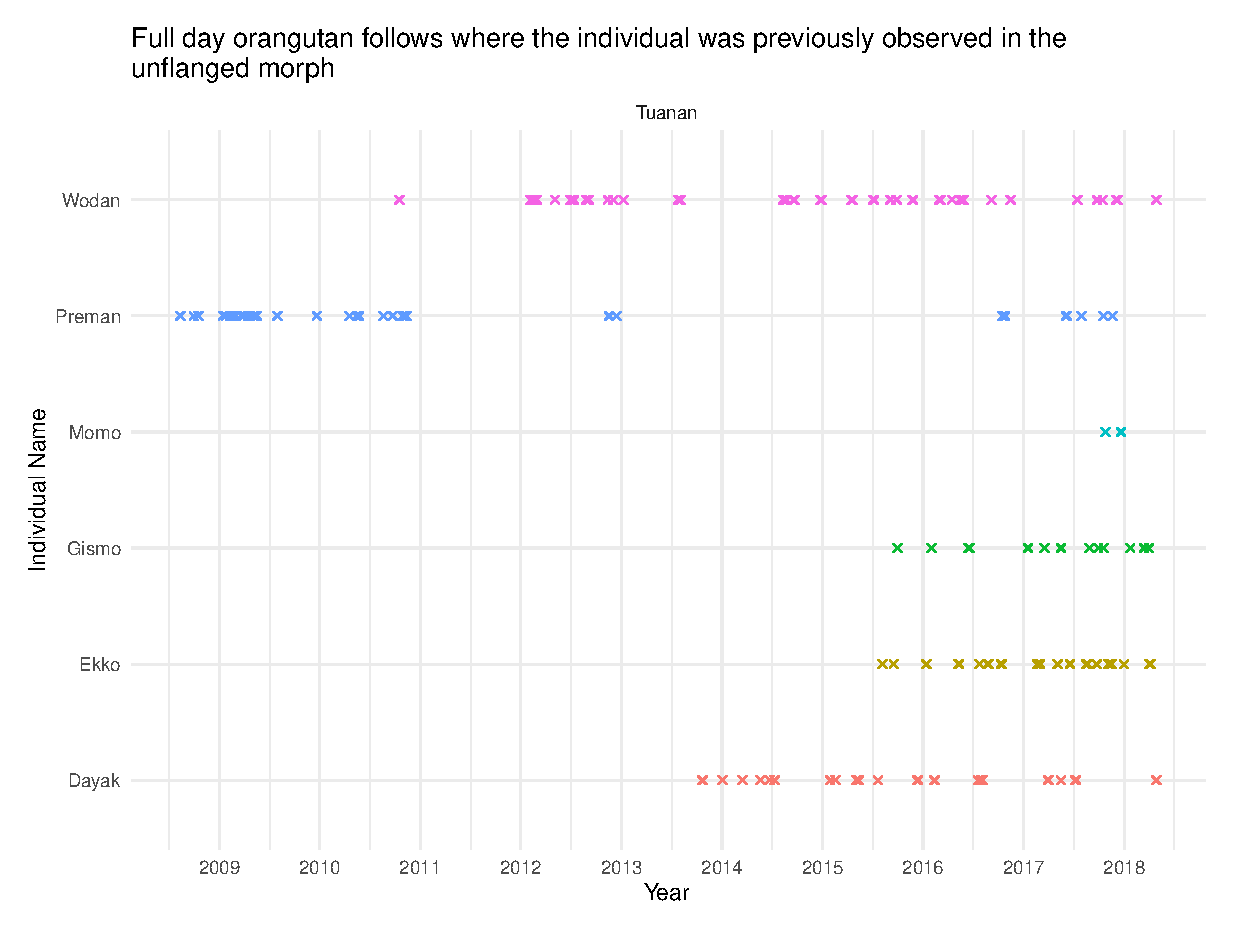
\includegraphics[width=1\linewidth]{Chapter4/Figs/obs_plot.eps}
\caption{Timeline (x-axis) illustrating days where a flanged male previously observed in their unflanged morph was followed for a full follow day at Tuanan Reserach Station. }
\label{fig:Obs_Tuanan_NN}
\end{figure}


\textbf{Association patterns}

Female association patterns were examined by estimating the duration of female association per focal follow day, and the number of females associated with per follow day.  Total female association time was measured as the total number of 2 minute intervals per follow where the focal flanged male was within 50m of a female. Female association time was additive if multiple females were present \textit{e.g.} if two females were present for one 2 minute bout, this would be measured as 4 minutes of female association. The number of females in association per focal follow day was examined using a Poission GLMM, and the total number of female association hours was examined using a Gaussian GLMM. In each model, FAI and relative age were added as fixed effects. As female association can be affected by the number of long calls (LCM) produced by an individual, this was added as a fixed effect for models concerning female association \citep{Spillmann.2010}. As females conceal ovulation and appear to selectively mate according to their fertility, the estimate of female fertility was based on the estimated dates of conception of females \citep{Knott.2009}. Females were coded as likely fertile from one year before estimated conception, or 3 months before the first swelling appears. Only one copulation was observed in our sample, so no copulation analysis has been conducted.

\textbf{Long call patterns}

Long call rates per follow-day and long call pulses per long call were modelled using Poisson GLMMs, and long call duration was modelled using a Gaussian GLMM. As long calls are context dependent and can be used as a form of confrontational assessment, the number of long calls made by other non-focal flanged males that were heard by the observers was included as a term in these analyses \citep{Spillmann.2016}. As long as call behaviour is affected by proximity to females, the number of hours spent within 50m of a female was used a fixed effect \citep{Spillmann.2010}. As association rates are impacted by fruit availability, an interactive effect between FAI and female association was added to our long call models; however, these were not found to be statistically significant, so were removed from our outputs. Additionally, rainfall can have a significant impact on primate calling behaviour; total daily rainfall was included as a term in all long call models (Chapter 3). Finally, relative age, fruit availability, and an interactive term between female association and fruit availability were added as fixed effects. 

\subsection{Ecological data}
Phenological data on fruit availability was taken monthly at both sites throughout the entire study period. The Fruit Availability Index (FAI) was calculated as the percentage of trees with fruits across all surveyed trees (approximately 1000) in the study site. 

\subsection{Analysis}

GLMM analysis was performed using the R version 4.3.0 using the \textit{glmmTMB} package to account for zero-inflated data common with behavioural data sets \citep{R.2018, Brooks.2017}. 

All Poisson GLMMs were tested for over‐dispersion by generating an over-dispersion statistic using the sum of the squared Pearson residuals. If data in a model with Poisson distribution revealed over‐dispersion, I conducted negative binomial GLMMs as an alternative. All Gaussian GLMMs were examined to confirm the normality of residuals and homoscedasticity to validate the model's fit. This was achieved via visual inspection of Q-Q plots and residual versus fitted value plots. All models included observation time (hours) as an offset variable to account for different day lengths. All models were created with the nested random intercept of (1|Name/Year/Month); however, in the instance of singularity errors, the random intercept was reduced to (1|ID). Each model was compared to a null model of $Response \sim 1 + (1|Name/Year/Month)$, with the change in AIC provided for each model in the table. The full null model outputs are provided in Appendix 2. 

All plots were produced using \textit{ggplot2} and \textit{ggeffects} was used to illustrate model effects \citep{Wickham.2011,Lüdecke.2018}. All statistical tests are two-tailed unless otherwise stated, and statistical analysis was performed in R version 4.3.0 \citep{R.2018}.  Factors that explain significant variation in the outcome variable with a p-value < 0.05 are indicated in bold.

\subsection{Ethical note}
Behavioural data collection was strictly observational and non-intrusive. There was no engagement between observers and the wild orangutans; a minimum distance of 10 metres was maintained to ensure the subjects' natural behaviour remained uninfluenced. The procedures for data gathering were in line with Indonesia's legal stipulations and received approvals from the Indonesian State Ministry for Research and Technology (RISTEK), the Directorate General of Natural Resources and Ecosystem Conservation - Ministry of Environment and Forestry of Indonesia (KSDAE-KLHK), the Ministry of Internal Affairs, Indonesia, the Nature Conservation Agency of Central Kalimantan (BKSDA), and the Balai Besar Taman Nasional Gunung Leuser (BBTNGL).

\section{Results}

\subsection{Impact of relative age on female association}

In order to investigate the relationship between age and female association dynamics, I used three linear mixed models. Models 1 and 2 used Poisson GLMMs to examine the impact of number of years since flanging on the number of females in association on a full follow day (Table 4.1.) For the response variable "Number of females in association" (Model 1), the model showed a strong significant intercept (Estimate = -12.487, p-value < 0.001). The years since flanging showed a negative, but non-significant trend (Estimate = -0.083, p-value = 0.431). FAI, or the Fruit Availability Index, had a very minor and non-significant effect (Estimate = -0.009, p-value = 0.912). The LCM effect was also found to be non-significant (Estimate = -0.054, p-value = 0.243). The variance associated with individual names, year-to-name, and month-year-to-name was 0.469, 7.630e-06, and 4.206e-07 respectively, showing that individual variation was the dominant source of random variability in this model.

Model 2 focused on the number of likely fertile females in association per full follow day. This also showed a significant intercept (Estimate = -11.583, p-value < 0.001). No significant effect was observed with the years since first seen (Estimate = -0.469, p-value = 0.063) on the number of likely fertile females in association. Furthermore, the impact of FAI was found to be significant and negative (Estimate = -0.328, p-value = 0.036). However, LCM appeared to be a non-significant factor in this model (Estimate = -0.080, p-value = 0.401). When examining the random effects, individual identity was the major contributor to variability (Variance = 4.328), as observed in Model 1.

\begin{table}
    \centering
    \resizebox{\textwidth}{!}{%
    \begin{tabular}{l l r r r r}
    \hline 
   \multirow{1}{*}{\textit{Response}} &  \multirow{1}{*}{\textit{Fixed effects}} & \multirow{1}{*}{\textit{Estimate}} & \multirow{1}{*}{\textit{Std. Error}} & \multirow{1}{*}{\textit{z}} & \multirow{1}{*}{\textit{Pr(>|z|)}}\\ 
\hline
\textbf{1. Number of females in association} & \textbf{Intercept} & \textbf{-12.487} & \textbf{0.671} & \textbf{-18.614} & \textbf{< 0.001} \\
  & Years Since Flanged & -0.083 & 0.105 & -0.787 & 0.431 \\
\textit{Poisson GLMM}, \textit{N = 188} & FAI & -0.009 & 0.082 & -0.111 & 0.912 \\
\textit{Offset(ObsTime)} & Long Calls Made & -0.054 & 0.047 & -1.166 & 0.243 \\
\cline{2-6}
$\Delta$ AIC = 84.715 & \textit{Random effects} & & & \textit{Variance} & \textit{Std. dev.}\\
\cline{2-6} 
& Name & & & 0.469 & 0.685 \\
& Year:Name & & & < 0.001 & 0.003 \\
& Month:Year:Name & & & < 0.001 & < 0.001 \\
\hline
 \textbf{2. Number of likely fertile females in association} & \textbf{Intercept} & \textbf{-11.583} & \textbf{1.882} & \textbf{-6.154} & \textbf{< 0.001} \\
      & Years Since Flanged & -0.469 & 0.252 & -1.862 & 0.063 \\
        \textit{Poisson GLMM}, \textit{N = 39} & \textbf{FAI} & \textbf{-0.330} & \textbf{0.157} & \textbf{-2.093} &\textbf{ 0.036} \\
        \textit{Offset(ObsTime)} & Long Calls Made & -0.080 & 0.096 & -0.841 & 0.401 \\
        \cline{2-6}
      $\Delta$ AIC = 2.892 & \textit{Random effects} & & & \textit{Variance} & \textit{Std. dev.} \\
        \cline{2-6} 
        & Name & & & 4.328 & 2.080 \\
        & Year:Name & & & < 0.001 & < 0.001 \\
        & Month:Year:Name & & & < 0.001 & < 0.001 \\
        \hline
    \end{tabular}
    }
    \caption{Results of the Poisson mixed-effects models examining the impacts of Years since flanged, long calls made and fruit availability on female association. The fixed effects used were number of years since flanged, Fruit Availability Index (FAI) and long calls made. This model included random effects for individual ID nested within Year and Month.
    Formula used was: \(ResponseVariable \sim YearSinceFlanged + FAI + LCM + (1 |Name/Year/Month)\) }
\end{table}
Model 3 (Table 4.2.) is a Gaussian GLMM mixed-effects model examining how the time spent in association with a female (per follow day) is influenced by various factors. Model 3 shows a significant negative relationship between the years since flanging and the hours in association with a female. Specifically, for every year increase since flanging, there was a decrease of approximately 0.4739 hours in association time (Fig. 4.2., Estimate = -0.474, p < 0.001). However, the impacts of the Fruit Availability Index (FAI) and number of long calls made per follow day were not statistically significant (Estimate = 0.040,  p = 0.749; Estimate = -0.141, p = 0.054). 
\begin{table}
    \centering
    \resizebox{\textwidth}{!}{%
\begin{tabular}{l l r r r r}
\hline 
\multirow{1}{*}{\textit{Response}} &  \multirow{1}{*}{\textit{Fixed effects}} & \multirow{1}{*}{\textit{Estimate}} & \multirow{1}{*}{\textit{Std. Error}} & \multirow{1}{*}{\textit{z}} & \multirow{1}{*}{\textit{Pr(>|z|)}}\\ 
\hline
\textbf{3. Hours in association with a female} & \textbf{Intercept} & \textbf{-7.761} & \textbf{1.176} & \textbf{-6.600} & \textbf{< 0.001} \\
\textbf{  per follow day} & \textbf{Years Since Flanged} & \textbf{-0.474} & \textbf{0.135} & \textbf{-3.504} & \textbf{< 0.001} \\
\textit{Offset(ObsTime)} & FAI & 0.040 & 0.123 & 0.320 & 0.749 \\
\textit{Gaussian GLMM}, \textit{N = 187} & Long Calls Made & -0.141 & 0.073 & -1.930 & 0.054 \\
\cline{2-6}
$\Delta$ AIC = 4156.204 & \textit{Random effects} & & & \textit{Variance} & \textit{Std. dev.}\\
\cline{2-6} 
& Name & & & 3.522 & 1.877 \\
& Residual & & & 9.874 & 3.142 \\
\hline 
\end{tabular}
    }
    \caption{Results of the Gaussian mixed-effects models examining the impacts of Years since flanged, long calls made and fruit availability on female association time per day. The fixed effects used were number of years since flanged, Fruit Availability Index (FAI) and long calls made. This model included random effects for individual ID nested within Year and Month.
    Formula used was: \(ResponseVariable \sim YearSinceFlanged + FAI + LCM + (1 |Name/Year/Month)\) }
\end{table}


\begin{figure}
\centering
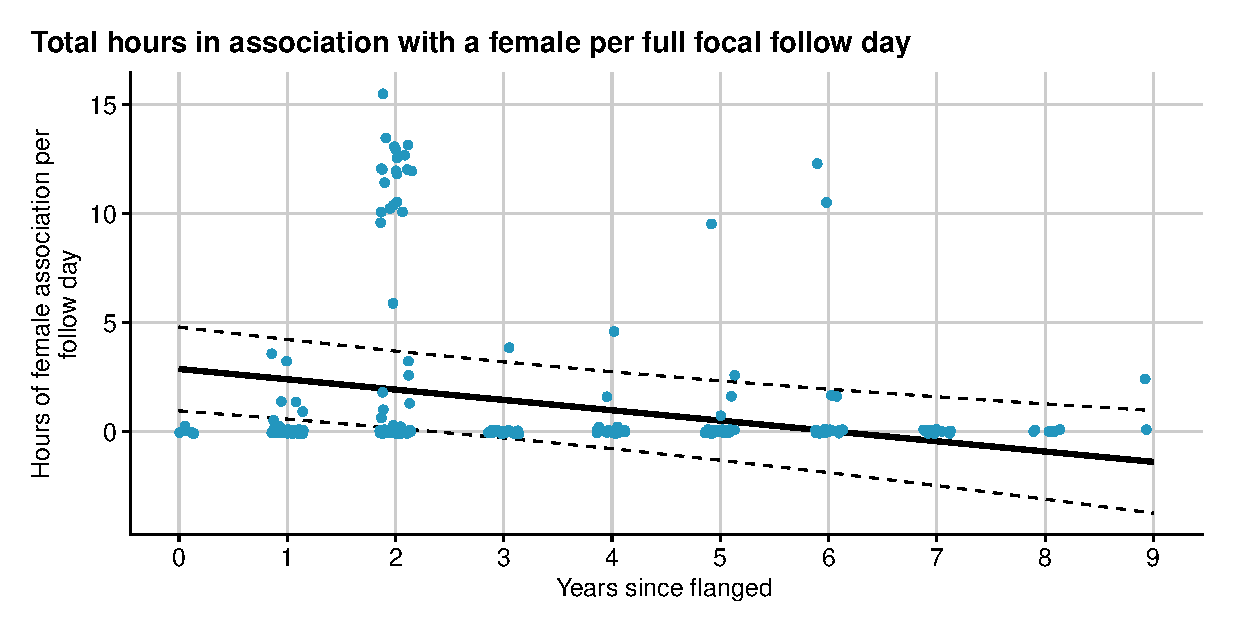
\includegraphics[width=1\linewidth]{Chapter4/Figs/FemAssocPlot.eps}
\caption{Examination of the impacts of ecological and social factors on the total hours of female association per full focal follow day. The plot presents the relationship between the number of years since the orangutan was first produced a long call and the total number of hours per follow day they spent within 50m of a female. The lines with dashed boundaries show the predicted response and confidence intervals generated from the mixed model results.}
\label{fig:Female Association Dynamics with Flanged Males as a function of Age in Tuanan Field Station}
\end{figure}

\subsection{Impact of relative age on long call behaviour and composition}

To examine the impacts of age since flanging, I used three more linear mixed effects models. I conducted two Poisson GLMMs to investigate the number of long calls per follow day and the average number of pulses per long call (Table 4.3).

Model 4 (Table 4.3) focused on the number of long calls per follow day. FAI had a positive impact on the number of long calls, being marginally significant (Estimate = 0.079, p-value = 0.046). However, all other fixed effects, did not have a signficant effect on the number of long calls produced per day (Years since flanged: Estimate = -0.009, p-value = 0.857; hours in female association: Estimate = -0.176, p-value = 0.081; total hours of rain: Estimate = -0.003, p-value = 0.439; number of long calls heard: Estimate = 0.014, p-value = 0.280).

Model 5 (Table 4.3) examined the average number of pulses per long call (including long call duration as an offset term). I found a strong negative relationship between Year since flanged and the average number of pulses per long call, which was statistically significant (Fig. 4.3., Estimate = -0.0821, p-value < 0.001). The number of long calls heard (LCH) also showed a negative association with the number of pulses per produced long call and was also statistically significant (Estimate = -0.01986, p-value = 0.02488).
As seen in Model 4, hours of female association, FAI and total rain were not significant predictors, with p-values of 0.110 and 0.958, respectively.

\begin{table}
    \centering
    \resizebox{\textwidth}{!}{%
\begin{tabular}{l l r r r r}
\hline 
\multirow{1}{*}{\textit{Response}} &  \multirow{1}{*}{\textit{Fixed effects}} & \multirow{1}{*}{\textit{Estimate}} & \multirow{1}{*}{\textit{Std. Error}} & \multirow{1}{*}{\textit{z}} & \multirow{1}{*}{\textit{Pr(>|z|)}}\\ 
\hline
\textbf{4. Number of long calls per follow day} & \textbf{Intercept} & \textbf{-1.488} & \textbf{0.334} & \textbf{-4.458} & \textbf{< 0.001} \\
& Years Since Flanged & -0.009 & 0.048 & -0.180 & 0.857 \\
\textit{Poisson GLMM}, \textit{N = 110} & \textbf{FAI} & \textbf{0.079} & \textbf{0.039} & \textbf{2.005} & \textbf{0.046} \\
\textit{Offset(ObsTime)} & FemAssocH & -0.176 & 0.101 & -1.743 & 0.081 \\
$\Delta$ AIC = 328.158  & Total Rainfall (h) & -0.003 & 0.004 & -0.773 & 0.439 \\
& Long Calls Heard & 0.014 & 0.013 & 1.081 & 0.280 \\
\cline{2-6}
& \textit{Random effects} & & & \textit{Variance} & \textit{Std. dev.}\\
\cline{2-6} 
& Name & & & 0.179 & 0.423 \\
& Month:Name & & & < 0.001 & < 0.001 \\
& Year:Month:Name & & & 0.205 & 0.453 \\
\hline 
\textbf{5. Average number of pulses per long call} & \textbf{Intercept} & \textbf{0.767} & \textbf{0.136} & \textbf{5.636} & \textbf{< 0.001} \\
 & \textbf{Years Since Flanged} & \textbf{-0.082} & \textbf{0.023} & \textbf{-3.521} & \textbf{< 0.001} \\
\textit{Poisson GLMM}, \textit{N = 102} & FAI & 0.008 & 0.020 & 0.404 & 0.686 \\
& FemAssocH & -0.103 & 0.064 & -1.598 & 0.110 \\
$\Delta$ AIC = 459.604 & Total Rainfall (h) & -0.001 & 0.002 & -0.052 & 0.959 \\
& \textbf{Long Calls Heard} & \textbf{-0.020} & \textbf{0.009} & \textbf{-2.243} & \textbf{0.025} \\
\cline{2-6}
& \textit{Random effects} & & & \textit{Variance} & \textit{Std. dev.}\\
\cline{2-6} 
& Name & & & 0.014 & 0.120 \\
& Month:Name & & & < 0.001 & < 0.001 \\
& Year:Month:Name & & & 0.048 & 0.219 \\
\hline 
\end{tabular}

}
    \caption{Results of the Poisson mixed-effects models examining the impacts of years since flanged, Fruit Availability Index, total hours of rainfall, female association (hours), and long calls heard on the number of long calls, and number of long call pulses per full focal follow day. These models include random effects for individual ID nested within Year and Month.
    Formula used was: \(Response \sim YearsSinceFlanged + FAI + FemAssocH + TotalRainfall.h + LCH + (1 |Name/Year/Month)\) }
\end{table}
Finally, Model 6 (Table 4.4.) examined the relationships of the fixed effect on average long call duration. This model found a significant negative relationship between the number of years since flanging and average long call duration, with individuals who have been flanged longer producing significantly shorter long calls (Fig. 4.3., Estimate = -2.6961, p-value = 0.011). However, all other fixed effects did not have a statistically significant impact on average long call duration (FAI: Estimate = 0.2879, p-value = 0.7192; FemAssocH: Estimate = -0.9427, p-value = 0.7721; total hours of rainfall: Estimate = -0.1591, p-value = 0.2031; long calls heard: Estimate = -0.3899, p-value = 0.4146).
\begin{table}
    \centering
    \resizebox{\textwidth}{!}{%
\begin{tabular}{l l r r r r}
\hline 
\multirow{1}{*}{\textit{Response}} &  \multirow{1}{*}{\textit{Fixed effects}} & \multirow{1}{*}{\textit{Estimate}} & \multirow{1}{*}{\textit{Std. Error}} & \multirow{1}{*}{\textit{z}} & \multirow{1}{*}{\textit{Pr(>|z|)}}\\ 
\hline
\textbf{6. Average long call duration per follow day} & \textbf{Intercept} & \textbf{49.584} & \textbf{5.796} & \textbf{8.555} & \textbf{< 0.001} \\
& \textbf{Years Since Flanged} & \textbf{-2.696} & \textbf{1.061} & \textbf{-2.541} & \textbf{0.011} \\
\textit{Gaussian GLMM}, \textit{N = 64} & FAI & 0.288 & 0.801 & 0.360 & 0.719 \\
& FemAssocH & -0.943 & 3.254 & -0.290 & 0.772 \\
$\Delta$ AIC = 455.311  & Total Rainfall (h) & -0.159 & 0.125 & -1.273 & 0.203 \\
& Long Calls Heard & -0.390 & 0.478 & -0.816 & 0.415 \\
\cline{2-6}
& \textit{Random effects} & & & \textit{Variance} & \textit{Std. dev.}\\
\cline{2-6} 
& Name & & & 20.5 & 4.528 \\
& Residual & & & 143.8 & 11.992 \\
\hline 
\end{tabular}
}
    \caption{Results of the Gaussian mixed-effects model examining the impacts of years since flanged, Fruit Availability Index, total hours of rainfall, females association (hours) and long calls heard on the average duration of long calls made per full focal follow day. This model includes a random effect for individual ID.
    Formula used was: \(Response \sim YearsSinceFlanged + FAI + FemAssocH + TotalRainfall.h + LCH + (1 |Name/Year/Month)\) }
\end{table}






\begin{figure}
\centering
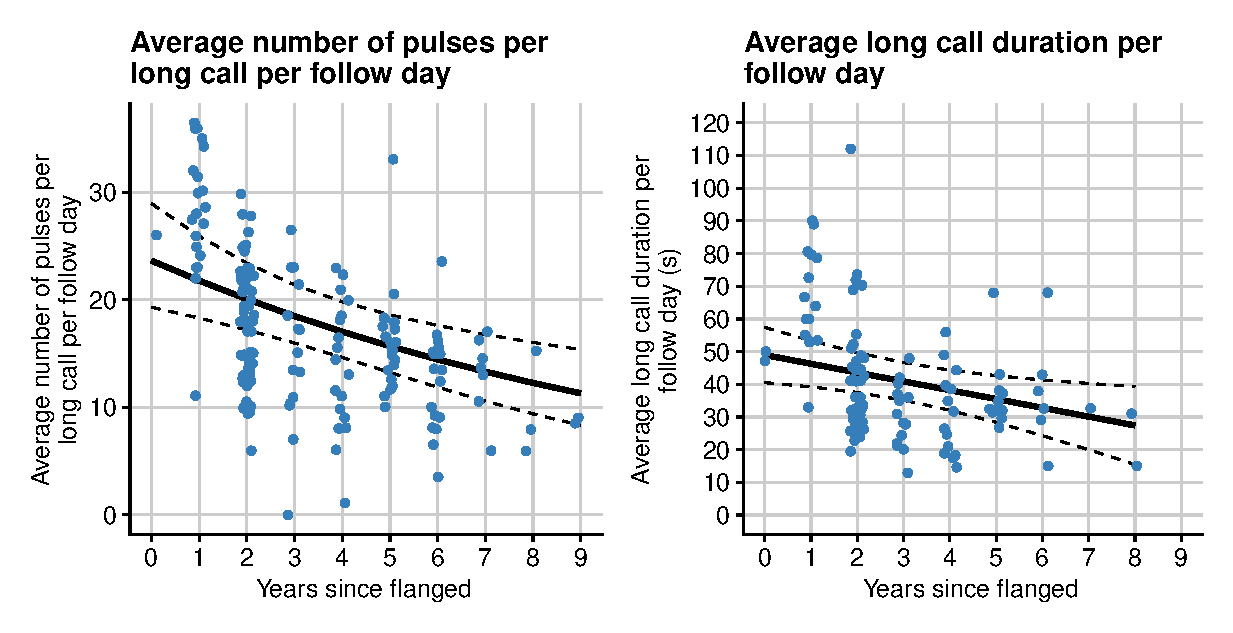
\includegraphics[width=1\linewidth]{Chapter4/Figs/combined_plot.eps}
\caption{Impacts of ageing on long call composition and duration. The left plot shows how the average number of pulses changes according to relative age since flanging. The right plot shows how average long call duration per day is impacted by relative age since flanging.}
\label{fig:Flanged_male_association_between_Suaq_and_Tuanan}
\end{figure}



\section{Discussion}

The combination of semi-social social structure, unflanged ranging behaviour, and bimature male physiology makes examining the impact of age on sociality in wild flanged male orangutans particularly challenging. However, despite these limitations and our small individual sample size, this study has found a number of age-related changes in female association and long call behaviour.

\subsection{Impacts of age on female association behaviour}

Contrary to my hypothesis, this study did not find a change in the number of females associated with per follow day as a function of age after flanging. However, I did find that older individuals spend less time in association with a female per follow day. Male orangutans are the dominant sex, so these findings are broadly in line with observations from other great apes, suggesting that older individuals of the dominant sex spend more time alone as they age \citep{Rosati.2020}.  Furthermore, these trends are found in a variety of old world monkeys, including grey Langurs (\textit{Semnopithecus entellus}), rhesus macaques (\textit{Macaca mulatta}) and barbary macaques (\textit{Macaca sylvanus}) \citep{Hrdy.1976, Corr.2003, Almeling.2017, Siracusa.2022}.

 As previously mentioned, several theories attempt to explain the increased inclination for solitude in older primates as they age. The Socioemotional Selectivity Theory (SST) posits that as humans recognise their limited time remaining, they prioritise emotionally meaningful interactions, leading to a reduced desire for broad social networks which results in increased time spent alone \citep{Carstensen.2021}. However, this theory hinges on the individual being a) aware of their own mortality and b) able to imagine the future in an abstract sense. There is limited evidence that chimpanzees show some of the key behavioural signatures of SST, including a positive interaction bias with age, increased proportion of their social interactions being mutually beneficial and a smaller social network \citep{Rosati.2020}. As such, these evolutionary origins may be present in orangutans beyond a cost-benefit analysis of the risks of engaging in social behaviour imposed by age-related degradation of bone and muscle strength that may be shared more widely across primates \citep{González.2023}.

One of the limitations of the study is that even though I observed a decrease in female association time as flanged males continue to age, I was not able to discern whether this trend is attributed to solely age-related social selectivity on the part of the flanged male, or whether the decrease in association time was driven by female preferences. Female association time per follow day is driven in part by consortships, where females travel with flanged males for a few days, mating frequently \citep{O'Connell.2020}. As such, these results may suggest that females are less likely to enter consortships with older males, or they are considerably shorter in duration. This decrease in association time may also be driven in part by visual clues of age related degradation in appearance (\citep{Jolly.2009}, Chapter 3). These causes are not mutually exclusive as both male selectivity and female preference might both influence association dynamics. Disentangling the ultimate causes will require a longer term analysis of which party initiates the termination of interactions, and how frequently each party approaches or moves away from the other.

One limitation of this study is the omission of male-male interactions in the data set. While encounters between flanged males are typically antagonistic in nature, influenced by competition for resources and mates, they can display tolerance towards unflanged males \citep{Setia.2008}. Incorporating these interactions might reveal whether older flanged males exhibit decreasing aggression with age or show increased tolerance towards unflanged counterparts. Understanding such dynamics would provide a more holistic view of how age influences male orangutan sociality and could potentially refine or challenge my current findings, and add to the evidence that the evolutionary origins of SST can be found in other great apes.

However, as the number of females in association per follow day was not significantly different, these findings also suggest that females do not selectively choose to approach younger flanged males based off their long calls, despite having differences in composition over time. This may be in part due to limitations of the data set, this study focused entirely on individuals whose identity was known before undergoing the morphological change to a flanged male to control for age-linked social biases due to development arrest. As such, the "oldest" individual was only +9 years from production of their first long call, which may not be old enough to capture the full range of behavioural shifts that occur as flanged males age. 

The negative relationship between fruit availability and number of fertile females in association per follow day were also interesting, particularly given that long call frequency appears to increase during this time. I hypothesise this may be a strategy of energy maximisation on the part of females: during periods of high fruit availability fertile females may have reduced necessity for direct association for resource access and hence less willing to move toward long calls produced by flanged males. As such, the increase in flanged male long calls during these times may be a coping mechanism to reduced female receptivity. However, it has been previously hypothesised that periods of high fruit availability may be when fertile females are more available \citep{Spillmann.2016}. Females spend a considerable amount of time and energy lactating, and need to recover this deficit before being able to conceive again \citep{Knott.2008dtq}. Given the calorific requirements, it's more likely this will fall during periods of high fruit availability,  and as females conceal their fertility status, flanged males may increase their long call frequency per day during this period lacking other environmental clues (which was observed in Model 4). This may be because females are more selective during this period and opportunistically approach a smaller number of flanged males based on their long call, and is backed up by the fact that the random effect of individual identity contributed substantially to the variance within this model. However, as this study pooled individual results I was not able to find significant differences between individuals, and a within-individual between-individual analysis may be better able to diagnose the impact of individual identity on fertile female associative behaviour.

\subsection{Impacts of age on long call behaviour}

This study also found significant relationships between the relative age of the flanged male and their long call behaviour. Specifically, older flanged males seem to produce shorter long calls and fewer pulses during these vocalisations. 

There are two possible non-mutually exclusive causes for these observed trends, the first of which is that the change in long call composition over time is driven by social factors. 

Longs calls serve a number of purposes for the producers: they establish individual identity, they are used as a form of confrontational assessment between flanged males, and are used to attract females \citep{Mitani.1985, Spillmann.2016, Setia.2007}. These calls are also highly context-dependent and can be produced either spontaneously or in response to a specific cue, such as a tree falling or hearing another long call \citep{Spillmann.2010}. These contexts impact the reaction of females to the long calls, as female ranging responses to reactive long calls are significantly lower than ranging towards spontaneously produced long calls \citep{Spillmann.2016}. Notably, reactive long calls generally contain a greater number of pulses compared to spontaneous long calls \citep{Spillmann.2016}. Recently flanged males may react more frequently or more intensely to cues in order to establish their presence in an area, however once their home range is established, their reaction to the cues may be slightly reduced. This hypothesis is backed up when considering the noticeable peak in the number of pulses and duration of long calls observed during the first two years post-flanging (Fig. 4.3.). Additionally, the change in the number of pulses could be due to the impact of age-related shifts in emotional reactivity which has been observed in humans \citep{Grühn.2016}. In males, these changes may correlate with a decrease in circulating testosterone levels during ageing, decreasing aggression rates \citep{Book.2001}. These social factors are not mutually exclusive and the observed effect could be due to both of these factors. Untangling the impact of emotional reactivity in ageing flanged males would likely require lengthy long call data sets using acoustic location systems to examine the separate impacts of distance, age, local dominance, and long call triggers which is sadly beyond the scope of the current study \citep{Spillmann.2016}. 

However, it is also possible that these shifts in long call composition and duration are influenced by the physiological and energetic constraints associated with ageing. Vocalisations in many primates undergo changes as they age, with potential reasons ranging from muscle degeneration, altered hormone levels, to reduced lung capacity, which could affect the strength and duration of calls \citep{Ey.2007, Pistorio.2006, Inoue.1988}. For example, in humans, increased age in adults synergistically increases changes in vocal jitter caused by poor body condition \citep{Ramig.1983}. Additionally, ageing affects the quality and strength of voice due to changes in the vocal cords and respiratory system, as older individuals experience reductions in total lung capacity as they age \citep{Teramoto.1999}. As flanged males age, the energetic costs of producing these calls may become substantial, and older males might be economising their energy expenditure in light of decreasing physical robustness or metabolic changes.

The distinction between these two hypotheses, the social determinants vs. physiological constraints, could be achieved through a combination of detailed observational studies and physiological measurements. Monitoring older flanged males in varying social contexts, such as when new males enter their territory or during periods of increased female fertility, could provide information on the social implications of their calls \citep{Spillmann.2016, Hayward.2018}. Concurrently, employing non-invasive techniques on captive orangutans to assess their respiratory functions, muscle strength, and overall energy metabolism over time can offer a clearer picture of the physiological costs of their vocal behaviour. Combining these methodologies will not only facilitate a comprehensive understanding of age-related changes in vocal behaviour but will also help draw broader inferences about the life histories and social dynamics of orangutans and other great apes.

My finding that long call rates per follow day increase with FAI stand in contrast to previous studies of long call behaviour, which have not found a correlation between fruit availability and long call rates in the same field site (with a different data set) \citep{Spillmann.2016}. Fruit availability in Tuanan follows a similar pattern each year, with the "lean" season between April and September, however the total fruit availability between years can vary significantly, despite lacking the community wide masting events seen in lowland dipterocarp forests of the same region (Fig. 3.3, \citep{Harrison.2016}). As previously mentioned, I suggest this may be due to the increased availability of females, and given that female fertility is concealed, this ecological correlation may be the best approximation males have for the presence of fertile females. The interplay between foraging and socio-sexual signalling can be complex, and may also involve indirect effects. Future studies, ideally incorporating larger sample sizes and diverse environmental contexts, would be instrumental in deciphering the intricate dynamics that underpin these behaviours.

\subsection{Limitations}
Caution should be taken when interpreting the behaviour of 6 individuals to draw species-wide conclusions, particularly since these individuals inhabit the same habitat, and these trends are likely to differ according to the local dominance hierarchy and stability of the area. Additionally, this study did not examine changes in frequency or amplitude, which may also be indicative of changes in long call behaviour detectable to females and other males, and may be indicative of degrading body condition. Finally, as previously mentioned this study pooled individual measures therefore it was not able to detect changes between individuals beyond the random effect structure. 

\nomenclature[z-SST]{SST}{Socioemotional Selectivity Theory}
%!TEX root = ../thesis.tex
%*******************************************************************************
%****************************** Fifth Chapter **********************************
%*******************************************************************************

\chapter{Conclusion}

\section{Summary}

The flanged male orangutan is one of the most extreme forms of sexual dimorphism seen in the primate family. The investigations into the triggers causing the development of these secondary sexual characteristics has been an intriguing avenue of research; however, the costs of their maintenance and their change over time are something so far that has been relatively unexamined. When \citet{Galdikas.1978} noted the presence of a flanged male at Tajung Puting National Park who was "past his prime", given the individual's death the next year, the primary cause was assumed to be old age. However, this assertion was made before we knew the full scope of bimaturism, mainly that unflanged males are not strictly "sub-adult", and are capable of siring children and that development of the flanges can be arrested for decades \citep{Banes.2015cth, Kunz.2023, Prasetyo.2021}. 

Since this first sighting, the appearance of flanged males in this deteriorated state has been observed at many other field sites, with alternative hypotheses suggested for this cause. \citet{Dunkel.2013} suggested the cause may be due to food scarcity, given that orangutans live in forests often characterised by wide variation in fruit availability \citep{Morrogh-Bernard.2011}. When fruit is scarce, orangutans have been documented to have a greatly reduced energy intake and fall into a negative energy balance \citep{Erb.2018}. Although fruit provides significantly greater energetic returns than fall-back foods such as bark or pith, orangutans appear to have developed physiological adaptations to buffer against negative energy balance. Evidence of ketosis in wild orangutans is only seen during periods of low fruit availability, suggesting efficient energy storage as fat during periods of high fruit availability. \citep{Erb.2018, Knott.1998}. Given that flanges morphologically are primarily adipose tissue, under ketosis this adipose tissue may be used for additional energy. Hence, under this hypothesis, the flange serves as an honest signal of energetic balance for the purposes of mating, and the ability of the signaller to buffer against environmental change. 

I hypothesised that one of the causes of this condition is antagonistic social stress. Antagonistic interactions have been shown to increase cortisol levels, which are correlated with inhibited flange development \citep{Thompson.2012}. These interactions can be indirect, as in both unflanged males and flanged males, hearing another flanged male's long call causes an increase in cortisol levels \citep{Prasetyo.2021}. Both of these causes are somewhat secondary and trigger the activation of hormonal pathways for the development of flanges and other associated SSCs. The understanding of the hormonal processes driving bimaturism is murky due to the semi-solitary social structure of orangutans, as well as their arboreal lifestyle making measurement difficult. Current evidence is inconclusive; however, it appears that testosterone is correlated with delayed flange development in captive orangutans \citep{Thompson.2012, Muller.2017}. However, the hormonal profiles of captive orangutans are significantly different to wild populations, for example captive populations experience significantly higher levels of cortisol, and reduced levels of testosterone \citep{Prasetyo.2021}. However, the same hormonal processes that drive initial flange development may also impact the maintenance of these SSCs, and in turn interact with some of the other potential causes, as it has been observed that variation in feeding rates appears to drive differences in cortisol levels in some field sites \citep{Prasetyo.2021}.

And finally there is the original hypothesis of old age, in polygynous and polygynandrous species, senescence is experienced more severely by males compared to females, due to a combination of evolutionary and early life factors \citep{Graves.2007}. Species with high levels of intrasexual competition have a higher risk of mortality, which can lead to a reduction in selection against deleterious mutations that can impact senescence \citep{Williams.1957}. However, these factors are complicated by the individual's history, as early life adversity can impact the onset and severity of senescence \citep{Beirne.2015}. Furthermore, age may act as a synergistic factor that increases the impact of ecological stressors on individuals. Older individuals may have more difficulty accessing or processing food sources, which in turn can affect their health over time. Previous research has indicated correlations between maintained low dominance rank and chronic psycho-social stress in rhesus macaques \citep{Maestripieri.2011}. These impacts then cause an allostatic load on the individual, which can increase the probability of age-related cognitive decline, mortality risk, and cardiovascular disease. These results indicate a synergistic interaction between age and antagonistic interactions; however, social stress in primates depends heavily on the stability of the dominance hierarchies of the chosen species and habitats \citep{Czoty.2009, Mendonça-Furtado.2014, Muller.2004}. 

In this study, my objective was to quantify the size of the flange relative to fixed facial landmarks in two wild populations using pre-existing photographic data sets, to examine whether these changes in relative flange size are correlated with the suggested causative factors, and to delve deeper into correlations between the presumed causative factor and sociality.

Chapter 2 examined whether flanged male orangutans are subject to facial fluctuating asymmetry and whether long-term photographic data sets have sufficient quality to detect this. Additionally, I wished to examine whether the flanges themselves are subject to fluctuating asymmetry. I found that the composite facial relative fluctuating asymmetry scores were higher in Tuanan compared to Suaq Balimbing, which I suggested may be due to the lower overall fruit availability and comparatively poor ecological state of Tuanan. However, flange measurements showed poor repeatability between photos taken on different days, which I suggested may be in part due to significant flange plasticity over time after their development.

Chapter 3 investigated the three potential causes of orangutan flange deformation outlined above, using relative measurements based on the facial landmark measurements collected during Chapter 2, additionally I examined whether there were observed correlations between the change in orangutan flange width and mating and long call behaviour. I found that flange size deterioration is driven primarily by age, and individuals with diminished flanges produce a greater number of long calls per day. I suggest these findings indicate that the maintenance of flange size is not metabolically costly, and variance in flange size after development is likely not due to ketosis, but may be driven by age-related deterioration of the muscle fibres and connective tissue which supports the structure of the flange.

Chapter 4 further delved into the impacts of age on flange males orangutans, utilising a wider behavioural data set from six flanged males who have been observed in the Tuanan field site since their flanging - providing a longitudinal view into how their female associative behaviour and long call composition changes as they grow older. My results indicated that older flanged males tend to have fewer hours of association with females and produce shorter long calls with fewer pulses. These behavioural trends in older flanged males align with observations in other ageing great apes, showing an increase in solitude with age. However, the underlying reasons for this change, whether reduced attractiveness or a self-imposed choice, remain undetermined. Preliminary data also suggest that younger flanged males might exhibit varied responses to certain long call triggers, potentially indicating an effort to establish territorial dominance. However, this behaviour may also be driven by increasing energetic costs for producing long calls in older males.

\section{Implications for orangutan research}

Orangutan research has long focused on understanding the behaviours, physical characteristics, and environmental interactions of these remarkable primates. The findings from this research present some implications for the understanding of both their physical and behavioural attributes and provide direction for avenues of future study, and guidance on how future studies can be refined to take into account some potential shifts in behaviour over the lifetime of flanged males.

Firstly, the discovery that flanged males from the Tuanan field site display a higher asymmetry score compared to the Sumatran site, which I suggest is due to reduced fruit availability and deteriorating ecological health is significant. This highlights the importance of environmental factors in the health and development of orangutans. Additionally, it suggests that the use of historic photographic data sets can be a valuable tool in assessing population health over time. It offers a non-invasive method to track changes in ecological conditions and their subsequent implications on wild animal health. If expanded to use other photographic data sets, this analysis can indirectly examine the role of habitat disturbance, fire, and fluctuations in fruit availability on the growth of individuals. I suggest this technique could be used to examine the impacts of the fires at Tuanan field station on the growth of immature individuals.

Secondly, the tentative confirmation that age appears to be the main driver in the change in flange width over time suggests that the hypothesis that flange deterioration is driven by fruit availability is false. Given that orangutans live in environments typically characterised by wide fluctuations in fruit availability, this suggests orangutans are able to buffer against these shifts. Additionally, as individuals whose flanges are relatively diminished appear to produce long calls less often, this may indicate an aversion to conflict. Examining in further detail the acoustic properties of long calls produced by males with shriveled flanges would shed further light into the acoustic function of flanges. 

Finally, age-related behavioural changes in male orangutans provide a compelling narrative about their social interactions and mating behaviours. The observed trends in sociality in older flanged males, such as reduced association time with females, match patterns seen in other ageing great apes. Understanding whether these behavioural shifts are due to socioemotional selectivity or more simplistic cost-benefit analysis of the risks of association can shed light onto the origins of complex emotional reasoning. The results of this chapter and Chapter 3 suggest that more efforts should be made to control for the impact of age when examining flanged male behaviour, and that the traditional dichotomy of flanged/unflanged behaviour may be a simplification of the true diversity of behaviour shown over the lifetime of these primates.

\section{Conclusion}
Fluctuating asymmetry, as a reflection of developmental instability, has been investigated in the bilateral features of flanged male orangutans across two field sites. Upon analysis, the results of the current research can be summarised as follows:

1. There is a notable difference in facial fluctuating asymmetry between Bornean and Sumatran orangutans, with higher asymmetry scores observed in Bornean orangutans. This finding is attributed to the potentially poorer ecological conditions and reduced fruit availability in the Bornean field site. Moreover, it was determined that the usefulness of historic photographic data sets could be a beneficial method for studying changing ecological conditions and their effects on wild animal health.

2. The study delved into the bimaturism of male orangutans, identifying changes in flange size after its initial development. A critical observation made was the presence of flanged males with deteriorated flanges at multiple sites, commonly referred to as "past-prime". Analysis revealed that such deterioration in flange size is largely driven by age. Furthermore, males with such diminished flanges produced more long calls on a daily basis. The underlying data suggests that maintaining the flange size is not energy-consuming, and variations in flange size post-development may be more closely linked to age-related degradation of the supporting muscle fibres and connective tissue rather than ketosis.

3. Age-related behavioural changes were identified in flanged male orangutans, with changes noted in social behaviour with females and the long call. Analysis from Tuanan field station data indicated that older flanged males, as they age, exhibit reduced hours of association with females and produce shorter long calls with fewer pulses. This is consistent with the observed trends in other great apes, where older individuals tend to become more solitary. However, the exact reason for this change, whether due to reduced attractiveness or a conscious decision, remains ambiguous. Preliminary data hint at potential varied reactions of younger flanged males to specific long call triggers, possibly as an attempt to assert territorial control. This behaviour could also be attributed to the increased energy costs required for longer call production in older males.

In summary, current research has illuminated aspects of facial fluctuating asymmetry, flange deterioration, and age-related behavioural changes in flanged male orangutans. It underscores the significance of understanding the ecological context and the influence of age in shaping the behaviours and physical characteristics of this morph. Future research should delve deeper into the underlying causes and consequences of these findings, improving our understanding of orangutan ecology and evolution.

%\include{Chapter6/chapter6}
%\include{Chapter7/chapter7}



% ********************************** Back Matter *******************************
% Backmatter should be commented out, if you are using appendices after References
%\backmatter

% ********************************** Bibliography ******************************
\begin{spacing}{0.9}

% To use the conventional natbib style referencing
% Bibliography style previews: http://nodonn.tipido.net/bibstyle.php
% Reference styles: http://sites.stat.psu.edu/~surajit/present/bib.htm

%\bibliographystyle{apalike}
%\bibliographystyle{unsrt} % Use for unsorted references  
\bibliographystyle{plainnat} % use this to have URLs listed in References
\cleardoublepage
\bibliography{References/references} % Path to your References.bib file


% If you would like to use BibLaTeX for your references, pass `custombib' as
% an option in the document class. The location of 'reference.bib' should be
% specified in the preamble.tex file in the custombib section.
% Comment out the lines related to natbib above and uncomment the following line.

%\printbibliography[heading=bibintoc, title={References}]


\end{spacing}

% ********************************** Appendices ********************************

\begin{appendices} % Using appendices environment for more functunality

%!TEX root = ../thesis.tex
% ******************************* Thesis Appendix A ****************************
\section{Facial landmark selection for measuring facial fluctuating asymmetry}
12 landmarks (LMs) were tested on their repeatability on a small sub-sample of 30 photos before a final selection was made. The LMs tested were: Inner eye tips, outer eye tips, upper nostril tips, lower nostril tips, lip corners and peak of the cheekbones. On each of the 30 photographs each of the suggested LMs were highlighted using Fiji , the x and y coordinates of each LM was noted and saved to a .csv. One month later, each LM was selected again, and the x and y coordinate difference was tested using Intraclass Correlation Coefficients (ICC) to examine which LMs had the greatest repeatability. 

The results were as follows, with the LMs chosen highlighted in bold:

\begin{table}[h!]
    \centering
    \resizebox{\textwidth}{!}{%
    \begin{tabular}{l l r r r r r}
    \hline 
    \multirow{1}{*}{\textit{}} & \multirow{1}{*}{\textbf{Inner eye tips}} & \multirow{1}{*}{\textbf{Outer eye tips}} & \multirow{1}{*}{\textbf{Upper nostril tips}} & \multirow{1}{*}{Lower nostril tips}  & \multirow{1}{*}{Lip corners} & \multirow{1}{*}{Peak of cheekbones}  \\ 
    \hline
   ICC & \textbf{0.971} & \textbf{0.916} & \textbf{0.878} & 0.721 & 0.632 & 0.403\\
     \hline 
\end{tabular}
    }
\end{table}


\section{R Code}

The R Code used for each research chapter can be found at: \href{https://github.com/na604-github/MPhil_RCode}{
https://github.com/na604-github/MPhil\_RCode} 


\section{Null model outputs for Chapter 3}
\begin{table}[h!]
    \centering
    \resizebox{\textwidth}{!}{%
    \begin{tabular}{l l r r r r r}
    \hline 
    \multirow{1}{*}{\textit{Response}} & \multirow{1}{*}{\textit{Fixed effects}} & \multirow{1}{*}{\textit{Estimate}} & \multirow{1}{*}{\textit{Std. error}}  & \multirow{1}{*}{\textit{df}} & \multirow{1}{*}{\textit{t-value}}  & \multirow{1}{*}{\textit{p-value}}\\ 
    \hline
   \textbf{1 \& 3. Proportion of eye flange width} & \textbf{Intercept} & \textbf{0.916} & \textbf{0.010} & \textbf{34.697} & \textbf{87.650} & \textbf{< 0.001}\\
    \cline{2-7}
    \textbf{All sites model} & \textit{Random effects} & & & & \textit{Variance} & \textit{Std. dev.}\\
    \cline{2-7} 
    & Name (Intercept) & & & & 0.001 & 0.037 \\
   N = 123, AIC = - 234.160 & Residual & & & & 0.007 & 0.083 \\
     \hline 
   \textbf{2 \& 4. Proportion of flange area} & \textbf{Intercept} & \textbf{0.800} & \textbf{0.030} & \textbf{30.474} & \textbf{27.070} & \textbf{< 0.001}\\
    \cline{2-7}
  \textbf{All sites model} & \textit{Random effects} & & & & \textit{Variance} & \textit{Std. dev.}\\
    \cline{2-7} 
    & Name (Intercept) & & & & 0.009 & 0.095 \\
   N = 87, AIC = - 7.291 & Residual & & & & 0.041 & 0.202 \\
     \hline 
      \textbf{5 \& 7. Proportion of Eye Flange} & \textbf{Intercept} & \textbf{0.910} & \textbf{0.009} & \textbf{72} & \textbf{97.05} & \textbf{< 0.001}\\
    \cline{2-7}
      \textbf{Tuanan only model}  & \textit{Random effects} & & & & \textit{Variance} & \textit{Std. dev.}\\
    \cline{2-7} 
    & Name (Intercept) & & & & 0.0000 & 0.000 \\
   N = 73, AIC = -148.845 & Residual & & & & 0.006 & 0.080 \\
     \hline 
        \textbf{6 \& 8. Proportion of flange area} & \textbf{Intercept} & \textbf{0.7982} & \textbf{0.025} & \textbf{57} & \textbf{32.54} & \textbf{< 0.001}\\
    \cline{2-7}
      \textbf{Tuanan only model}  & \textit{Random effects} & & & & \textit{Variance} & \textit{Std. dev.}\\
    \cline{2-7} 
    & Name (Intercept) & & & & 0.0000 & 0.000 \\
   N = 58, AIC = -19.42894 & Residual & & & & 0.035 & 0.187 \\
     \hline 
\end{tabular}
    }
    \caption{Null model outputs for Models 1-8 in Chapter 3.}
\end{table}

\begin{table}[h!]
    \centering
    \resizebox{\textwidth}{!}{%
    \begin{tabular}{l l r r r r}
    \hline 
    \multirow{2}{*}{\textit{Response}} &  \multirow{2}{*}{\textit{Fixed effects}} & \multirow{2}{*}{\textit{Estimate}} & \multirow{2}{*}{\textit{Std. Error}} & \multirow{2}{*}{\textit{z}} & \multirow{2}{*}{\textit{Pr(>|z|)}}\\ 
     & & & & & \\
    \hline
        \textbf{9. Number of long calls per follow day} & \textbf{Intercept} & \textbf{-7.055} & \textbf{1.053} & \textbf{-6.702} & \textbf{< 0.001} \\
   
    \cline{2-6}
    
        & \textit{Random effects} & & & \textit{Variance} & \textit{Std. dev.}\\
        
    \cline{2-6} 
    
 AIC = 307.1   & Name & & & 4.469 & 2.113 \\

    & Year:Name & & & < 0.001 & < 0.001 \\
    
    & Month:Year:Name & & & 1.926 & 1.387 \\
    
     \hline 

   \textbf{10. Average pulse number per long call} & Intercept & -1.851 & 1.189 & -1.556 & 0.12 \\
   
    \cline{2-6}
    
        & \textit{Random effects} & & & \textit{Variance} & \textit{Std. dev.}\\
        
    \cline{2-6} 
    
 AIC = 70.5   & Name & & & < 0.001 & < 0.001 \\

    & Year:Name & & & < 0.001 & < 0.001 \\
    
    & Month:Year:Name & & & < 0.001 & < 0.001 \\
    
     \hline 
   \textbf{11. Number of copulations per follow day} & Intercept & -23.440 & 75.330 & -0.137 & 0.812 \\
      
    \cline{2-6}
    
        & \textit{Random effects} & & & \textit{Variance} & \textit{Std. dev.}\\
        
    \cline{2-6} 
    
  AIC = 34.6 & Name & & & < 0.001 & 0.050 \\

    & Year:Name & & & < 0.001 & 0.037 \\
    
    & Month:Year:Name & & & 78.676 & 5.823 \\
    
     \hline 
     
\end{tabular}
    }
    \caption{Null model outputs for Models 9-11 in Chapter 3}
\end{table}


\begin{table}[h!]
    \centering
    \resizebox{\textwidth}{!}{%
    \begin{tabular}{l l r r r r r}
    \hline 
    \multirow{2}{*}{\textit{Response}} &  \multirow{2}{*}{\textit{Fixed effects}} & \multirow{2}{*}{\textit{Estimate}} & \multirow{2}{*}{\textit{Std. Error}} & \multirow{2}{*}{\textit{df}} & \multirow{2}{*}{\textit{t}} & \multirow{2}{*}{\textit{Pr(>|t|)}}\\ 
     & & & & & & \\
    \hline
        \textbf{12. Average duration of long call per follow day} & \textbf{Intercept} & \textbf{50.99} & \textbf{16.08} & \textbf{5} & \textbf{3.172} & \textbf{0.0248} \\
   
    \cline{2-7}
    
        & \textit{Random effects} & & & & \textit{Variance} & \textit{Std. dev.}\\
        
    \cline{2-7} 
    
  AIC = -7.06  & Name & & & & 0 & 0 \\

    & Residual & & & & 1551 & 39.38 \\
    
     \hline 

        \textbf{13. Number of hours in association} & \textbf{Intercept} & \textbf{0.279} & \textbf{0.053} & \textbf{76.970} & \textbf{5.289} & \textbf{< 0.001} \\
   
    \cline{2-7}
    
        & \textit{Random effects} & & & & \textit{Variance} & \textit{Std. dev.}\\
        
    \cline{2-7} 
    
   AIC = 224.861 & Name & & & & < 0.001 & < 0.001 \\

    & Year:Name & & & & < 0.001 & 0.137 \\
    
    & Month:Year:Name & &&  &  0.108 &  0.329 \\

    & Residual & & & & 0.192 & 0.4382 \\
    
     \hline 

    \end{tabular}
}
    \caption{Null model outputs for Models 12 \& 13 from Chapter 3}
\end{table}

\section{Null model outputs for Chapter 4}

\begin{table}[h!]
    \centering
    \resizebox{\textwidth}{!}{%
    \begin{tabular}{l l r r r r}
    \hline 
   \multirow{1}{*}{\textit{Response}} &  \multirow{1}{*}{\textit{Fixed effects}} & \multirow{1}{*}{\textit{Estimate}} & \multirow{1}{*}{\textit{Std. Error}} & \multirow{1}{*}{\textit{z}} & \multirow{1}{*}{\textit{Pr(>|z|)}}\\ 
\hline
\textbf{1. Number of females in association} & \textbf{Intercept} & \textbf{-1.924} & \textbf{0.235} & \textbf{-8.182} & \textbf{< 0.001} \\
  \cline{2-6}
     & \textit{Random effects} & & & \textit{Variance} & \textit{Std. dev.} \\
\cline{2-6} 
N = 324, AIC = 361.4 & Name & & & < 0.001 & < 0.001 \\
& Year:Name & & & 0.387 & 0.622 \\
& Month:Year:Name & & & 0.382 & 0.619 \\
\hline
 \textbf{2. Number of likely fertile females in association} & \textbf{Intercept} & \textbf{-1.047} & \textbf{0.415} & \textbf{-2.521} & \textbf{0.012} \\
  \cline{2-6}
     & \textit{Random effects} & & & \textit{Variance} & \textit{Std. dev.} \\
\cline{2-6} 
N = 51, AIC = 94.7 & Name & & & < 0.001 & < 0.001 \\
& Year:Name & & & 0.346 & 0.587 \\
& Month:Year:Name & & & < 0.001 & < 0.001 \\
        \hline
    \end{tabular}
    }
    \caption{Null outputs from Models 1 \& 2 from Chapter 4}
\end{table}

\begin{table}[h!]
    \centering
    \resizebox{\textwidth}{!}{%
\begin{tabular}{l l r r r r}
\hline 
\multirow{1}{*}{\textit{Response}} &  \multirow{1}{*}{\textit{Fixed effects}} & \multirow{1}{*}{\textit{Estimate}} & \multirow{1}{*}{\textit{Std. Error}} & \multirow{1}{*}{\textit{z}} & \multirow{1}{*}{\textit{Pr(>|z|)}}\\ 
\hline
\textbf{3. Hours in association with a female per follow day} & \textbf{Intercept} & \textbf{1.095} & \textbf{0.379} & \textbf{2.888} & \textbf{0.004} \\
  \cline{2-6}
     & \textit{Random effects} & & & \textit{Variance} & \textit{Std. dev.} \\
\cline{2-6} 
N = 323, AIC = 1650.3 & Name & & & 0.775 & 0.881 \\
& Residual & & & 9.213 & 3.035 \\
\hline 
\end{tabular}
    }
    \caption{Null model output for Model 3 in Chapter 4}
\end{table}


\begin{table}[h!]
    \centering
    \resizebox{\textwidth}{!}{%
\begin{tabular}{l l r r r r}
\hline 
\multirow{1}{*}{\textit{Response}} &  \multirow{1}{*}{\textit{Fixed effects}} & \multirow{1}{*}{\textit{Estimate}} & \multirow{1}{*}{\textit{Std. Error}} & \multirow{1}{*}{\textit{z}} & \multirow{1}{*}{\textit{Pr(>|z|)}}\\ 
\hline
\textbf{4. Number of long calls per follow day} & Intercept & 0.526 & 0.565 & 0.932 & 0.351 \\
\cline{2-6}
& \textit{Random effects} & & & \textit{Variance} & \textit{Std. dev.}\\
\cline{2-6} 
N = 110, AIC = 97.8 & Name & & & < 0.001 & < 0.001 \\
& Month:Name & & & 1.423 & 1.193 \\
& Year:Month:Name & & & 0.242 & 0.492 \\
\hline 
\textbf{5. Average number of pulses per long call} & \textbf{Intercept} & \textbf{2.763} & \textbf{0.159} & \textbf{17.4} & \textbf{< 0.001} \\
\cline{2-6}
& \textit{Random effects} & & & \textit{Variance} & \textit{Std. dev.}\\
\cline{2-6} 
N = 102, AIC = 25.4 & Name & & & < 0.001 & < 0.001 \\
& Month:Name & & & < 0.001 & < 0.001 \\
& Year:Month:Name & & & 0.010 & 0.100 \\
\hline 
\end{tabular}

}
    \caption{Null outputs from Models 4 \& 5 from Chapter 4}
\end{table}

\begin{table}[h!]
    \centering
    \resizebox{\textwidth}{!}{%
\begin{tabular}{l l r r r r}
\hline 
\multirow{1}{*}{\textit{Response}} &  \multirow{1}{*}{\textit{Fixed effects}} & \multirow{1}{*}{\textit{Estimate}} & \multirow{1}{*}{\textit{Std. Error}} & \multirow{1}{*}{\textit{z}} & \multirow{1}{*}{\textit{Pr(>|z|)}}\\ 
\hline
\textbf{6. Average long call duration per follow day} & \textbf{Intercept} & \textbf{58.79} & \textbf{21.21} & \textbf{2.772} & \textbf{0.006} \\
\cline{2-6}
& \textit{Random effects} & & & \textit{Variance} & \textit{Std. dev.}\\
\cline{2-6} 
N = 64, AIC = 36.1 & Name & & & 0.002 & 0.005 \\
& Residual & & & 135.0 & 36.704 \\
\hline 
\end{tabular}
}
    \caption{Null model output for Model 6 in Chapter 4}
\end{table}
\include{Appendix2/appendix2}

\end{appendices}

% *************************************** Index ********************************
\printthesisindex % If index is present

\end{document}
